\documentclass[12pt, a4paper]{memoir} % for a short document
\usepackage[french,english]{babel}

\usepackage [vscale=0.76,includehead]{geometry}                % See geometry.pdf to learn the layout options. There are lots.
%\geometry{a4paper}                   % ... or a4paper or a5paper or ... 
%\geometry{landscape}                % Activate for for rotated page geometry
%\OnehalfSpacing
% \setSingleSpace{1.05}
%\usepackage[parfill]{parskip}    % Activate to begin paragraphs with an empty line rather than an indent


%===================================== packages
\usepackage{lipsum}
\usepackage{graphicx}
\usepackage{amsmath}
\usepackage{fullpage}
\usepackage{mathptmx} % font = times
\usepackage{helvet} % font sf = helvetica
\usepackage[utf8]{inputenc}
\usepackage{relsize}
\usepackage[T1]{fontenc}
\usepackage{tikz}
\usepackage{booktabs}
\usepackage{textcomp}%textquotesingle
\usepackage{multirow}
\usepackage{pgfplots}
\usepackage[hyphens]{url}
\usepackage{footnote}
\usepackage[font={small,it}]{caption}
\usepackage{subcaption}
\usepackage{ulem}
\usepackage[colorlinks=true,linkcolor=black,urlcolor=blue,citecolor=black]{hyperref}
%============================================
\usetikzlibrary{arrows,shapes,positioning,shadows,trees}
\makesavenoteenv{tabular}
\makesavenoteenv{table}
%==============================================
\def\checkmark{\tikz\fill[scale=0.4](0,.35) -- (.25,0) -- (1,.7) -- (.25,.15) -- cycle;}
%Style des têtes de section, headings, chapitre
\headstyles{komalike}
\nouppercaseheads
\chapterstyle{dash}
\makeevenhead{headings}{\sffamily\thepage}{}{\sffamily\leftmark} 
\makeoddhead{headings}{\sffamily\rightmark}{}{\sffamily\thepage}
\makeoddfoot{plain}{}{}{} % Pages chapitre. 
\makeheadrule{headings}{\textwidth}{\normalrulethickness}
%\renewcommand{\leftmark}{\thechapter ---}
\renewcommand{\chaptername}{\relax}
\renewcommand{\chaptitlefont}{ \sffamily\bfseries \LARGE}
\renewcommand{\chapnumfont}{ \sffamily\bfseries \LARGE}
\setsecnumdepth{subsection} 

% Title page formatting -- do not change!
\pretitle{\HUGE\sffamily \bfseries\begin{center}} 
\posttitle{\end{center}}
\preauthor{\LARGE  \sffamily \bfseries\begin{center}}
\postauthor{\par\end{center}}
\newcommand{\jury}[1]{% 
\gdef\juryB{#1}} 
\newcommand{\juryB}{} 
\newcommand{\session}[1]{% 
\gdef\sessionB{#1}} 
\newcommand{\sessionB}{} 
\newcommand{\option}[1]{% 
\gdef\optionB{#1}} 
\newcommand{\optionB} {}

\renewcommand{\maketitlehookd}{% 
\vfill{}  \large\par\noindent  
\begin{center}\juryB \bigskip\sessionB\end{center}
\vspace{-1.5cm}}
\renewcommand{\maketitlehooka}{% 
\vspace{-1.5cm}\noindent
\includegraphics[height=12ex]{pics/logo-uga.png}\hfill\raisebox{2ex}{
\includegraphics[height=14ex]{pics/logoINP.png}}\\
\bigskip
\begin{center} \large
Master of Science in Informatics at Grenoble \\
Master Informatique \\ 
Specialization \optionB  \end{center}\vfill}
% =======================End of title page formatting



% ===================================================================

\option{Graphics, Vision and Robotics} 
\title{Rendering panorama maps in the "atelier Novat" style} %\\\vspace{-1ex}\rule{10ex}{0.5pt} \\sub-title} 
\author{Granier Jonathan}
\date{25 June, 2018} % Delete this line to display the current date
\jury{
Research project performed at Inria Grenoble Rhône-Alpes, Maverick team\\
Univ. Grenoble Alpes,  LJK, INRIA \\\medskip
Under the supervision of:\\
Joelle THOLLOT and Romain VERGNE\\\medskip
Defended before a jury composed of:\\
President : James CROWLEY\\
Examiner : Dominique VAUFREYDAZ\\
External Expert : Renaud BLANCH\\
}
\session{June \hfill 2018}
\setcounter{tocdepth}{4}
\setcounter{secnumdepth}{4}

%%% BEGIN DOCUMENT
\begin{document}
\selectlanguage{English} % french si rapport en français
\frontmatter
%\begin{titlingpage}
\maketitle
%\end{titlingpage}

\clearpage

%\small
\setlength{\parskip}{-1pt plus 1pt}

\renewcommand{\abstracttextfont}{\normalfont}


~\\~\\~\\~\\~\\~\\~\\~\\~\\
\selectlanguage{french}
\renewcommand\abstractname{Remerciements}
\begin{abstract}
Je voudrais remercier en premier Joelle et Romain de m'avoir aidé tout le long de ce stage, du premier jour jusqu'à la rédaction de ce rapport. Je remercie également Arthur Novat d'avoir été aussi disponible pour répondre à nos questions. Enfin merci à toute l’équipe Maverick d'être un laboratoire aussi détendu et agréable.
\end{abstract}

\clearpage

\selectlanguage{english}
\renewcommand{\abstracttextfont}{\normalfont}
\begin{abstract} 
Panoramic maps are aerial views made by artists to describe a landscape in a pleasing and understandable way. These artists are cartographers who have developed techniques to create these artistic landscapes for centuries. However the process remains long and complicated. Thus the question of the automation of this creations arises. In this work, in the continuation of the MECOMO project and working in collaboration with Arthur Novat, we propose a first approach for rendering panorama maps in the "atelier Novat" style, and more specifically shading. It is an essential element that will allow a good reading of the landscape. After a detailed study of the Novat style, we produced an shading expressive rendering which allows to emphasize the relief. To do this, we calculate the shading on multi-scales where we modify the light locally in order to align it with the variations of the ground while keeping an overall coherence. In this way, the shading is placed along the ridges to make them stand out. And so the landscape becomes more readable than with a more classic shading.
\end{abstract}

\renewcommand\abstractname{R\'esum\'e}
\begin{abstract} \selectlanguage{French}
Les cartes panoramiques sont des vues aériennes faites par des artistes pour décrire au mieux un paysage afin de s'y repérer. Ces artistes sont des cartographes qui ont développé des techniques pour créer ces paysages artistiques depuis des siècles. Cependant le processus reste long et compliqué. Ainsi la question de l'automatisation de ces créations se pose.  Dans ce travail, dans la suite du projet MECOMO et en travaillant en collaboration avec Arthur Novat, nous proposons une première approche pour le rendu de panorama du style Novat, et plus spécifiquement des ombres. C'est un élément essentiel qui va permettre une bonne lecture du paysage. Après une étude détaillée du style Novat, nous avons produit un rendu expressif des ombres qui permet de mettre en valeur le relief. Pour ce faire nous calculons les ombres sur plusieurs échelles où nous modifions localement la lumière afin de l’aligner aux variations du terrain tout en gardant une cohérence globale. De cette manière, les ombres se placent le long des crêtes afin de les faire ressortir. Et ainsi le paysage devient plus lisible qu'avec un ombrage plus classique. 
\end{abstract}


\cleardoublepage

\tableofcontents* % the asterisk means that the table of contents itself isn't put into the ToC
\normalsize

\mainmatter
\SingleSpace
%==============================CHAPTERS==================
\chapter{Introduction}
\label{chap:intro}



\begin{figure*}[b]
\centering
 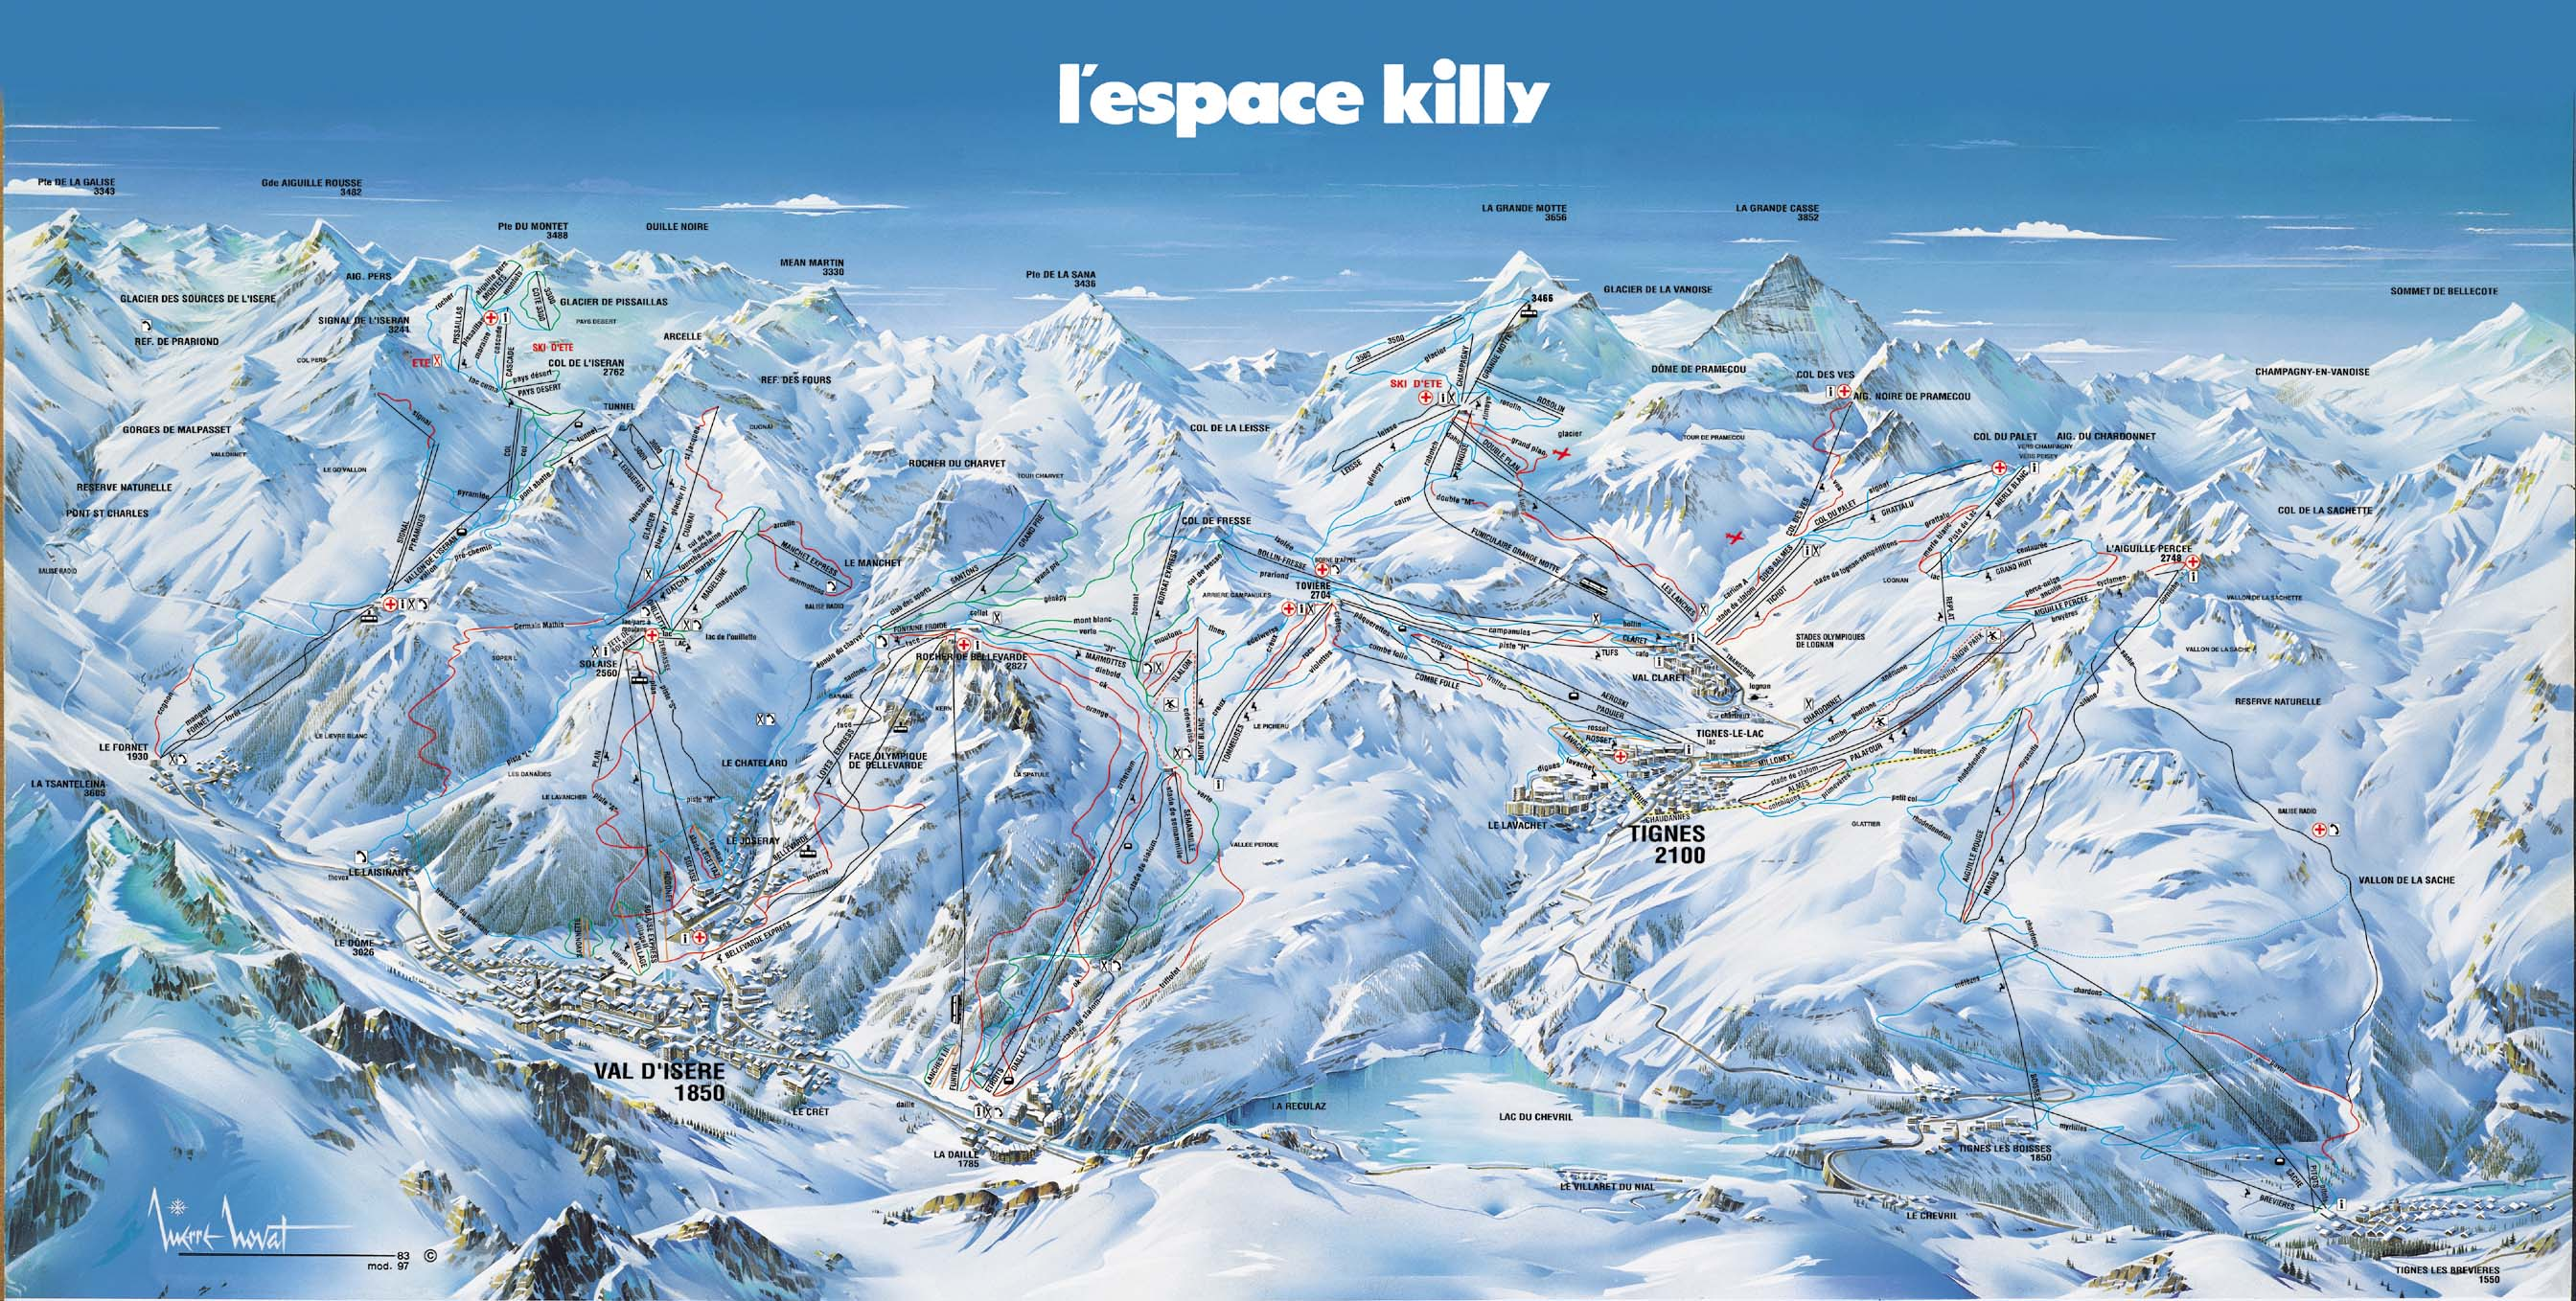
\includegraphics[width=1.0\linewidth]{novat/PN_killy.jpg}
 \caption{\label{killy} Espace Killy (Val D'Isere, Tignes) par Pierre Novat}
\end{figure*}

 Un panorama est une représentation visuelle grand angle d'un espace physique. Cette image, prise d'un point de vue particulier, généralement surélevé, permet d'avoir une vue d'ensemble sur une région donnée. C'est une œuvre artistique, où l'artiste, en photo, en peinture ou en dessin peut choisir de mettre en avant certains éléments au détriment d'autres. Les cartes panoramiques sont des panoramas particuliers ayant pour but de servir de carte à un utilisateur non-expert. En effet la vue dégagée d'un panorama permet de se repérer et de s’orienter. De plus les artistes qui créent ces panoramas sont aussi des experts en cartographie. Seulement, la création de panorama est un processus long et compliqué et le savoir-faire commence tout doucement à se perdre avec l'arrivée des outils informatiques qui permettent la création rapide de cartes. Cependant ces cartes ne sont pas de la même qualité que les cartes panoramiques faites par des artistes qui vont toujours chercher à faire aimer la région qu'ils représentent en prenant en considération des éléments autres que géographiques. Ainsi vient la question de l'automatisation des panoramas en essayant de produire un résultat proche de ce que pourrait produire un artiste. C'est un objet d’étude intéressant pour une recherche sur la question de la stylisation de modèles 3D car les panoramas posent de façon cruciale la question de comment et quoi représenter pour une application très spécifique : permettre une lecture utile et esthétique du paysage. C’est aussi un cas d’étude permettant d’explorer la marge de manœuvre à laisser au designer dans le processus de création : un  compromis à faire entre contrôle et automatisation.
 
Dans notre coté, nous nous intéressons au rendu de panorama de montagnes, plus particulièrement dans le style de l'atelier Pierre Novat (Fig. \ref{killy}). Pour comprendre le processus de création de ces panoramas, nous avons travaillé avec l'aide d'Arthur Novat. Cette collaboration nous a permis d'expliciter un ensemble de règles qu'il utilise pour la création de ses panoramas pour pouvoir ensuite les traduire en algorithme pour produire un rendu dans le style Novat. Nous nous sommes plus spécifiquement intéressés au calcul d'un ombrage qui donne à voir le relief d'un terrain montagneux et pourra servir de base au dessin d'un panorama. 

Dans ce rapport, nous présentons dans un premier temps notre étude sur le style des panoramas de Pierre Novat  pour comprendre comment chaque élément est construit, notamment les ombres et la lumière. Dans un second temps nous étudions la manière qu'ont les cartographes de dessiner les ombres et les précédents travaux en informatique graphique sur les ombres, en particulier \textit{exagerated shading} \cite{rusinkiewicz2006exaggerated} qui propose un ombrage orienté vers la cartographie. Ensuite nous présentons notre solution pour calculer un ombrage expressif construit à l'aide des précédentes études et des règles que nous avons produites. Enfin nous montrons notre méthode de validation et les travaux futurs. 


\begin{figure*}[h!]
\centering
 \begin{subfigure}[t]{0.49\linewidth}
   \centering
   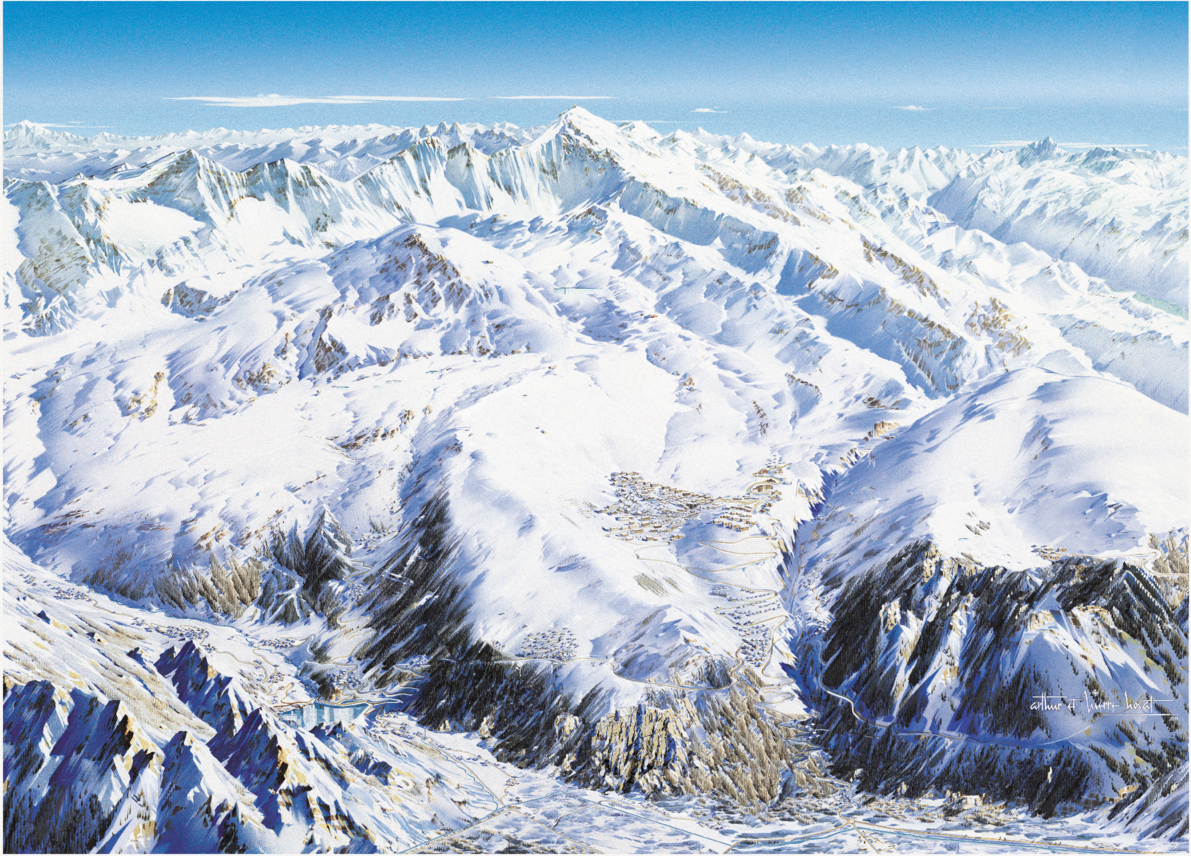
\includegraphics[width=1.0\linewidth]{novat/AlpeHuez.png}
   \caption{Sans les pistes}
 \end{subfigure}
 \begin{subfigure}[t]{0.49\linewidth}
   \centering
   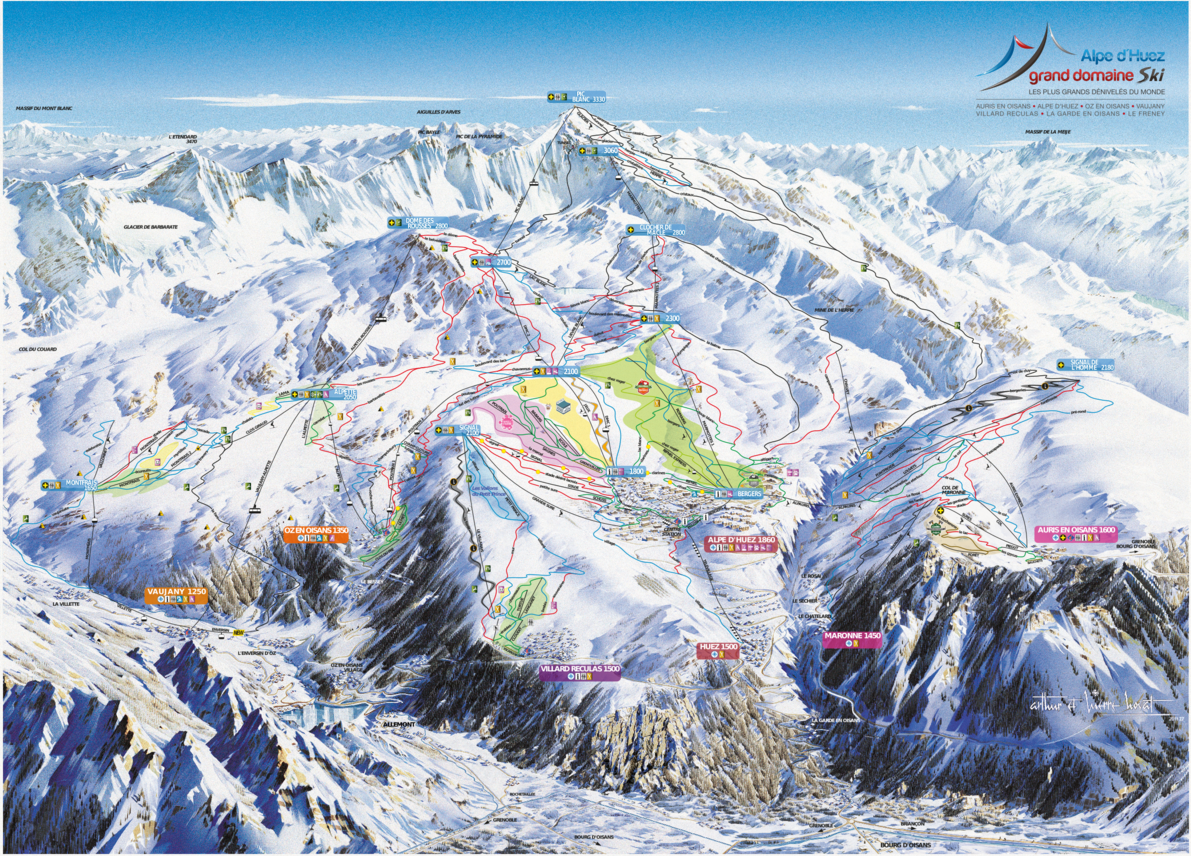
\includegraphics[width=1.0\linewidth]{novat/AlpeHuez_pistes.png}
   \caption{Avec les pistes}
 \end{subfigure}
 \caption{L'Alpes d'Huez par Arthur et Pierre Novat}
\end{figure*}

\chapter{\label{chap:Novat} Le Style Novat}


\section{Contexte}


Parmi les panoramistes reconnus, Pierre Novat est l'artiste qui a dessiné et peint la plupart des panoramas des domaines skiables de France. Il travaillait avec des commanditaires locaux pour produire des panoramas de montagne servant de support aux plans des pistes du domaine skiable. Son travail était avant tout destiné aux habitants locaux et aux skieurs et était régi par des contraintes de politiques locales.

Aujourd'hui décédé, c'est son fils, Arthur Novat, qui a repris l'atelier et le travail de son père.  Pour empêcher que cette disparition entraîne une perte du savoir-faire de l'atelier, Arthur Novat essaye de transmettre son savoir et ses techniques à des chercheurs pour que celle-ci perdurent. 

Ainsi pour préserver la mémoire et la compréhension du travail de Pierre Novat, en 2015 débute le projet "MÉmoire, COnnaissance et MOdélisation de la Montagne : innovations et transfert d'outils de conception de plans panoramiques" (MECOMO) \footnote{MECOMO : \url{http://www.labexitem.fr/projet/memoire-connaissance-et-modelisation-de-la-montagne-innovations-et-transfert-doutils-de}}. C'est une collaboration entre géographes cogniticiens (INRIA), historiens (LARHRA) et informaticiens (LIG), autour de la conception de plans de pistes de ski par l'atelier Novat depuis la fin des années 1960. L’objectif global vise à reconstituer le fonctionnement de cette représentation dans le temps et donc dans l’évolution d’un système (les stations de ski), de manière à mieux comprendre le processus d’adéquation entre besoins, usages et représentation de l’espace au fil des années.
Cela s'articule autour de 3 axes : 
\begin{enumerate}
\item Historique: l’évolution des domaines skiables dans les Alpes et de ce qui les entoure. 
\item Cognition: la création et la lecture des panoramas de l'atelier Novat.
\item Informatique: l'automatisation de la création de panoramas.
\end{enumerate}

Ce projet a pris fin en 2017. Entre temps, plusieurs études ont été publiées notamment sur la création mental puis artistique d'un panorama fait par l'atelier Novat \cite{balzarini2015study} et sur l'analyse de la lecture des panoramas style Novat par les usagers \cite{balzarini2016effectiveness}. De plus un logiciel prototype a été créé au LIG pour permettre à un utilisateur de déformer des montagnes.  
Cependant, il reste encore beaucoup de recherche à faire pour pouvoir produire automatiquement des panoramas "à la Novat". 

En nous appuyant sur les études du projet MECOMO et en travaillant avec Arthur Novat, notre objectif est ainsi d'expliciter des règles de dessin et de les mettre en œuvre dans une application informatique. 
La production d'un logiciel prototype pour la création de panoramas permettra d'aider à la formalisation des règles et de les valider.

\section{Les panoramas de montagnes en informatique graphique}

Il y a deux travaux scientifiques qui ont été faits sur le rendu complet de panoramas de montagnes en informatique graphique. 

Le premier a été fait par Bratkova et al. en 2009 \cite{bratkova2009artistic}. Dans leur papier ils analysent les œuvres de Berann et James Niehus, deux artistes spécialisés dans les panoramas, et proposent un ensemble de principes pour le rendu de panoramas. Leur algorithme inclut des méthodes pour la déformation de terrain, la génération d'ombrage et de texture. Leurs résultats correspondent aux styles de Berann et James Niehus, toutefois leur méthode ne permet pas un rendu temps réel. 

Le second, fait par Brown et al. en 2017 \cite{brown2017real}, s'appuie sur les résultats du premier. Il présente une méthode pour un panorama interactif temps réel d'une région donnée. Comme pour le premier, leur algorithme inclut des méthodes sur la déformation de terrain, le rendu des couleurs (ombrage), le rendu des arbres, de l'eau et de l'atmosphère. Cependant, ces deux études n'explorent qu'en surface les différents éléments qui composent un panorama et produisent des résultats ressemblant mais loin d'être parfaits et qui comportent beaucoup de défauts. 

Nous allons suivre la même méthodologie que ces travaux : étudier le style de Pierre Novat pour en produire des règles de dessin et ensuite les appliquer dans un rendu 3D.



\section{Étude du style de Pierre Novat}

Pour cette étude, nous nous basons sur le livre : le plan des pistes, les domaines skiables de France dessinés par Pierre Novat \cite{novat2013plans} qui contient ses panoramas accompagnés de notes écrites par Frédérique Novat, Arthur Novat et Laurent Belluard, ainsi que sur les différentes interviews que nous avons pu faire avec Arthur Novat. Cependant cela reste des panoramas fait à la main et donc même si les règles citées ci-dessous sont généralement respectées, il existe toujours des contre-exemples.



\subsection{Qu'est-ce que dessiner un panorama du point de vue d'Arthur Novat ?}
Un panorama répond à la demande d’un commanditaire qui veut donner à voir une montagne de façon à la mettre en valeur. Cette demande porte en elle une part de fausseté car la représentation recherchée ne correspondra jamais à un point de vue réel. C’est une représentation d’un territoire imaginaire dans le but de le décrire au mieux et de le faire aimer. 
Le commanditaire est généralement un acteur important de la région : station de ski, collectivité locale, comité d'organisation des Jeux olympiques d'hiver, etc.

Le panorama des pistes de ski doit donc suivre certaines contraintes pour satisfaire le commanditaire mais aussi le skieur. Tout d'abord, les conditions météo et de luminosité doivent être optimales: avoir un ciel dégagé et un soleil matinal plutôt rasant révélant l'ensemble du relief. Ensuite, le panorama doit être équilibré géographiquement, c'est-à-dire que les étages alpins doivent être respectés : un point qui est en plus haute altitude qu'un autre, doit l'être sur le panorama. Même principe pour les dénivelés: plus une pente est inclinée, plus elle doit l'être sur le panorama. Enfin, au-delà des aspects purement géographiques les panoramas doivent aussi obéir à des contraintes sociales et politiques, c'est-à-dire qu'il faut respecter la concurrence entre les commendataires et la vision de la population locale. En effet, les villages présents sur le panorama veulent avoir une taille proportionnelle à leur investissement dans la station. Mais il faut aussi que la population locale puissent reconnaître sa région dans le panorama en ayant un point de vue reconnaissable ou des éléments marquants du paysage mis en avant. Par exemple Chamrousse est une station de ski visible depuis Grenoble et utilisée principalement par ses habitants donc le panorama a comme point de vue celui de Grenoble. 
D'un autre coté, les lieux importants doivent être mis en valeur et au contraire les lieux moins accessibles doivent être amenuisés. Enfin, les pistes doivent avoir une bonne représentation: elles doivent toujours descendre, les types de pistes (verte, bleue, rouge ou noire) doivent être vues de la même façon (même si en réalité les pistes vertes sont plus courtes que les noires), et le lecteur doit pouvoir différencier les pistes noires des pistes vertes uniquement grâce à leur forme (sinueuse pour les vertes, droite pour les noires).


\subsection{Fabrication en pratique - Les différentes étapes}

\begin{figure*}[h!]
\centering
 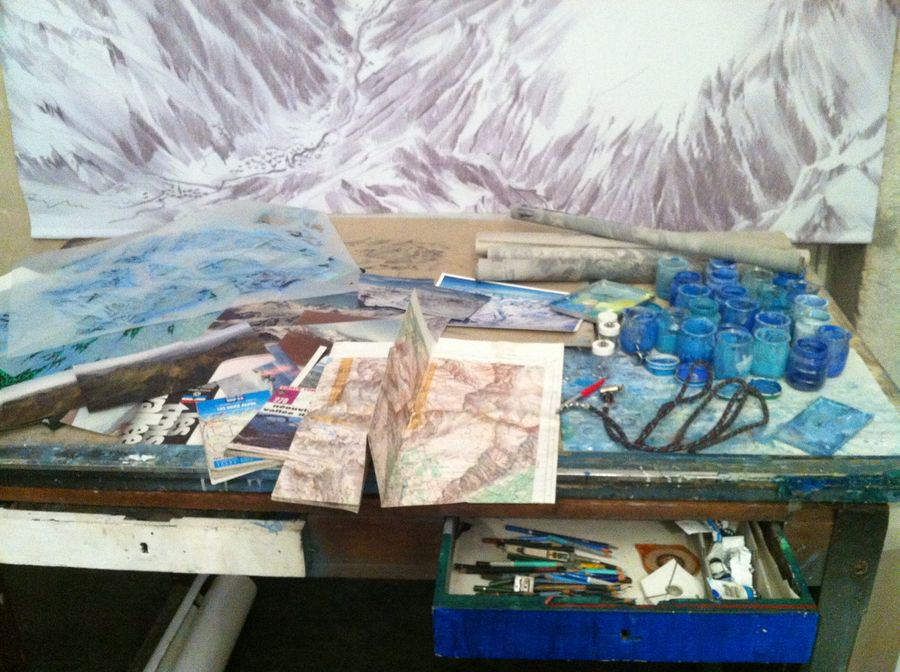
\includegraphics[width=0.5\linewidth]{novat/PN_Modelisation.jpg}
 \caption{\label{fig:Model} Pêle-mêle de photos et de cartes}
\end{figure*}


Maintenant que nous avons vu les règles générales des panoramas style "Novat", nous nous penchons sur la fabrication concrète d'un panorama. Pour faire des panoramas Pierre Novat utilisait, en fonction des territoires et de son inspiration, de la gouache, un aérographe, des feutres et des crayons de couleur; le tout appliqué sur une couche d'acrylique Gesso. Il y avait aussi un cheminement précis pour la création d'un panorama mis en place par l'atelier Novat : 
\begin{enumerate}
%\baselineskip=10pt
\item Le point de départ est une carte d'état major, de l'Institut national de l'information géographique et forestière (IGN) TOP25 ou autre. Elle sert à comprendre le terrain (Arthur Novat interprète les courbes de niveau comme un volume) et à choisir le point de vue.
\item Une collecte d'information s'ensuit : étude de la nature du terrain, photos (au sol, en avion, satellite) et visite sur place. Le but est de comprendre la physionomie du paysage. 
\item Prise en compte de la demande du commanditaire en dépliant le paysage. Construction d'un pêle-mêle de photos et de cartes. (Fig. \ref{fig:Model})
\item Création d'un crayonné à partir du pêle-mêle (calque et crayon ou photoshop). Un crayonné est un dessin en niveau de gris qui correspond principalement à l'ombrage mais il contient aussi toutes les éléments nécessaires au panorama (Fig. \ref{fig:crayonne}).
\item Validation par le commanditaire.
\item Mise en couleur :
\begin{enumerate}
\item Décalquage du crayonné au crayon de couleur (colorier au crayon de couleur sur un calque, le retourner sur le support et tracer l'esquisse).
\item Ajout de soutiens : crayon de couleur pour soutenir les arêtes ou les zones saillantes. 
\item Application d'une couche d'aérographe à la gouache avec utilisation de rhodoïds pour masquer.
\end{enumerate}
\item Dessin des détails : (Fig. \ref{fig:courchevel})
\begin{itemize}
\baselineskip=10pt
\item Sapins au crayon de couleur;
\item Rochers en peinture et crayons;
\item Maisons en peinture et crayons;
\item Rehausse du blanc en peinture;
\item Gratter sur le gesso pour retrouver le blanc. 
\end{itemize}
\end{enumerate}



\begin{figure*}[h!]
\centering
 \begin{subfigure}[t]{0.47\textwidth}
 \centering
 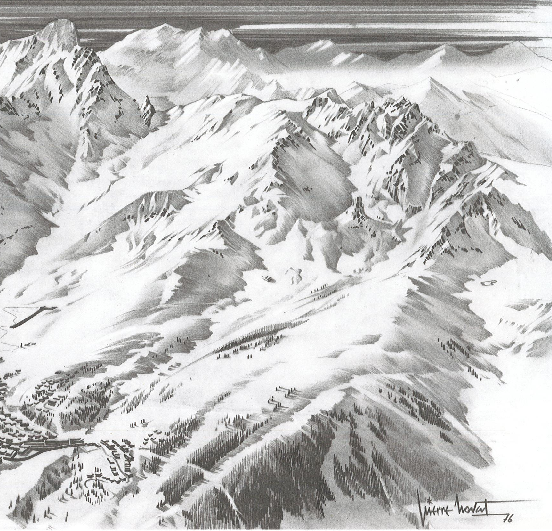
\includegraphics[width=1.0\linewidth]{novat/crayonn_.png}
 \caption{\label{fig:crayonne} Version crayonnée}
 \end{subfigure}%
 ~
 \hspace{.05\textwidth}
 \begin{subfigure}[t]{0.47\textwidth}
 \centering
 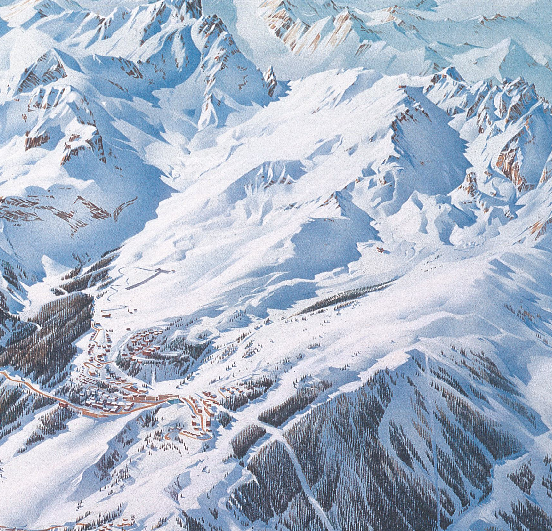
\includegraphics[width=1.0\linewidth]{novat/courchevel.png}
 \caption{\label{fig:courchevel} Version colorisée}
 \end{subfigure}
 \caption{Le panorama de Courchevel par Pierre Novat}
\end{figure*}



\subsection{Éléments visuels spécifiques du style Novat}
Intéressons-nous maintenant plus en détail à ces panoramas de style "Novat". Ils contiennent plusieurs éléments visuels qui n'ont pas la même importance. En effet si certains sont purement décoratifs, d'autres sont essentiels à la lecture et la compréhension du panorama. Nous décrivons ci-dessous les éléments visuels principaux par ordre d'importance.



\begin{figure*}[!h]
\centering
 \begin{subfigure}[t]{0.47\textwidth}
 \centering
 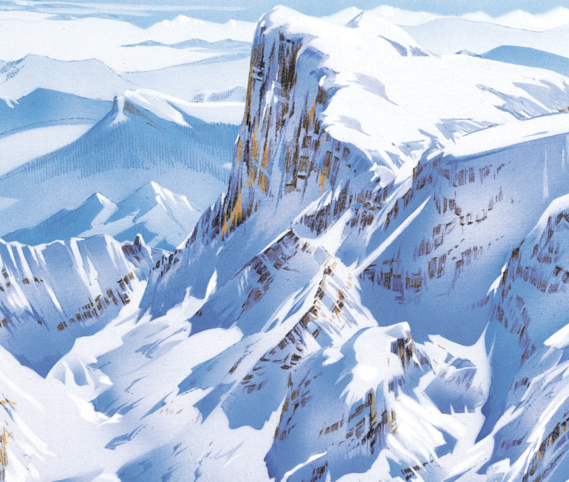
\includegraphics[width=1.0\linewidth]{novat/PN_zoom_ombre.png}
 \caption{\label{fig:zoom_ombre} Des ombres incohérentes mais lisible}
 \end{subfigure}%
 ~
 \hspace{.05\textwidth}
 \begin{subfigure}[t]{0.47\textwidth}
 \centering
 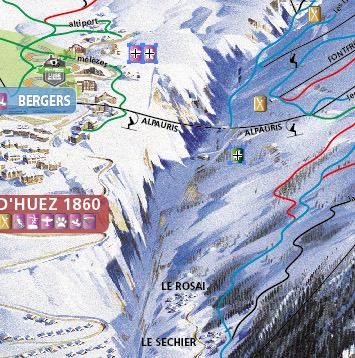
\includegraphics[width=1.0\linewidth]{novat/ombres_zoom.jpg}
 \caption{\label{fig:OmbrePortées} Ombres portées marquées sur le bord mais plus légères sur le flan de la montagne}
 \end{subfigure}
 \caption{\label{fig:ExOmbres} Exemples d'ombrage. %\ro{dans les 2 exemples, ce serait bien de mettre des flèches pour savoir exactement ou regarder (par ex: à quel endroit l'ombrage est différent d'un autre?)}
 }
\end{figure*}


\paragraph*{La lumière et les ombres :} 
Les variations d'intensité produites par l'illumination sont l'indice visuel principal pour comprendre la forme de la montagne. Elles peuvent ses séparer en deux composantes : ombrage et ombres portées. Ce sont toutes deux un signe d'une absence de lumière mais du à des causes différentes. Elles répondent à deux questions différentes : 
\begin{itemize}
\baselineskip=10pt
\item L'ombrage détermine si la surface est face à la lumière ou non. 
\item Les ombres portées déterminent si un autre élément cache la lumière. 
\end{itemize}
De plus le jeu des ombres amène des contrastes forts et tranchés qui donnent toute la nervosité du style de Novat. Seulement cette lumière est très irréaliste. Bien qu'il y ait une direction générale de la lumière (qui vient d'en haut, à droite ou à gauche), si nous regardons plus en détail, nous constatons que celle-ci n'est pas constante et peut être parfois totalement incohérente. Ainsi elle va plus être dirigée par la pente et les éléments que l'artiste veut montrer que par le respect de la réalité (Fig. \ref{fig:zoom_ombre}).
Enfin les ombres portées ne sont pas en conflit avec l'ombrage. En effet, les ombres portées sont rajoutées comme une couche supplémentaire plus légère que l'ombrage pour souligner le relief global sans pour autant gêner l'ombrage.  Aussi il est important de noter que tout a une ombre, que ce soient les montagnes, les petites bosses, les arbres, les maisons ou les routes. Ces ombres vont être orientées selon la forme de l’élément et la pente sur laquelle il repose.



D'autre part, les ombres ne sont pas d'une couleur uniforme (Fig. \ref{fig:OmbrePortées}) . Cela vient de deux facteurs. Le premier est que la montagne peut réfléchir la lumière et donc la montagne qui lui fait face aura une tache lumineuse pour indiquer cette inter-réflexion. Le second vient de la méthode de dessin. Pour dessiner ces ombres Arthur Novat va mettre un coup de crayon ou de couleur le long de l'ombre (généralement en bas), puis il va aplatir et étirer ce trait en le faisant remonter le long de la pente. Enfin les ombres sont très anguleuses. 
Tout ce travail a pour but de rendre très claire la lecture de la montagne et de la comprendre.









\paragraph*{La neige :} C'est un élément assez important car elle permet de connaître la nature du terrain. Il y a 3 types de terrain qui se dégagent : les glaciers qui sont verts et assez lumineux, la neige sur pente molle qui est très claire et réfléchissante et enfin la neige sur pente dure qui est plus sombre et mate. De plus la neige a un dégradé de couleur entre la haute altitude et la basse altitude. En haute altitude, la neige est proche du vert à cause des glaciers. En basse altitude par contre la neige sera plus bleue du fait de l’atmosphère.  


\paragraph*{Les arbres :} Leur importance vient de leur organisation. Le but de cette organisation est d'améliorer la perception de la forme de la montagne en plus des ombres. Pour ce faire, ils sont alignés verticalement et dans le sens de la pente. De plus il peut y avoir un trait sombre sur le bas des forêts pour marquer les ruptures de pente. 
Les arbres sont de couleur verte, allant du vert très foncé presque noir à l'ombre au marron-vert et quelque fois vert très clair en lumière. Il existe aussi quelques sapins blancs. Enfin ils sont toujours dessinés de manière verticale. Au $1^{er}$ plan, ils ont une forme légèrement triangulaire, au fond ils sont ovales, très fins et pointus au bout.  




\begin{figure*}[h!]
\centering
 \begin{subfigure}[t]{0.47\textwidth}
 \centering
 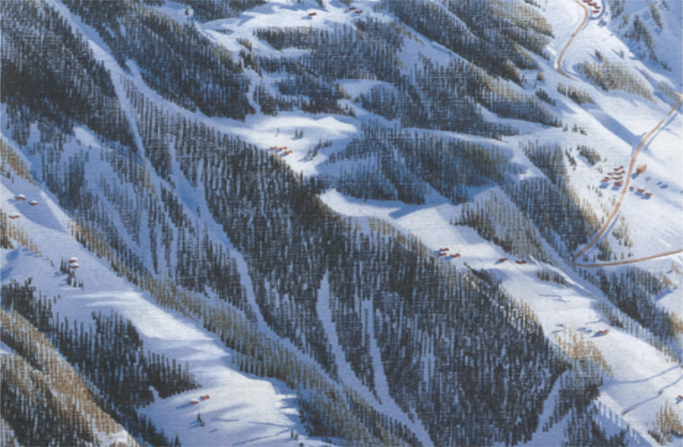
\includegraphics[width=1.0\linewidth]{novat/arbres_zoom.png}
 \caption{\label{fig:foret} Une foret sur un flan de montagne}
 \end{subfigure}%
 ~
 \hspace{.05\textwidth}
 \begin{subfigure}[t]{0.47\textwidth}
 \centering
 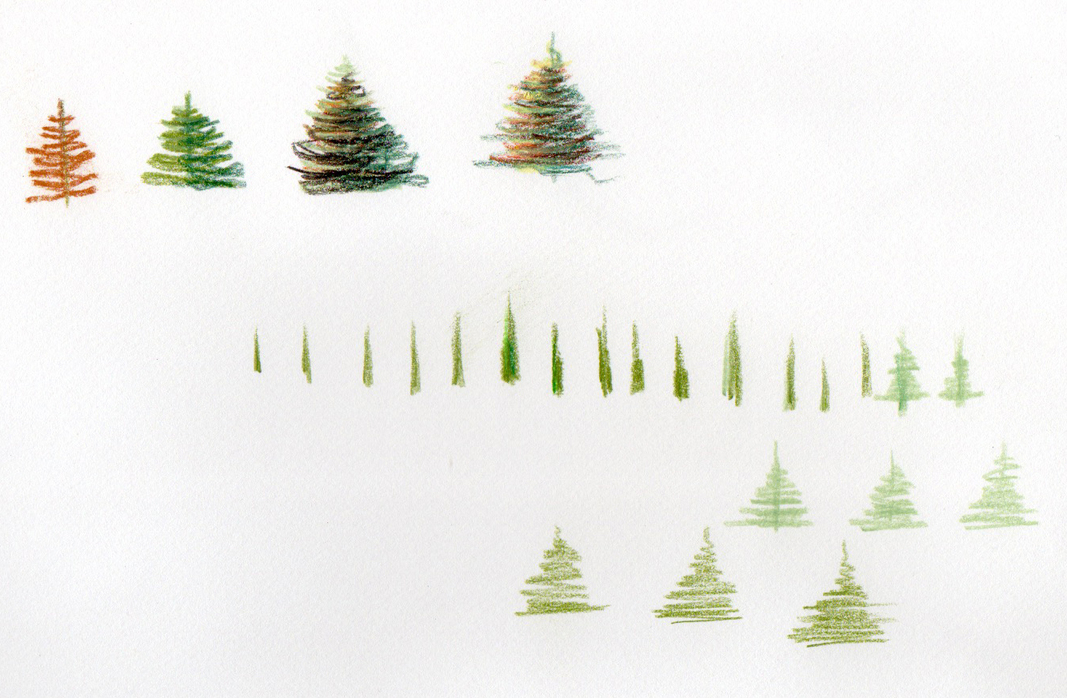
\includegraphics[width=1.0\linewidth]{novat/novat_arbre.jpeg}
 \caption{\label{fig:sapinseuls} Sapins dessinés par Arthur Novat}
 \end{subfigure}
 \caption{\label{fig:ExArbres} Exemples d'arbres}
\end{figure*}


\paragraph*{Les roches :} Elles sont moins importantes que les autres éléments cités plus haut mais elles ont quand même deux utilités. Elles sont soit informatives : elle servent à indiquer les barres rocheuse ou les pentes très raides où la neige ne peut pas tenir, donc des zones dangereuses; soit décoratives et servent de point de repère pour des zones rocheuses très identifiables de la région. Ainsi les roches sont organisées le plus souvent en lignes horizontales qui peuvent faire penser à des strates. Mais ces lignes ne sont pas continues, il y a toujours de fines bandes de neige qui passent entre les rochers et les délimitent. Enfin, elles se situent la plupart du temps juste en dessous des sommets des montagnes (Fig. \ref{fig:falaise}).

La couleur des rochers est unie. Elle va du gris clair, marron clair en lumière au marron foncé, noir à l'ombre. Leur forme est rectangulaire mais suit la forme de la montagne. La taille d'une roche varie selon la forme de la montagne (Fig.\ref{fig:rochersseul}).



\begin{figure*}[h!]
\centering
 \begin{subfigure}[t]{0.47\textwidth}
 \centering
 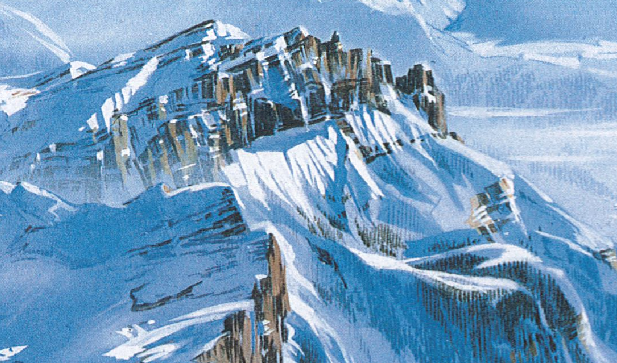
\includegraphics[width=1.0\linewidth]{novat/rochers_zoom.png}
 \caption{\label{fig:falaise} Une falaise}
 \end{subfigure}%
 ~
 \hspace{.05\textwidth}
 \begin{subfigure}[t]{0.47\textwidth}
 \centering
 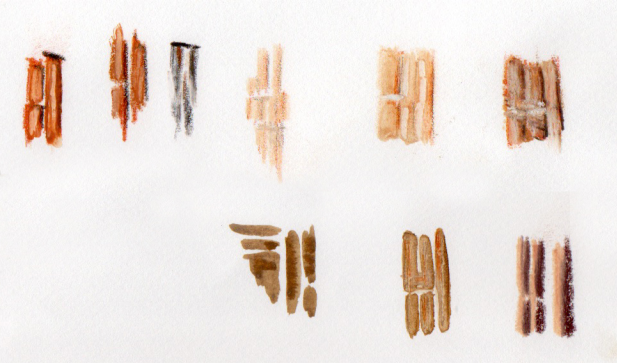
\includegraphics[width=1.0\linewidth]{novat/novat_roches.png}
 \caption{\label{fig:rochersseul} Roches faites par Arthur Novat}
 \end{subfigure}
 \caption{\label{fig:ExRoche} Exemples de roches}
\end{figure*}

\paragraph*{Les Maisons :} Purement décoratives, les maisons représentent les villes et villages de la région. Marron avec un toit blanc, leurs formes sont minimalistes mais correspondent à la réalité. Leur utilité est de servir de point de repère (Fig. \ref{fig:ExMaison}).


\begin{figure*}[h!]
\centering
 \begin{subfigure}[t]{0.47\textwidth}
 \centering
 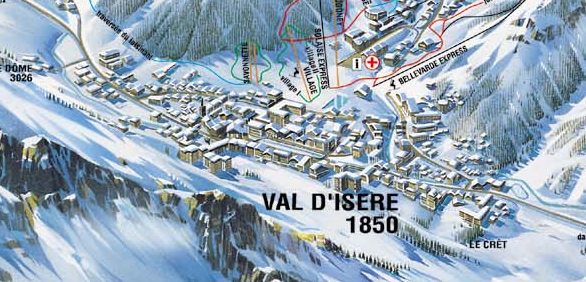
\includegraphics[width=1.0\linewidth]{novat/PN_maison.png}
 \caption{\label{fig:village} Le village de Val D’Isère}
 \end{subfigure}%
 ~
 \hspace{.05\textwidth}
 \begin{subfigure}[t]{0.47\textwidth}
 \centering
 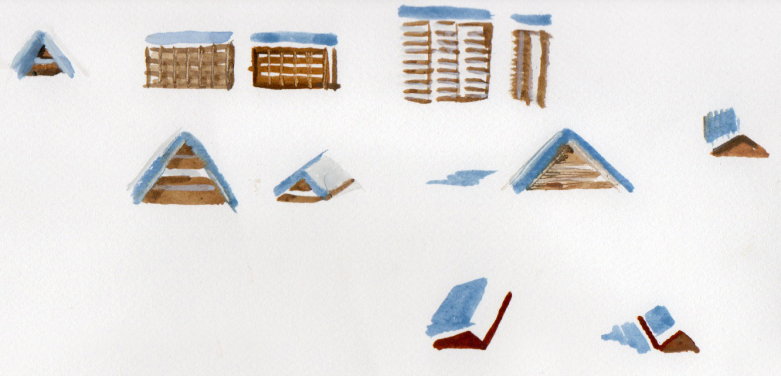
\includegraphics[width=1.0\linewidth]{novat/novat_maison.png}
 \caption{\label{fig:maisonsseul} Maisons faites par Arthur Novat}
 \end{subfigure}
 \caption{\label{fig:ExMaison} Exemples de maisons}
\end{figure*}

\paragraph*{Les routes :} Dessinées d'un trait continu, elles suivent fidèlement les routes existantes. Elles forment un creux dans la neige là ou elles passent. 

\paragraph*{L’arrière plan :}
Il est constitué uniquement de montagnes dessinées beaucoup plus simplement et avec bien moins de détails. Néanmoins, ces montagnes reste identifiables et reconnaissables pour quelqu'un qui connaît la région (Fig. \ref{fig:ciel}). 

\paragraph*{Le ciel :} Il est dégradé de bleu, avec quelques nuages. D'un bleu assez clair en bas, il fini très sombre en haut du panorama.   

\begin{figure*}[!t]
\centering
 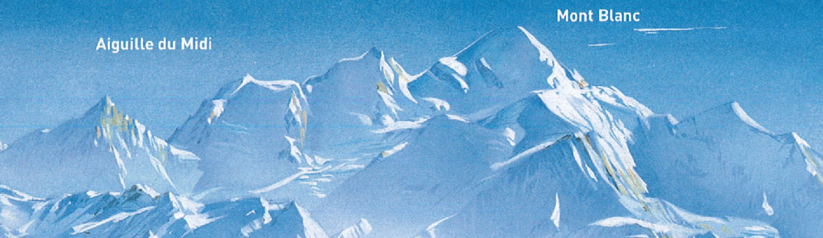
\includegraphics[width=1.0\linewidth]{novat/ciel_zoom.png}
 \caption{\label{fig:ciel}L'arriere plan du panorama du Grand Massif avec l'aiguille du Midi et le Mont Blanc qui sont reconnaissable}
\end{figure*}

\chapter{État de l'art sur l'ombrage}
\section{Problématique}


Au vu de l'étude du style, nous voyons que chaque élément visuel suit des règles spécifiques. Donc pour automatiser fidèlement le style il faut automatiser spécifiquement chaque élément. Nous avons vu que l'élément le plus important était l'ombrage, c'est donc sur cet élément visuel que nous allons travailler. 

Ainsi notre contribution à ce travail à été de faire un rendu des ombres le plus fidèle aux panoramas de l'atelier Novat. Notre problématique étant de faire un ombrage de manière a voir la maximum d’éléments sur la surface d'une montagne. Pour ce faire, en plus de nous baser sur le style de l'atelier Novat, nous nous sommes appuyés sur les techniques des cartographes, ainsi que le traitement des ombres non réaliste en informatique graphique. 

\section{L'ombrage vu par les cartographes}

\begin{figure}[!h]
	\centering
 	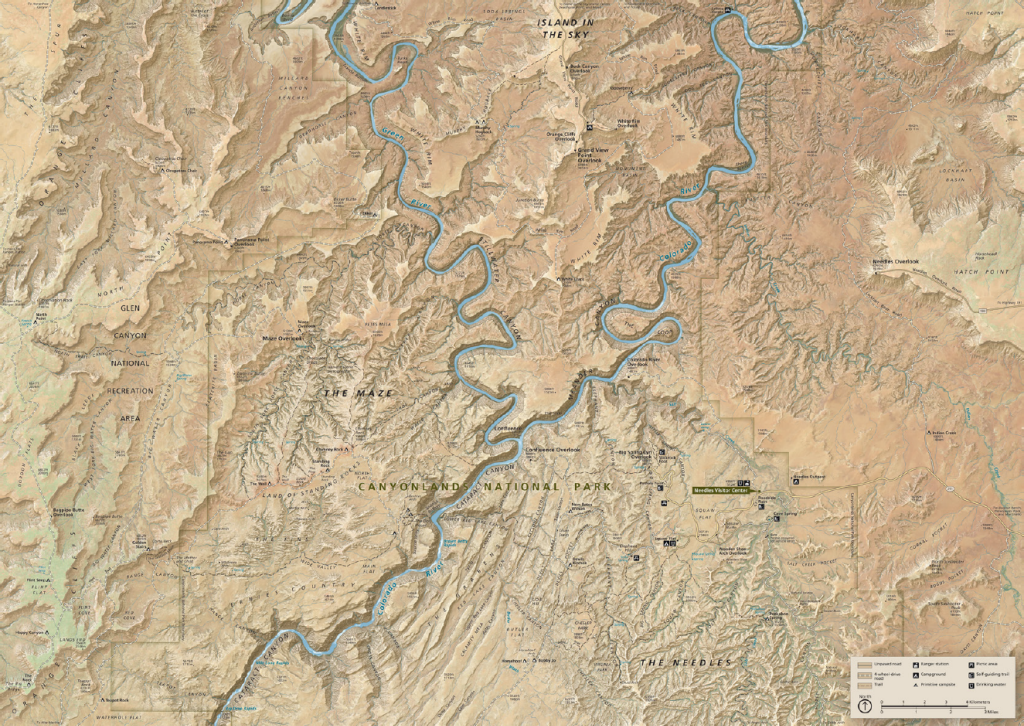
\includegraphics[width=0.7\linewidth]{Etat_de_l_art/carte_Paterson.png}
 	\caption{\textit{The Heart of Canyonlands National Park} par Tom Paterson}
\end{figure}
Pour cette étude, nous nous sommes basés sur les conseils et remarques du cartographe Tom Paterson\footnote{Le site de Tom Paterson où sont référencés tous ses conseils sur l'ombrage de relief : \url{http://www.reliefshading.com/}} \cite{patterson2000view}\cite{patterson2005looking}. Il est important de noter que tous les cartographes n'ont pas la même approche ni le même point de vue sur la façon de faire des cartes. Cependant Tom Paterson reste une référence fiable dans ce domaine.

Que ce soient des cartes vues de dessus ou d'un point vue panoramique, le dessin des ombres est une partie très importante en cartographie. La règle la plus importante est que l'ombrage des reliefs doit décrire la forme du terrain d'une manière descriptive et facilement mesurable. Ainsi la question est : quelles ombres l'artiste doit représenter ? Il y a 2 types d'ombres : l'ombrage et les ombres portées. Si la première ne va qu'assombrir certaines zones, l'autre va projeter la forme d'un élément sur un autre.

Dans la nature, ces deux types sont confondus mais, selon Parterson, uniquement l'ombrage est utilisé en cartographie car les ombres portées peuvent rendre difficile à lire les cartes et peuvent mener à de mauvaise interprétation du terrain. Malgré cela Pierre Novat utilise les ombres portées mais elle sont moins importantes et plus claires que l'ombrage afin de ne pas gêner la lecture. 

Un élément important est de bien définir la direction de la lumière. Même si l'orientation de la lumière par rapport au Nord, que nous appelons azimut, est propre à chaque cartographe, la hauteur (ou élévation), elle, est constante. Elle varie, d'une carte à l'autre, entre $20\degres$ et $50\degres$ mais elle est plus généralement aux alentours de $45\degres$. Une technique essentielle est de réajuster l'azimut de cette lumière localement pour permettre de mieux voir certaines variations de terrain (cf Fig. \ref{fig:corretionLumière}). 


\begin{figure}[!t]
	\centering
 	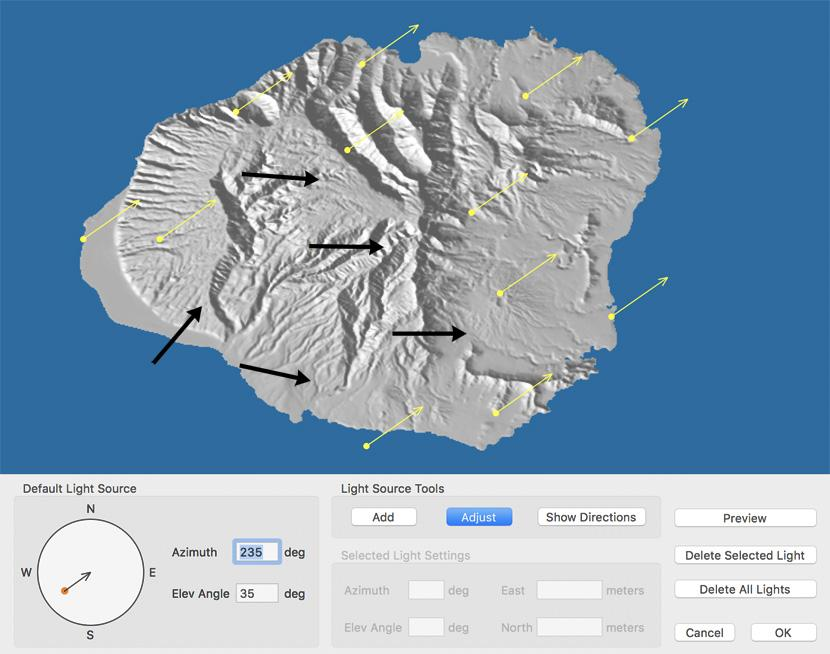
\includegraphics[width=0.7\linewidth]{Etat_de_l_art/multiple_light.jpeg}
 	\caption{\label{fig:corretionLumière}Correction locale de la lumière. Les flèches jaunes représentent la lumière globale, les flèches noires les corrections locales faites par l'artiste.}
\end{figure}

Enfin il existe une autre technique pour améliorer la lecture d'une carte. Le principe est de rendre deux cartes d'ombres. L'une avec un fort contraste, l'autre avec un contraste plus faible pour avoir de meilleurs détails. Ensuite il suffit de les fusionner ensembles avec une interpolation linaire. Cette technique permet d'obtenir les meilleure caractéristiques de chacune. C'est sur ces deux derniers principes que nous baserons notre calcul d'ombrage.




\section{Exagération de la forme en informatique graphique }


La représentation de la forme est une question importante en informatique graphique. Pour pouvoir mieux la percevoir, beaucoup de travaux vont proposer d’exagérer cette forme. Une approche courante est d'utiliser des techniques de rendu à base de lignes pour modifier cette forme. Le principe est d'utiliser la géométrie de l'objet pour ensuite en détecter la forme  en utilisant par exemple la courbure \cite{ohtake2004ridge} et dessiner uniquement les contours de cet objet \cite{zhang2009laplacian}. Seulement, ces techniques ne permettent pas de voir toute les variations d'une forme mais uniquement des zones très localisées comme les crêtes et les vallées. Ainsi utiliser l'ombrage permet de palier à ce problème. 

\paragraph*{Perception de la forme grâce à l'ombrage}
L'ombrage est un élément essentiel en informatique graphique, il permet de percevoir la forme des objets d'une scène et de distinguer leurs détails. Ainsi cette perception peut être manipulée, comme le montrent Vergne et al. dans une étude publiée en 2016 \cite{vergne2016flow} dans laquelle ils modifient l'ombrage des objets pour en modifier la perception. Des études perceptuelles comme celles de Caniard et al. \cite{caniard2007distortion} montrent en effet que l'utilisation d'une unique source lumineuse sur un objet va modifier la perception de cette objet selon la position de souce et donc qu'une unique source de peut pas permettre la perception de toute la forme de l'objet. De plus, dans une étude de 2010, Lopez et al.~\cite{lopez2010measuring} font l'expérience suivante : dans une scène où 0, 1 ou 2 objets sur 6 objets, sont éclairés avec un angle de lumière différent, ils demandent à des sujets de les identifier. Le résultat montre que le cerveau humain n'arrive pas à percevoir cette différence d'angle. Ainsi l'ensemble de ces études montrent que 1: la direction de la lumière est primordiale pour bien percevoir la forme d'un objet et 2: notre perception visuelle a bien du mal à estimer la direction de la lumière. Nous pouvons donc modifier celle ci pour mettre en valeur le relief, tout en conservant une cohérence globale.

\paragraph*{Modification de l'ombrage}
Pour augmenter la perception de la forme grâce à l'ombrage, il existe plusieurs approches. Une technique très utilisée est celle de l’occlusion ambiante proposée par Pharr et Green \cite{pharr2004ambient}. En se basant sur une technique introduite par Miller et al. \cite{miller1994efficient} qui permet de détecter les cavités sur une surface 3D, ils les utilisent pour modifier localement l'ombrage et ainsi faire mieux ressortir ces cavités. Cette méthode a néanmoins tendance à faire ressortir uniquement les cavités profondes tout en lissant les moins profondes. Une autre approche proposée par Ritshel et al. \cite{ritschel20083d} est d'utiliser l'illusion de Cornsweet pour créer un masque qu'il applique sur un ombrage classique. Le problème est que cela va augmenter les contrastes si un flan de montagne est vraiment dans l'ombre et donc cela ne permet pas de "déboucher" les ombres. 

Une autre solution publiée par Zhang et al. \cite{zhang2010perceptually} est d'uniquement modifier la normale à l'aide de la courbure de l'objet de manière à optimiser la perception des aspérités de l'objet.
Un travail similaire publié par Vergne et al. \cite{vergne2008apparent} propose un ombrage uniquement basé sur la courbure d'un objet. À cette courbure ils assignent une carte de relief, c'est-à-dire que pour chaque valeur de courbure ils associent une valeur d'ombre comprise entre $0$ et $1$. Le problème de ces 2 approches c'est qu'en plus de ne pas avoir de lumière globale, elles utilisent la courbure qui en cartographie n'est pas une information pertinente pour calculer un ombrage qui met en valeur les montagnes. Dans notre approche nous utiliserons plutôt la pente.

\paragraph*{Exagerated Shading}
Une technique introduite par Rusinkiewicz et al. \cite{rusinkiewicz2006exaggerated} et plus proche de notre solution est d’exagérer l'ombrage afin d'avoir une meilleure perception des aspérités d'une surface. Le principe est de faire un ombrage sur plusieurs échelles, chaque échelle ayant un niveau de flou différent. Pour chaque échelle, ils modifient la hauteur de la lumière avant de calculer un nouvel ombrage. Ensuite ils somment toutes les échelles pour obtenir le rendu final (Fig. \ref{fig:exageratedShading}).  Leur approche est assez intéressante car elle a été construite à partir des règles de cartographie de Tom Paterson. En effet son but premier est de s'approcher au mieux de l'ombrage des cartes vues de dessus.  


\begin{figure*}[h!]
\centering
 \begin{subfigure}[t]{0.47\textwidth}
 \centering
 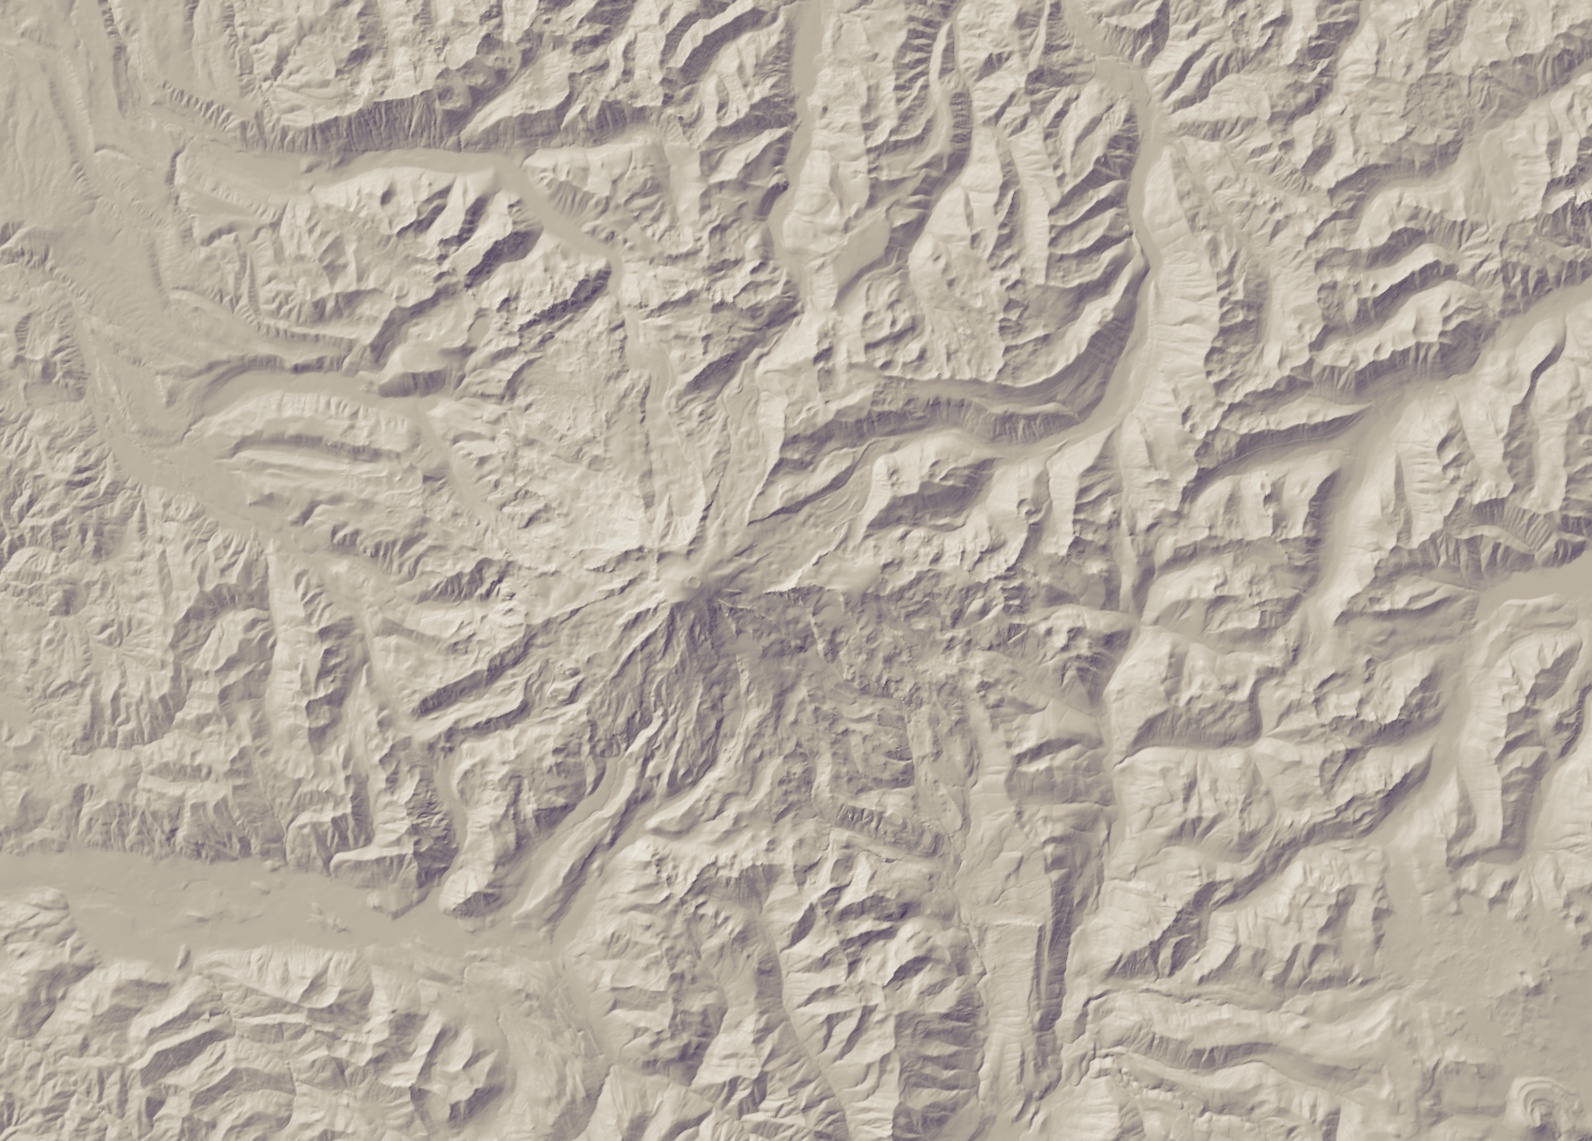
\includegraphics[width=1.0\linewidth]{Etat_de_l_art/terrain_diffuse.jpg}
 \caption{Ombrage classique}
 \end{subfigure}%
 ~
 \hspace{.05\textwidth}
 \begin{subfigure}[t]{0.47\textwidth}
 \centering
 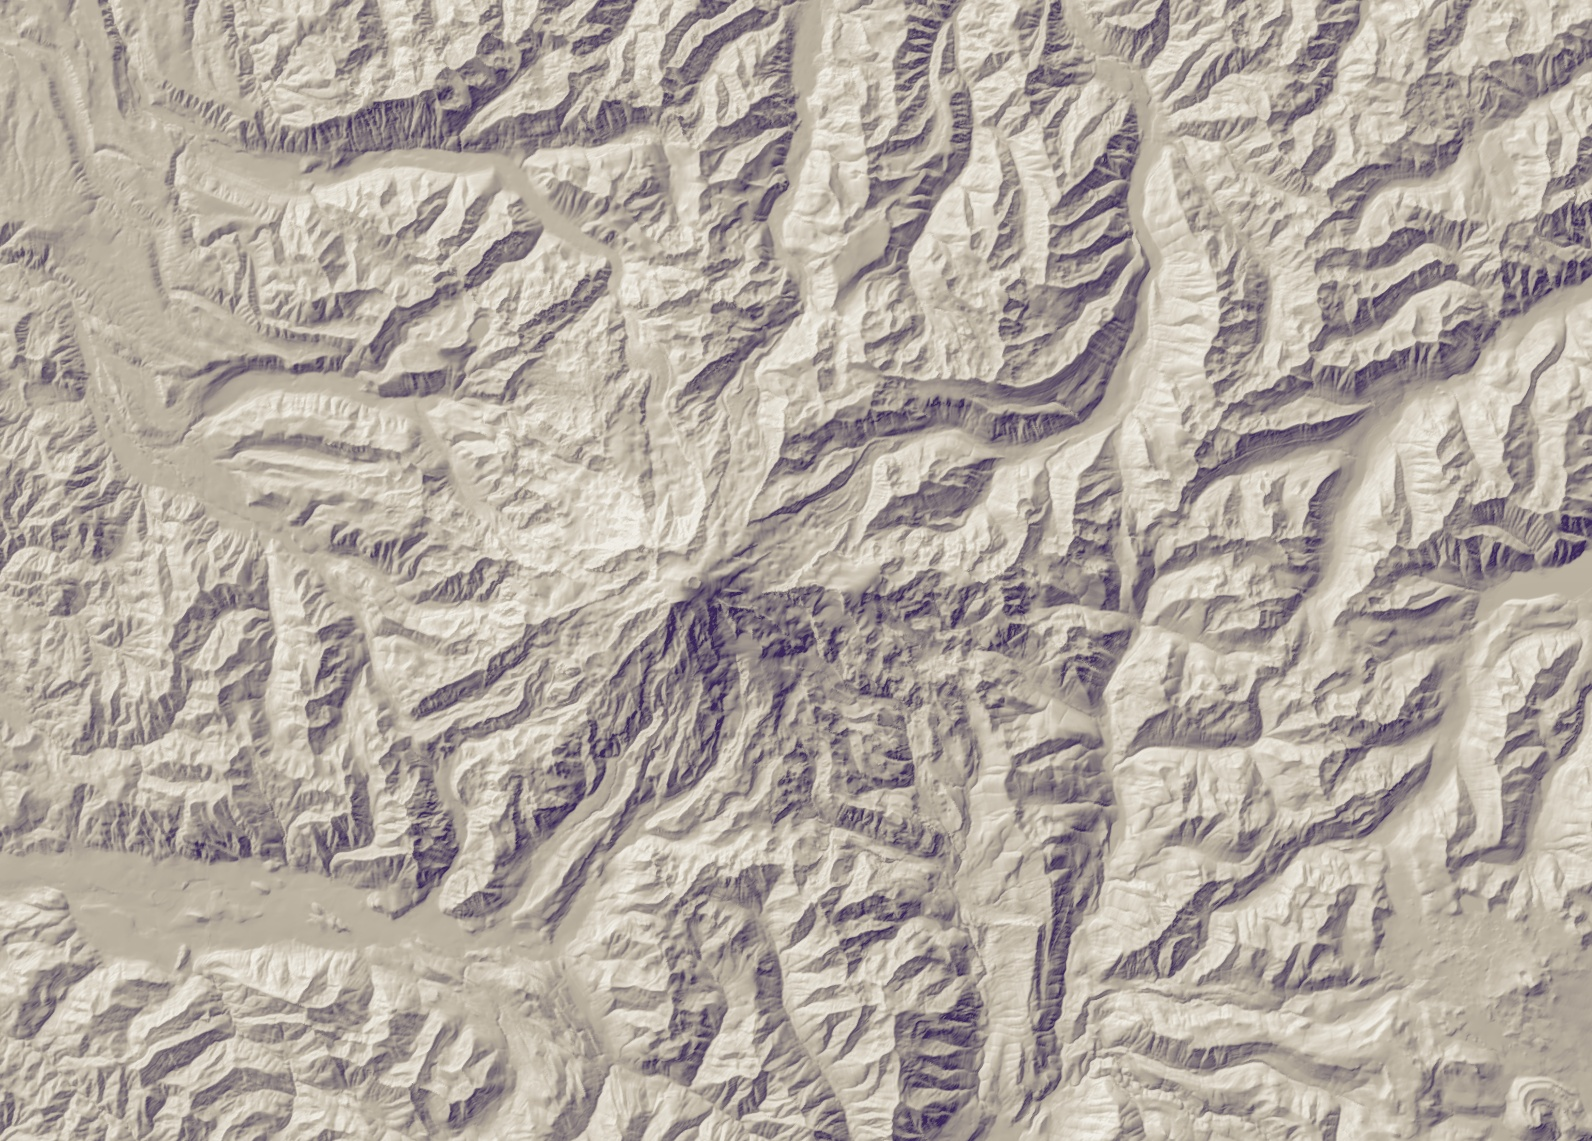
\includegraphics[width=1.0\linewidth]{Etat_de_l_art/terrain_exag.jpg}
 \caption{\textit{Exagerated Shading}}
 \end{subfigure}
 \caption{\label{fig:exageratedShading} Méthode de l'\textit{Exagerated Shading} sur un terrain montagneux}
\end{figure*}

Le principal inconvénient avec cette technique c'est qu'elle donne un effet bas-relief au rendu. Notre solution est inspirée de leur approche mais plus adaptée à un format panorama. 


\paragraph*{La Couleur} Une fois l'intensité de l'ombrage connue, il faut une méthode pour la dessiner. La technique la plus classique est de simplement multiplier cette intensité par la couleur de l'objet. Une approche plus complète serait d'utiliser une technique dite de "mélange" comme par exemple celle utilisée par Bousseau et al. \cite{bousseau2006interactive}  pour faire une rendu type aquarelle qui introduit notamment une fonction pour étendre une couleur sur une rampe  à l'aide d'une intensité (Fig. \ref{fig:watercolorschema}).
Une autre approche est d'associer cette intensité à une texture 1D de couleur. Cette texture peut être continue ou discontinue (technique du \textit{cel-shading}) permettant d'obtenir des contours très marqués et de donner un aspect "cartoon". 

Pour étendre le degré de contrôle du rendu de l'ombrage Barla et al. \cite{barla2006x} proposent d'utiliser une texture 2D dont l’abscisse donne la couleur correspondant à une intensité donnée (comme pour la texture de couleur 1D) et dont l'ordonnée peut être liée à n’importe quel autre paramètre de la scène (Fig. \ref{fig:xtoontexture}). Une telle approche pourrait permettre de prendre en compte par exemple la distance au point de vue ou l'altitude dans un rendu de panorama.

\begin{figure}[h!]
    \begin{minipage}[b]{0.4\linewidth}
        \centering 
        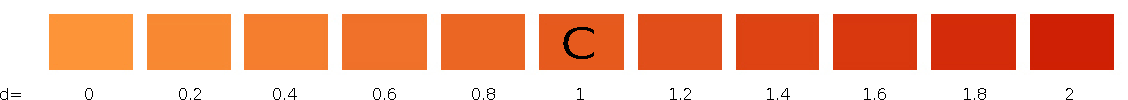
\includegraphics[width=1.0\linewidth]{Etat_de_l_art/watercolor.pdf}
        \caption{\label{fig:watercolorschema} Éclaircissement et assombrissement de la couleur $C$ (ici $(0.90,0.35,0.12)$) en utilisant le paramètre de densité $d$ \cite{bousseau2006interactive}.}

    \end{minipage}\hfill
    \begin{minipage}[b]{0.40\linewidth}
        \centering 
        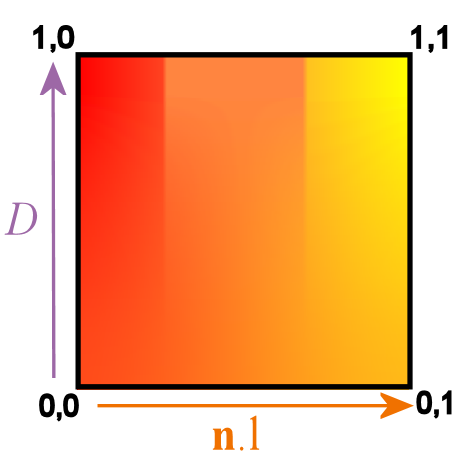
\includegraphics[width=0.5\linewidth]{Etat_de_l_art/xToon.png}
 		\caption{\label{fig:xtoontexture} Une texture 2D avec $l.n$ en paramètre principal et $D$ comme paramètre secondaire \cite{barla2006x}. }
    \end{minipage}
\end{figure}





\chapter{Calcul d'un ombrage expressif pour les panoramas}

\section{Vue d'ensemble de la solution}

Notre objectif est de faire un rendu 3D temps réel des ombres d'un panorama dans le style de l'atelier Novat. Comme vu dans l'étude du style de Pierre Novat, les ombres jouent un grand rôle dans lecture du panorama et mettent en valeur la forme de la montagne. Pour correspondre à ce style, notre rendu des ombres doit donner à voir le maximum de variation dans le terrain et ainsi améliorer la perception des formes de la montagne par l'utilisateur. En d'autres termes, lorsque le terrain est lisse, il faut voir que c'est plat et lorsqu'il y a des variations dans le terrain, petites ou grandes, il faut pouvoir les voir sans pour autant en rajouter artificiellement. Ces variations nous les appellerons aspérités.


Pour pouvoir construire notre modèle d'ombrage, nous nous appuyons sur un ensemble de règles qui résultent de nos études sur la cartographie et les œuvres de l'atelier Novat :

\begin{enumerate}
\item La lisibilité est privilégiée par rapport à la cohérence. 
\item La lumière a une direction générale qui vient d'en haut, à droite ou à gauche, de l'image. 
\item La direction peut être ajustée localement pour avoir une meilleure illumination de la zone.
\item Quand les ombres sont générées en utilisant un ordinateur, Tom Patterson conseille de faire deux ombrages différents puis de les fusionner pour garder le meilleur des deux. 
\item Les ombres portées sont moins présentes que l'ombrage.
\item Il n'y a pas de réflexion spéculaire.
\end{enumerate}

L'intuition derrière notre solution est la suivante : une fois une direction générale de la lumière choisie par l'utilisateur, nous la corrigeons localement afin de donner à voir au mieux les aspérités. Pour cela nous proposons de faire en sorte que chaque aspérité ait une face éclairée et une face à l'ombre tout en conservant l'orientation générale de la lumière, c'est-à-dire que la face en lumière doit rester du coté de la lumière principale. Pour appliquer cette correction, nous nous occupons uniquement d'ajuster l'azimut (c'est à dire l'orientation de la lumière par rapport au Nord). et nous ne touchons pas à l'élévation. Nous obtenons ainsi un ombrage localement ajusté et globalement cohérent. 
Cependant, comme les aspérités se répartissent sur plusieurs échelles : les petites aspérités se confondent avec les plus grandes et se mélangent, nous suivons la règle (4.) et proposons d'utiliser deux échelles sur lesquelles nous calculons deux ombrages que nous fusionnons pour obtenir l'ombrage final. Enfin nous ajoutons une couche d'ombres portées plus discrète qui souligne le relief global.

En pratique nous prenons en entrée une carte de hauteur (modèle numérique de terrain) et nous travaillons en espace image, le terrain vu de dessus étant dans le plan $xy$.



\section{L'orientation de la lumière}



Notre modèle d'illumination est le modèle Lambertien. Le calcul de l'ombrage s'obtient par le produit scalaire entre un vecteur de lumière $\vec{l}$ et la normale $\vec{n}$ de la surface courante :
\begin{equation} 
D = \vec{l}\cdot{\vec{n}}\end{equation}

Pour améliorer la perception de la forme, nous modifions localement la direction de la lumière pour s’assurer de voir toutes les aspérités. En plaçant la lumière perpendiculairement à la pente , nous nous assurons de toujours produire une zone ombrée et une zone éclairée (Fig. \ref{fig:correction}). 
\begin{figure}[!h]
\centering 
        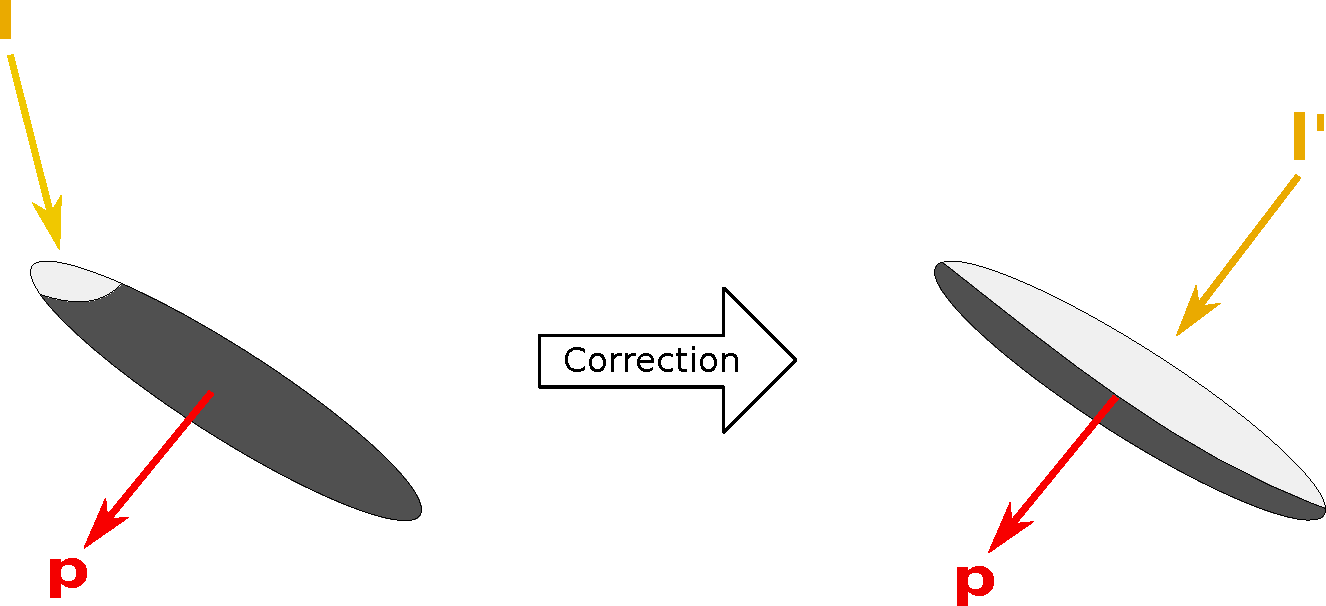
\includegraphics[width=0.4\linewidth]{Solution/correction_light.pdf}
        \caption{\label{fig:correction} Correction local sur un galet de la lumière $\vec{l}$ à l'aide de la pente $\vec{p}$ }
\end{figure}
%\jhon{C'est l'}
Notre problématique est donc de corriger l'azimut de $\vec{l}$ qui est sa projection sur le plan $xy$ que nous appellerons $\vec{l}_a$. En définissant le vecteur lumière par ses coordonnées polaires, les deux angles d'Euler : $\alpha$ et $\gamma$ (Fig. \ref{fig:euler}), la question revient à appliquer une correction $\theta$ à l'angle $\alpha$ locale en fonction d'une direction principale, tout en conservant $\gamma$. Cette direction principale est la pente $\vec{p}$ qui est définie par le gradient de la carte de hauteur, en d'autre terme, la normale projetée sur le plan $xy$. Donc nous calculons l'angle $\theta$ entre l'azimut du vecteur lumière $\vec{l}_a$ et la pente $\vec{p}$, pour l'appliquer ensuite à $\alpha$ et recalculer un vecteur lumière local $\vec{l'}$


\begin{figure}[!h]
\centering 
        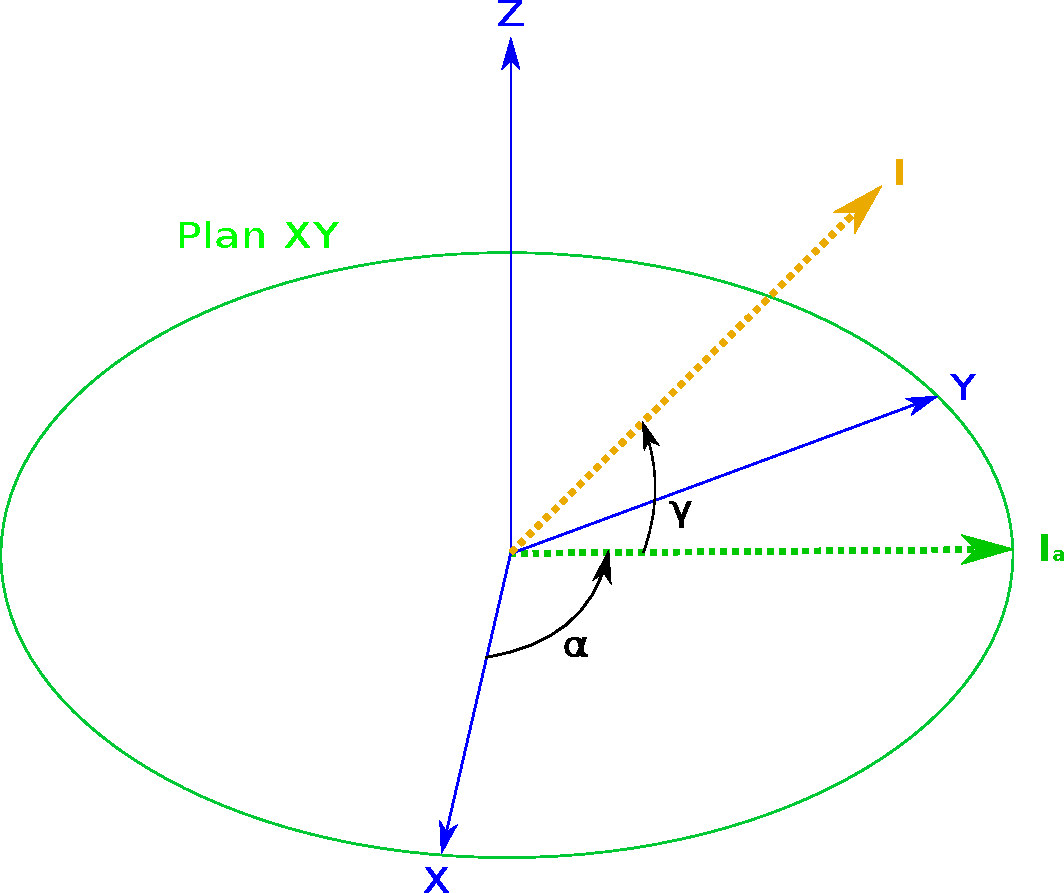
\includegraphics[width=0.3\linewidth]{Solution/euler_V3.pdf}
        \caption{\label{fig:euler} Angles d'Euler du vecteur lumière $\vec{l}$ avec $\vec{l}_a$ sa projection sur le plan $xy$ }
\end{figure}

Dans un 1er temps, nous cherchons à aligner parfaitement la lumière $\vec{l}$ avec la pente $\vec{p}$ , mais nous voulons aussi garder une cohérence globale c'est à dire que nous ne voulons pas que la direction de $\vec{l}$ se renverse totalement . Pour cela nous calculons  $\widehat{\vec{l}_a,\vec{q}}$ avec $\vec{q}$ la pente signée dans le sens de la lumière. Ainsi nous nous assurons que $\widehat{\vec{l}_a,\vec{q}}$ soit $\leq \pi $ :
\begin{equation}
\label{equationReverseN}
\vec{q} = 
	\left\{
    \begin{array}{ll}
        -\vec{p} & \mbox{si } \widehat{\vec{l}_a,\vec{p}} \leq \pi\\
		\vec{p} & \mbox{sinon}				
    \end{array}
\right.
\end{equation}


Ensuite nous calculons l'angle $\theta$ entre $\vec{l}_a$ et $\vec{q}$ en signant avec le déterminant $\Delta$ pour que $\theta$ soit dans l'intervalle  $-\frac{\pi}{2}$ et $\frac{\pi}{2}$ :
\begin{equation}
\label{equationAngleOri}
 \theta = \frac{\Delta}{|\Delta|} \arccos( \vec{l}_a \cdot{\vec{q}}) \ 
 \mathrm{avec} \  
\Delta =  \vec{l_{a_x}}\vec{q_y} - \vec{l_{a_y}}\vec{q_x}
\end{equation}

Enfin nous pouvons reconstruire le vecteur lumière ajusté localement grâce à une matrice de rotation :
\begin{equation}
\label{equationRotationMat}
\vec{l'} = 
\begin{pmatrix}
x \\
y \\
z \\
\end{pmatrix}
=
\begin{pmatrix}
\cos \gamma  \cos \alpha + \theta\\
\sin \gamma \\
\cos \gamma  \sin \alpha + \theta \\
\end{pmatrix}
\end{equation}



\begin{figure*}[h!]
\centering
 \begin{subfigure}[t]{0.47\textwidth}
 \centering
 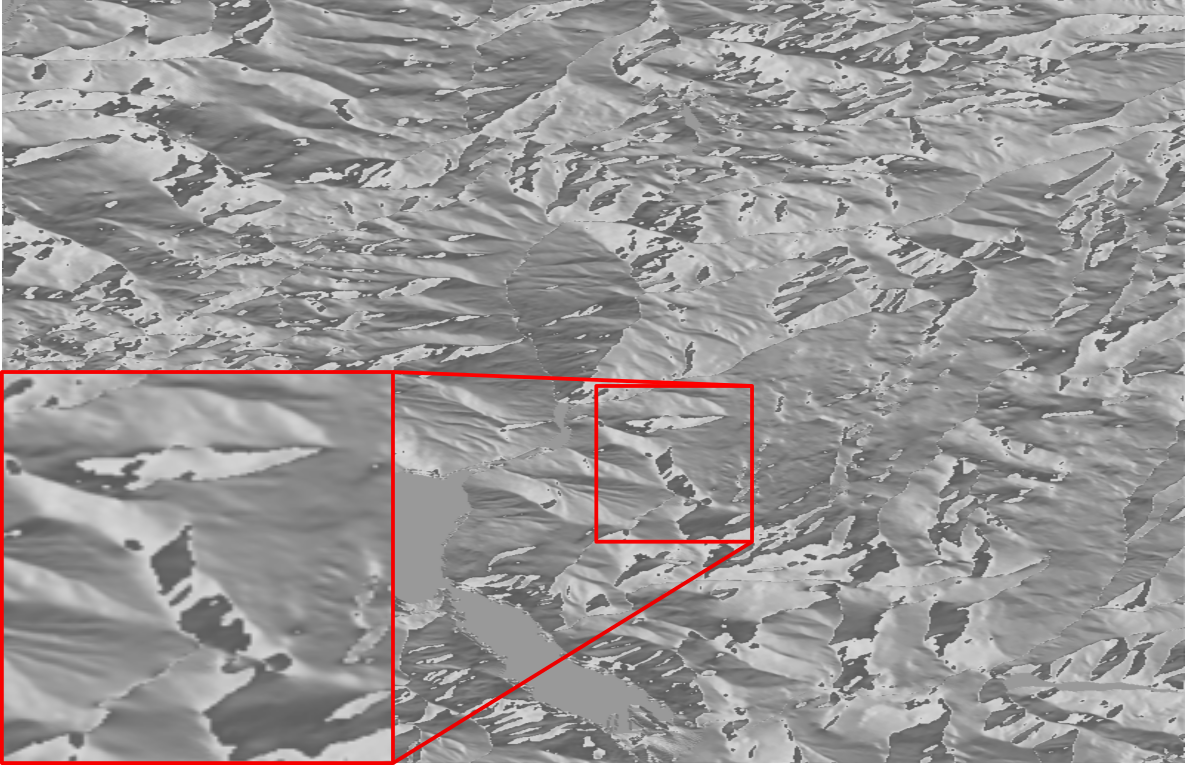
\includegraphics[width=1.0\linewidth]{Solution/theta_discontinu.png}
 \caption{$\theta$ en niveau de gris}
 \end{subfigure}
 \begin{subfigure}[t]{0.47\textwidth}
 \centering
 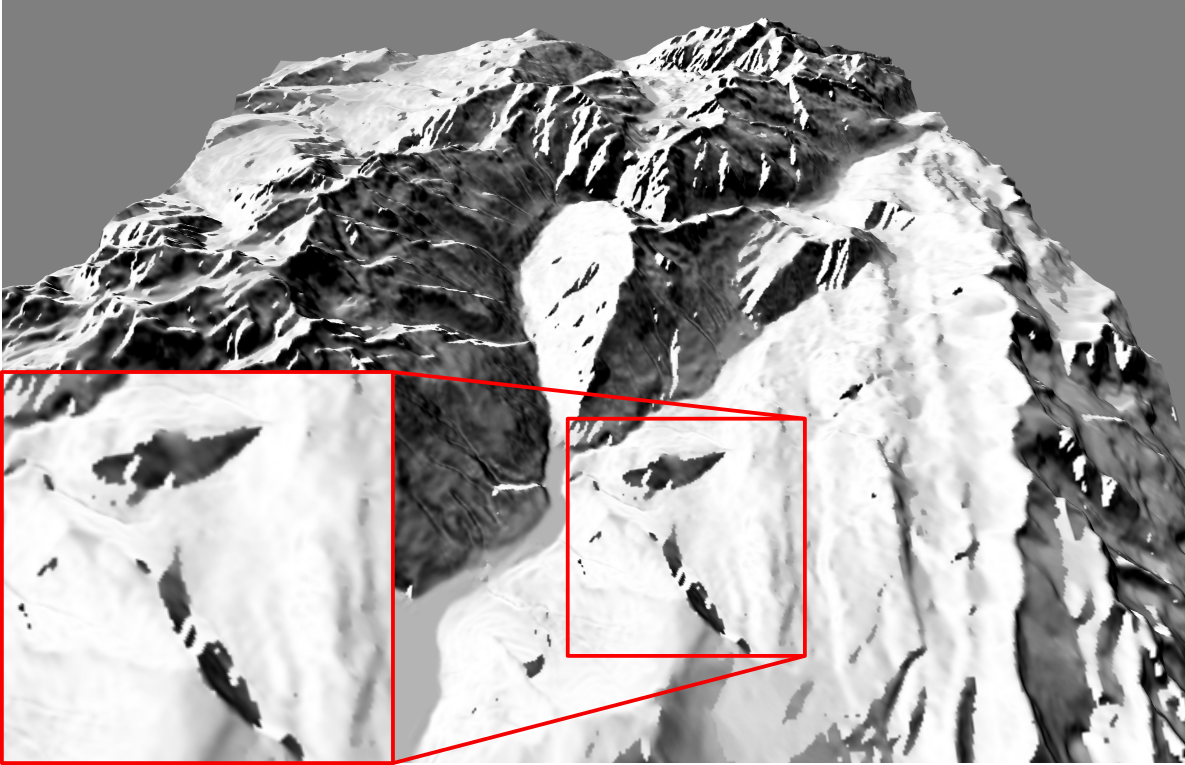
\includegraphics[width=1.0\linewidth]{Solution/ombrage_discontinue.png}
 \caption{Ombrage avec correction de la lumière}
 \end{subfigure}
 \caption{\label{fig:shadingDiscontinu}Exemple de correction de la lumière sur un terrain ($\alpha = 45\degres$ (Nord-Ouest), $\gamma = 45 \degres$) . Nous constatons que la lumière s’aligne bien avec les aspérité mais aux prix de discontinuité. }
\end{figure*}





À ce stade, comme nous pouvons le constater sur la Figure \ref{fig:shadingDiscontinu}, il y a des discontinuités dans le vecteur lumière qui ont deux causes differentes :
\begin{enumerate}
\item $\theta$ passe d'un seul coup de $-\frac{\pi}{2}$ à $\frac{\pi}{2}$ et inversement  
\item Quand $\vec{p'}$ est nul, il est possible que ses voisins soit très petits mais pas dans le même sens. 
\end{enumerate}

Pour corriger la première discontinuité nous multiplions $\theta$ avec une interpolation d’Hermite qui va permettre d'interpoler $\theta$ de manière continue  entre $-\frac{\pi}{2}$ et $\frac{\pi}{2}$. Cette interpolation se fait en deux étapes. 

Dans un premier temps nous calculons $S(x)$ qui va limiter la valeur de $|\theta|$ entre $T$ et $\frac{\pi}{2}$ et inverser cet intervalle. C'est-à-dire que lorsque de $|\theta|$ $\leq T$, alors l'interpolation nous renvoie :
\begin{equation}
\label{equationClamp}
S(x) = 
	\left\{
    \begin{array}{ll}
        0 & \mbox{si } x \leq 0 \\
		x & \mbox{si } 0 \leq x \leq 1 \\
        1 & \mbox{si } 1 \leq x \\
    \end{array}
\right.
\mathrm{avec} \  
x = - \frac{|\theta| - T}{\frac{\pi}{2}-T} + 1 
\end{equation}

Note : $T$ est une limite laissée au choix de l'utilisateur, elle peut être entre $0$ et $\frac{\pi}{2}$ où à $0$, il n'y a aucune correction de lumière qui est faite et à $\frac{\pi}{2}$ la correction est maximale. Cependant pour le reste du rapport $T = \frac{\pi}{3}$ qui est le meilleur choix pour avoir une bonne correction sans avoir de discontinuité importante.


Ensuite, nous calculons le polynôme d'Hermite pour avoir un facteur continu entre $0$ et $1$ : 
\begin{equation}
\label{equationHermite}
H(x) = 3S(x)^2 - 2S(x)^3 
\end{equation}

Pour corriger la seconde discontinuité, nous utilisons simplement la norme de la projection de $\vec{n}$ sur le plan $xy$, c'est à dire $||\vec{p}||$.  Cela permet d’éviter d'avoir des faibles corrections lorsque la normale est presque verticale.
Ainsi nous ajoutons une étape entre  \eqref{equationAngleOri} et \eqref{equationRotationMat} :
\begin{equation}
\theta' = \theta \ . \ H(|\theta|) \ . \ ||\vec{p} ||
\end{equation}





\begin{figure*}[h!]
\centering
 \begin{subfigure}[t]{0.47\textwidth}
 \centering
 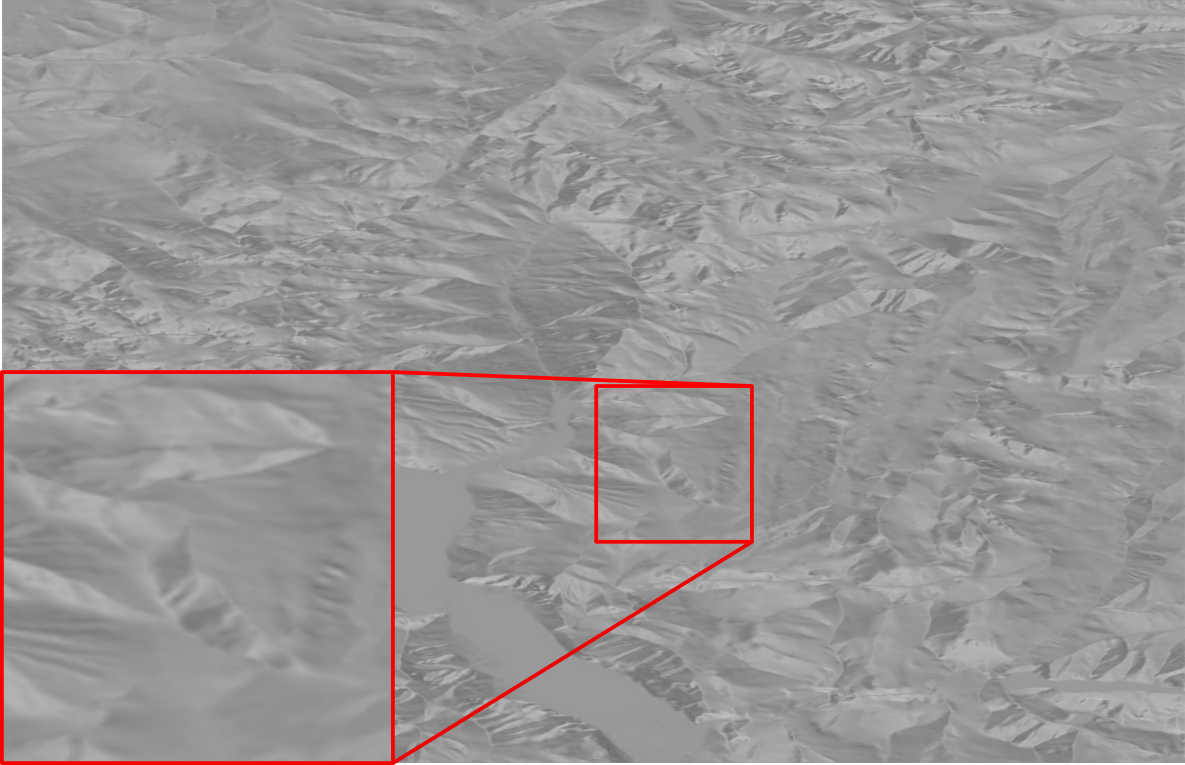
\includegraphics[width=1.0\linewidth]{Solution/theta_continu.png}
 \caption{$\theta$ en niveau de gris}
 \end{subfigure}
 \begin{subfigure}[t]{0.47\textwidth}
 \centering
 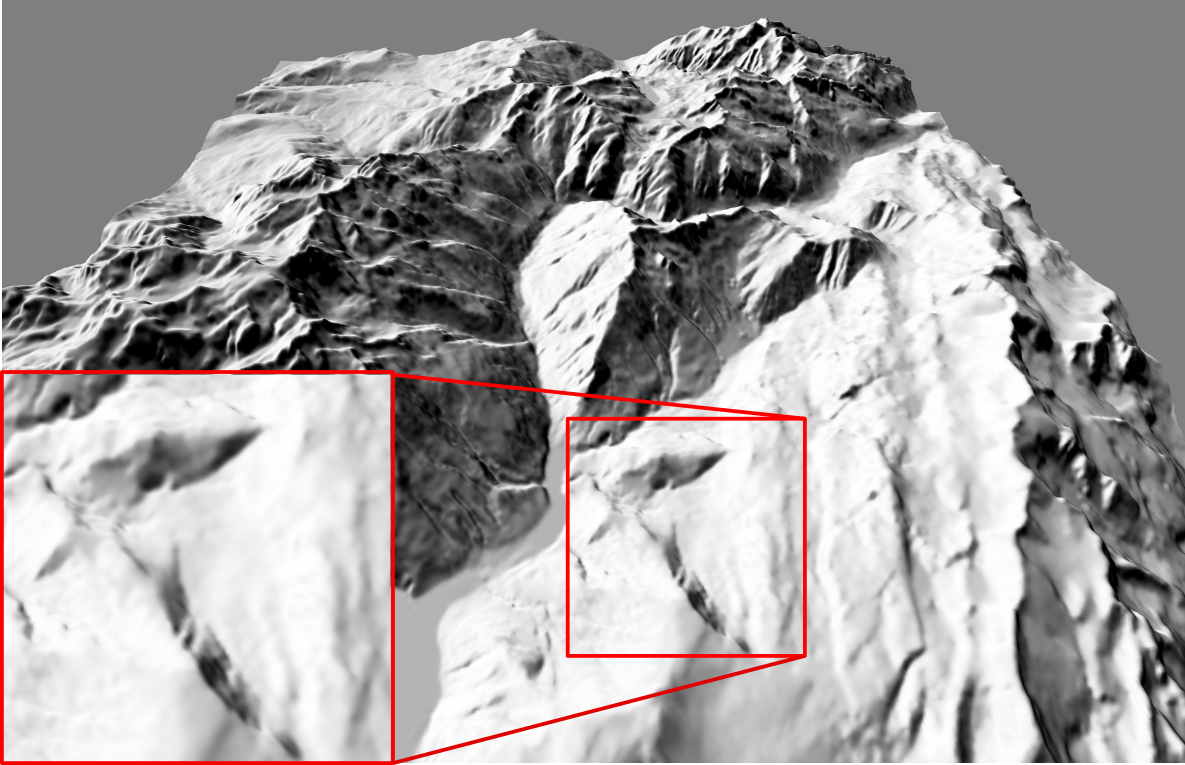
\includegraphics[width=1.0\linewidth]{Solution/ombrage_continue.png}
 \caption{Ombrage avec correction de la lumière}
 \end{subfigure}
 \caption{\label{fig:shadingContinu}Exemple de correction de la lumière sur un terrain sans les discontinuités ($\alpha =  45\degres$ (Nord-Ouest), $\gamma = 45\degres$). Le résultat est bien plus continue sans pour autant casser la correction.}
\end{figure*}


\section{L'ombrage multi échelle}

Une fois l'orientation locale de la lumière faite, il se pose un nouveau problème. En effet, nous alignons la lumière par rapport à la pente, or la direction de cette pente est majoritairement influencée par la forme de la montagne et non par les petites aspérités qui sont dessus. En d'autres termes, avec cette méthode nous obtenons des montagnes blanches d'un coté, sombres de l'autre sans pouvoir percevoir les petites aspérités. 
\begin{figure*}[h!]
 \begin{subfigure}[t]{0.47\textwidth}
 \centering
 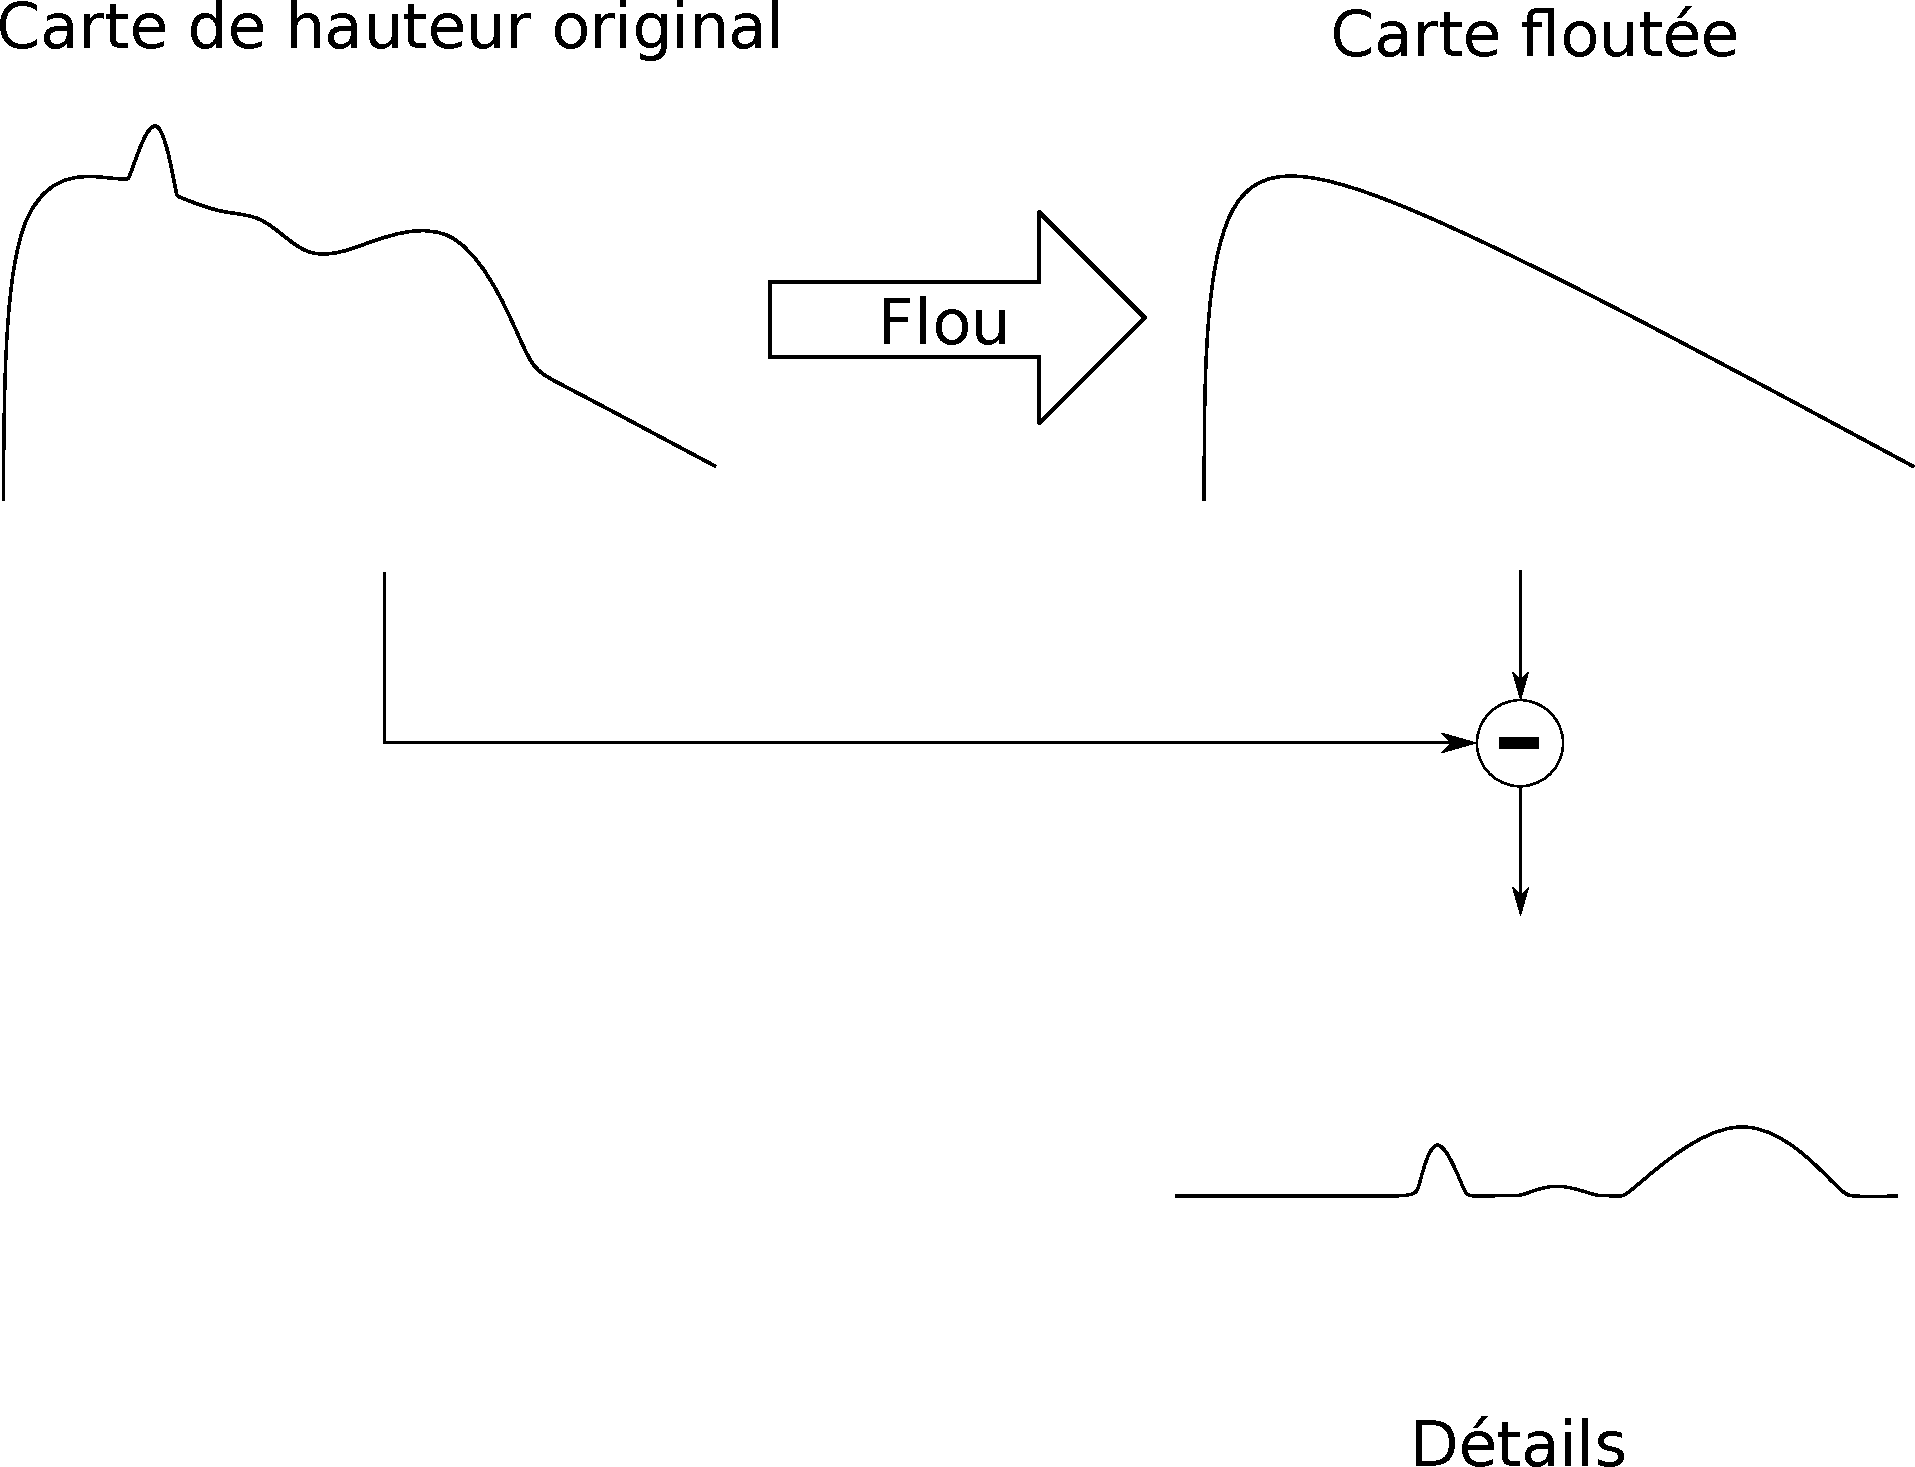
\includegraphics[width=1.0\linewidth]{Solution/pyramide_Laplace_schema.pdf}
 \caption{Une dimension}
 \end{subfigure}
   ~
 \hspace{.05\textwidth}
  \begin{subfigure}[t]{0.47\textwidth}
 \centering
 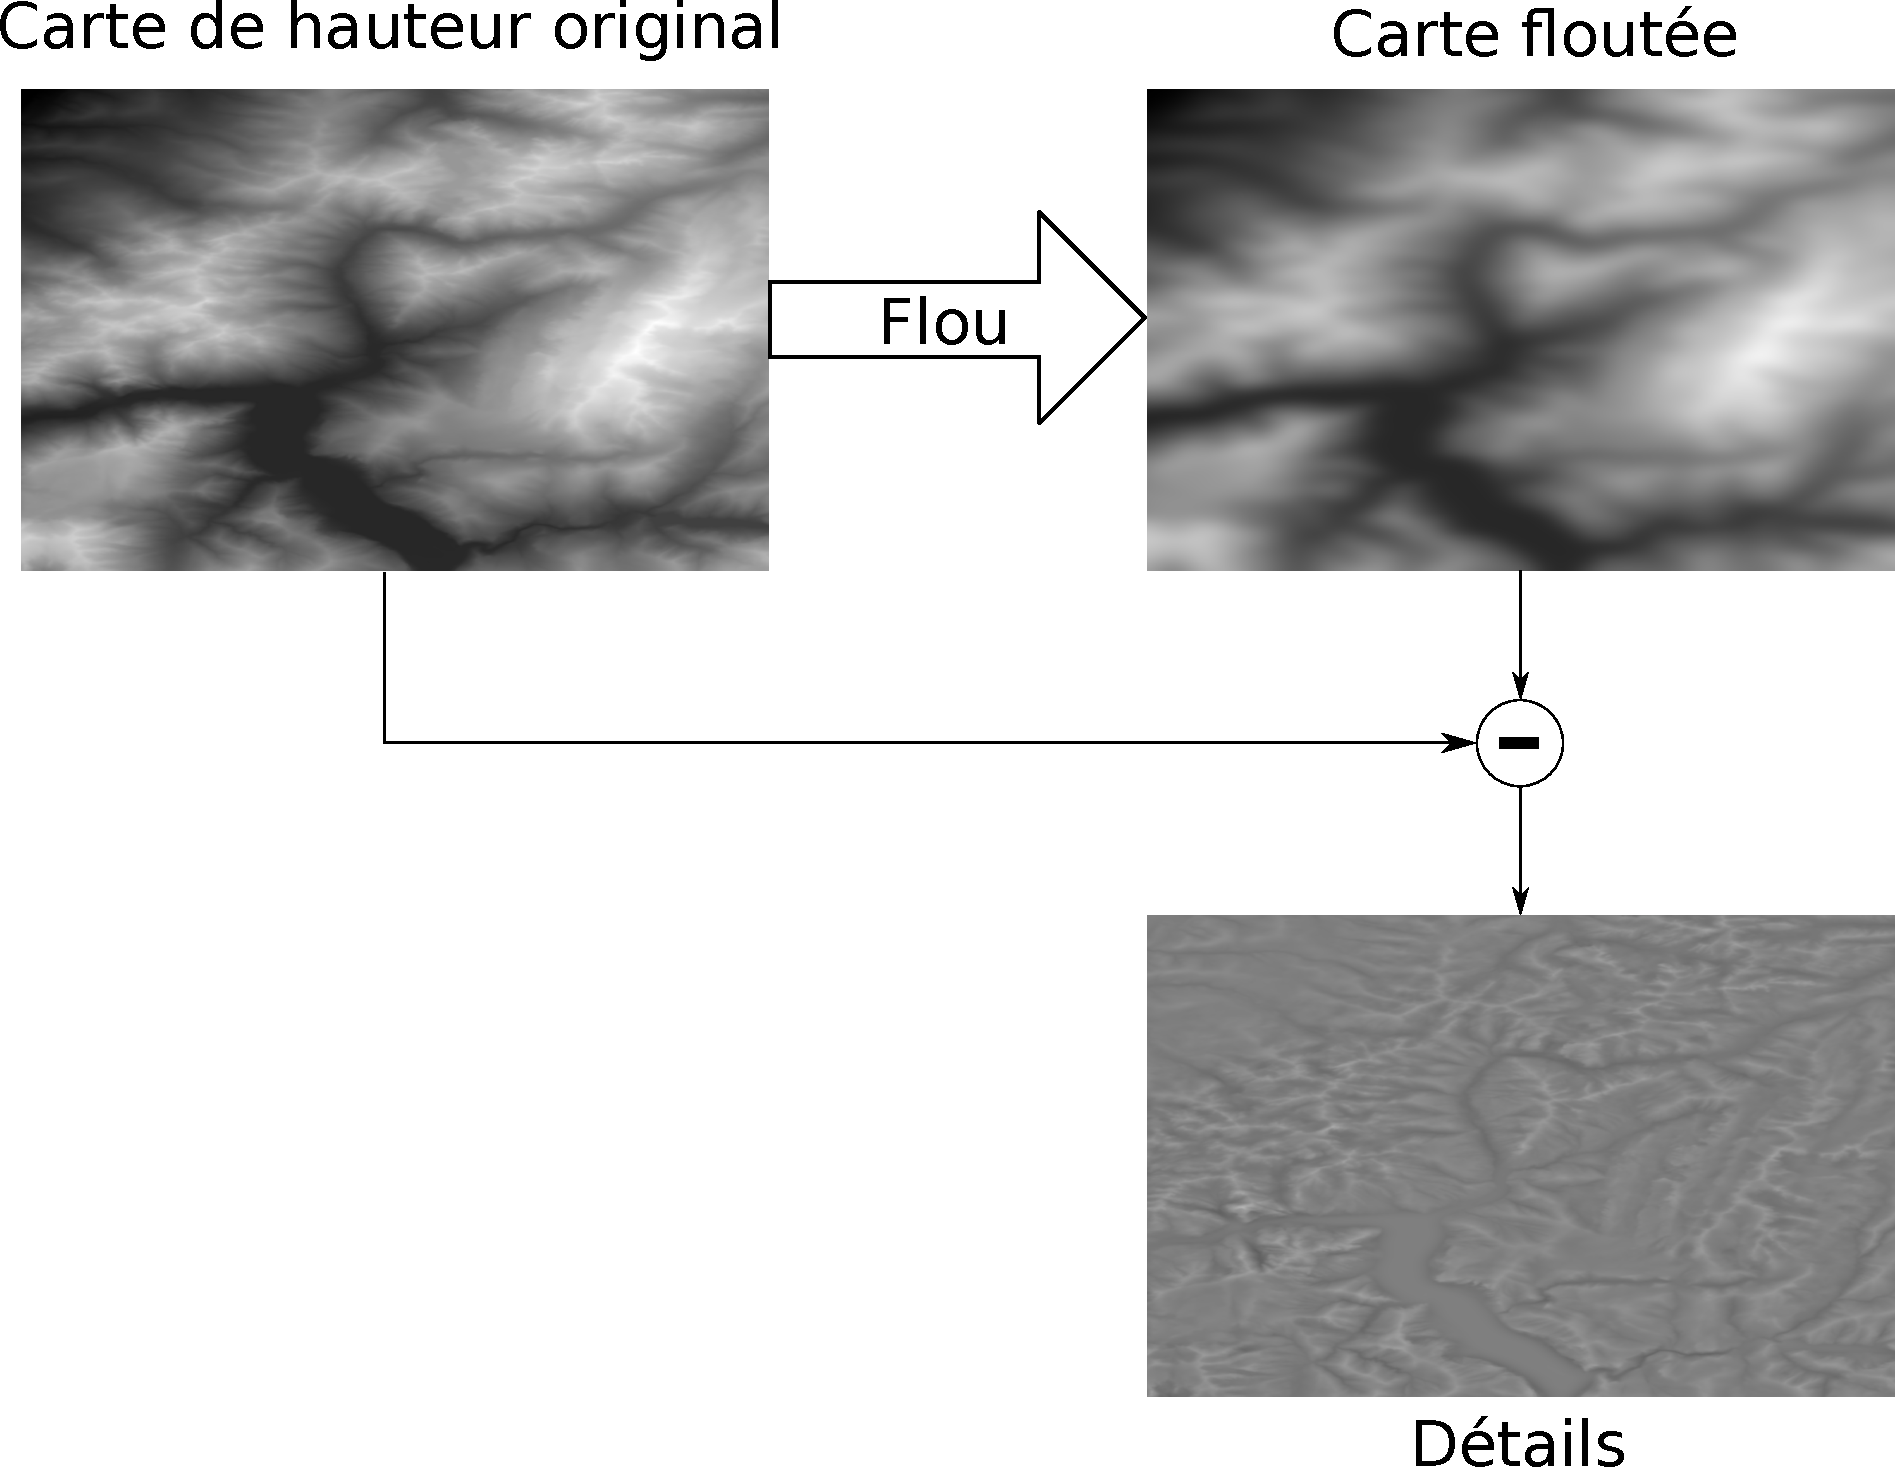
\includegraphics[width=1.0\linewidth]{Solution/pyramide_Laplace_image.pdf}
 \caption{Deux dimensions}
 \end{subfigure}
 \caption{\label{fig:pyramide} Pyramide Laplacienne sur une carte de hauteur}
\end{figure*}
La solution est donc d'utiliser un système multi-échelle pour permettre aux détails de ressortir. Notre solution consiste à utiliser une pyramide Laplacienne \cite{adelson1984pyramid} pour produire deux échelles. Le principe est de produire à l'aide d'un flou gaussien une version floutée de la carte de hauteur et ensuite de faire la différence entre la carte originale et la version floutée (Fig \ref{fig:pyramide})
Le flou gaussien s'obtient en convoluant chaque point de la carte de hauteurs par une gaussienne en deux dimensions : 
\begin{equation}
G(x,y,\sigma) = \frac{1}{2\pi\sigma^2}e^{-\frac{x^2+y^2}{2\sigma^2}},
\end{equation}
avec $x$ et $y$ la distance par rapport à l'origine et $\sigma$ l’écart type de la gaussienne.


\begin{figure}
\centering
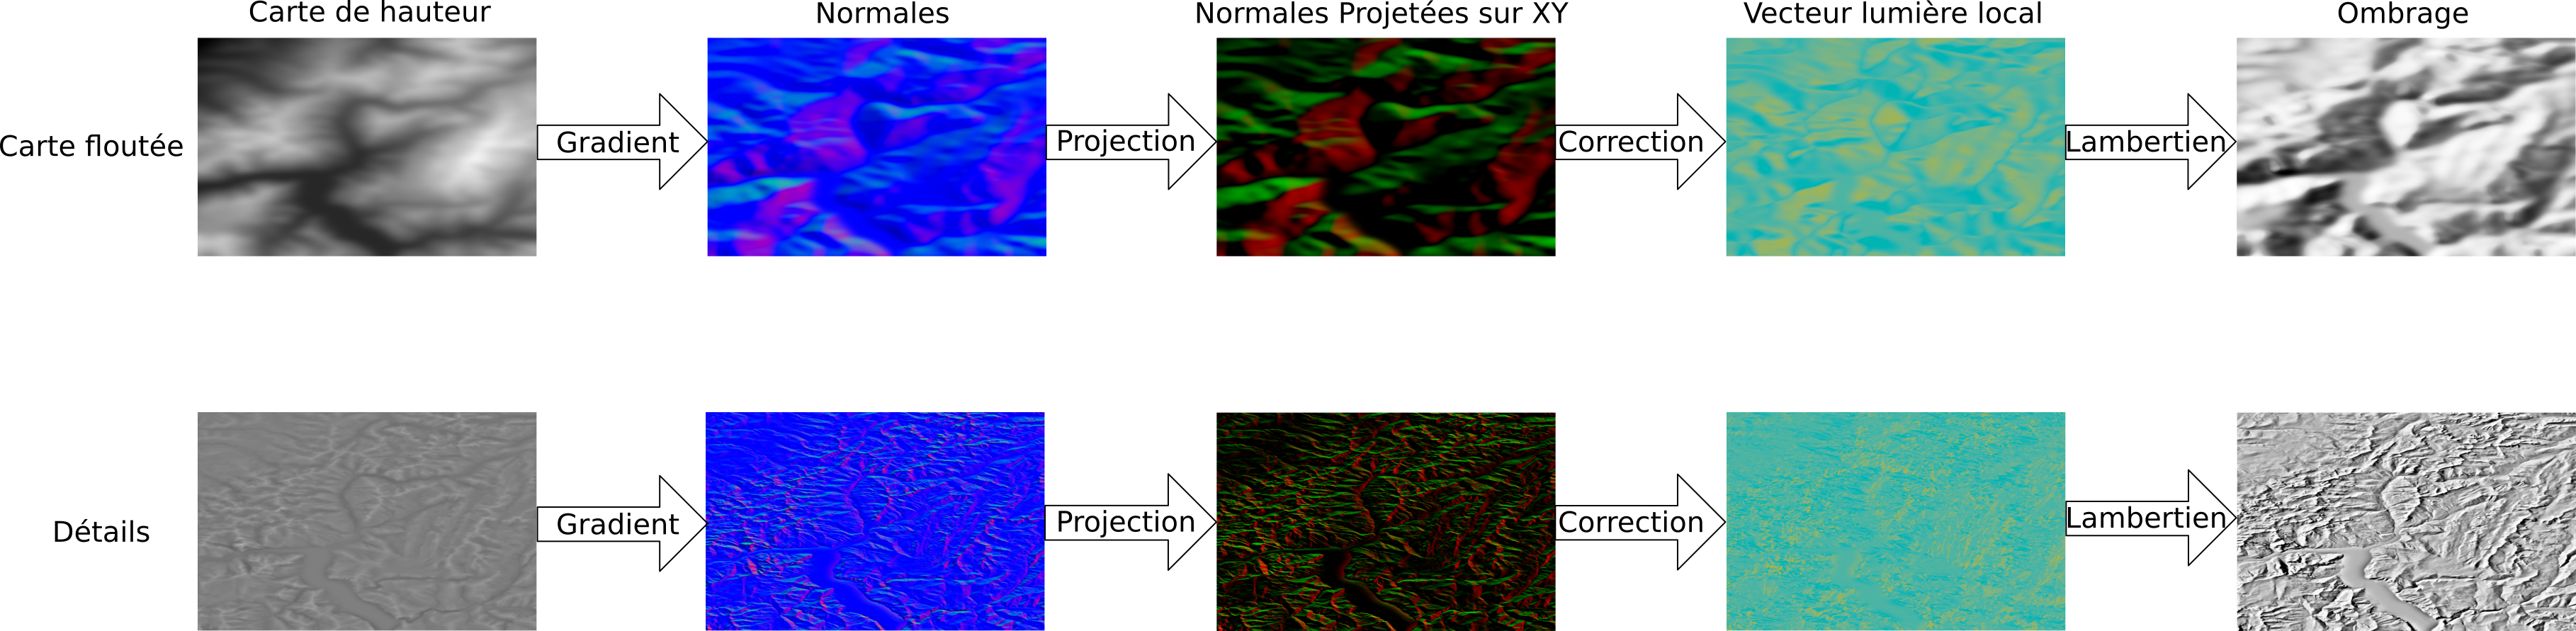
\includegraphics[width=1.0\linewidth]{Solution/pyramide_Laplace_image_extended.png}

\caption{\label{fig:pyramide_extended}Les différentes étapes de notre méthode pour générer l'ombrage sur deux échelles}
\end{figure}




Une fois ces deux échelles obtenues, nous extrayons les normales puis nous calculons l'orientation de la lumière localement de manière indépendante afin de calculer un ombrage. (Fig. \ref{fig:pyramide_extended}).  


\section{Fusion des ombrages}
Les deux ombrages de chaque échelles obtenues, il faut maintenant les fusionner afin d'obtenir un unique ombrage pour le rendu final. Cependant cette fusion n'est pas triviale. En effet, la manière de fusionner va influencer la quantité de détails perçus et le style final du rendu. Ainsi, une simple interpolation linéaire ne permet pas de répondre correctement à la problématique de percevoir la maximum de détails tout en gardant le contraste et la nervosité du style Novat. 

Parmi les fonctions de fusion qui existent, celles de type \textit{Overlay} répondent à notre problématique. L'idée principale de ces fonctions est de partir d'un niveau de gris compris entre 0 et 1 (dans notre cas, l'ombrage de la partie détaillée $d$) et de lui appliquer un $2^e$ niveau de gris (dans notre cas, l'ombrage de la partie floutée $f$) pour faire faire varier le $1^{er}$ niveau de gris. Ça a pour avantage d'avoir un niveau de gris principal et un secondaire. Nous utilisons celle utilisée dans le rendu d'aquarelle de Bousseau et al. \cite{bousseau2006interactive} (équation  \ref{equationAquarelle} et Fig. \ref{fig:watercolorcurve}) qui a pour avantage de n'enlever aucune aspérité tout en augmentant le contraste de l'ombrage (cf Fig. \ref{fig:comparaisonFusion}).
\begin{equation}
\label{equationAquarelle}
        A(d,f) = d - (d -d^2)( 1-2f) 
\end{equation}
\begin{figure}[h!]
\centering
        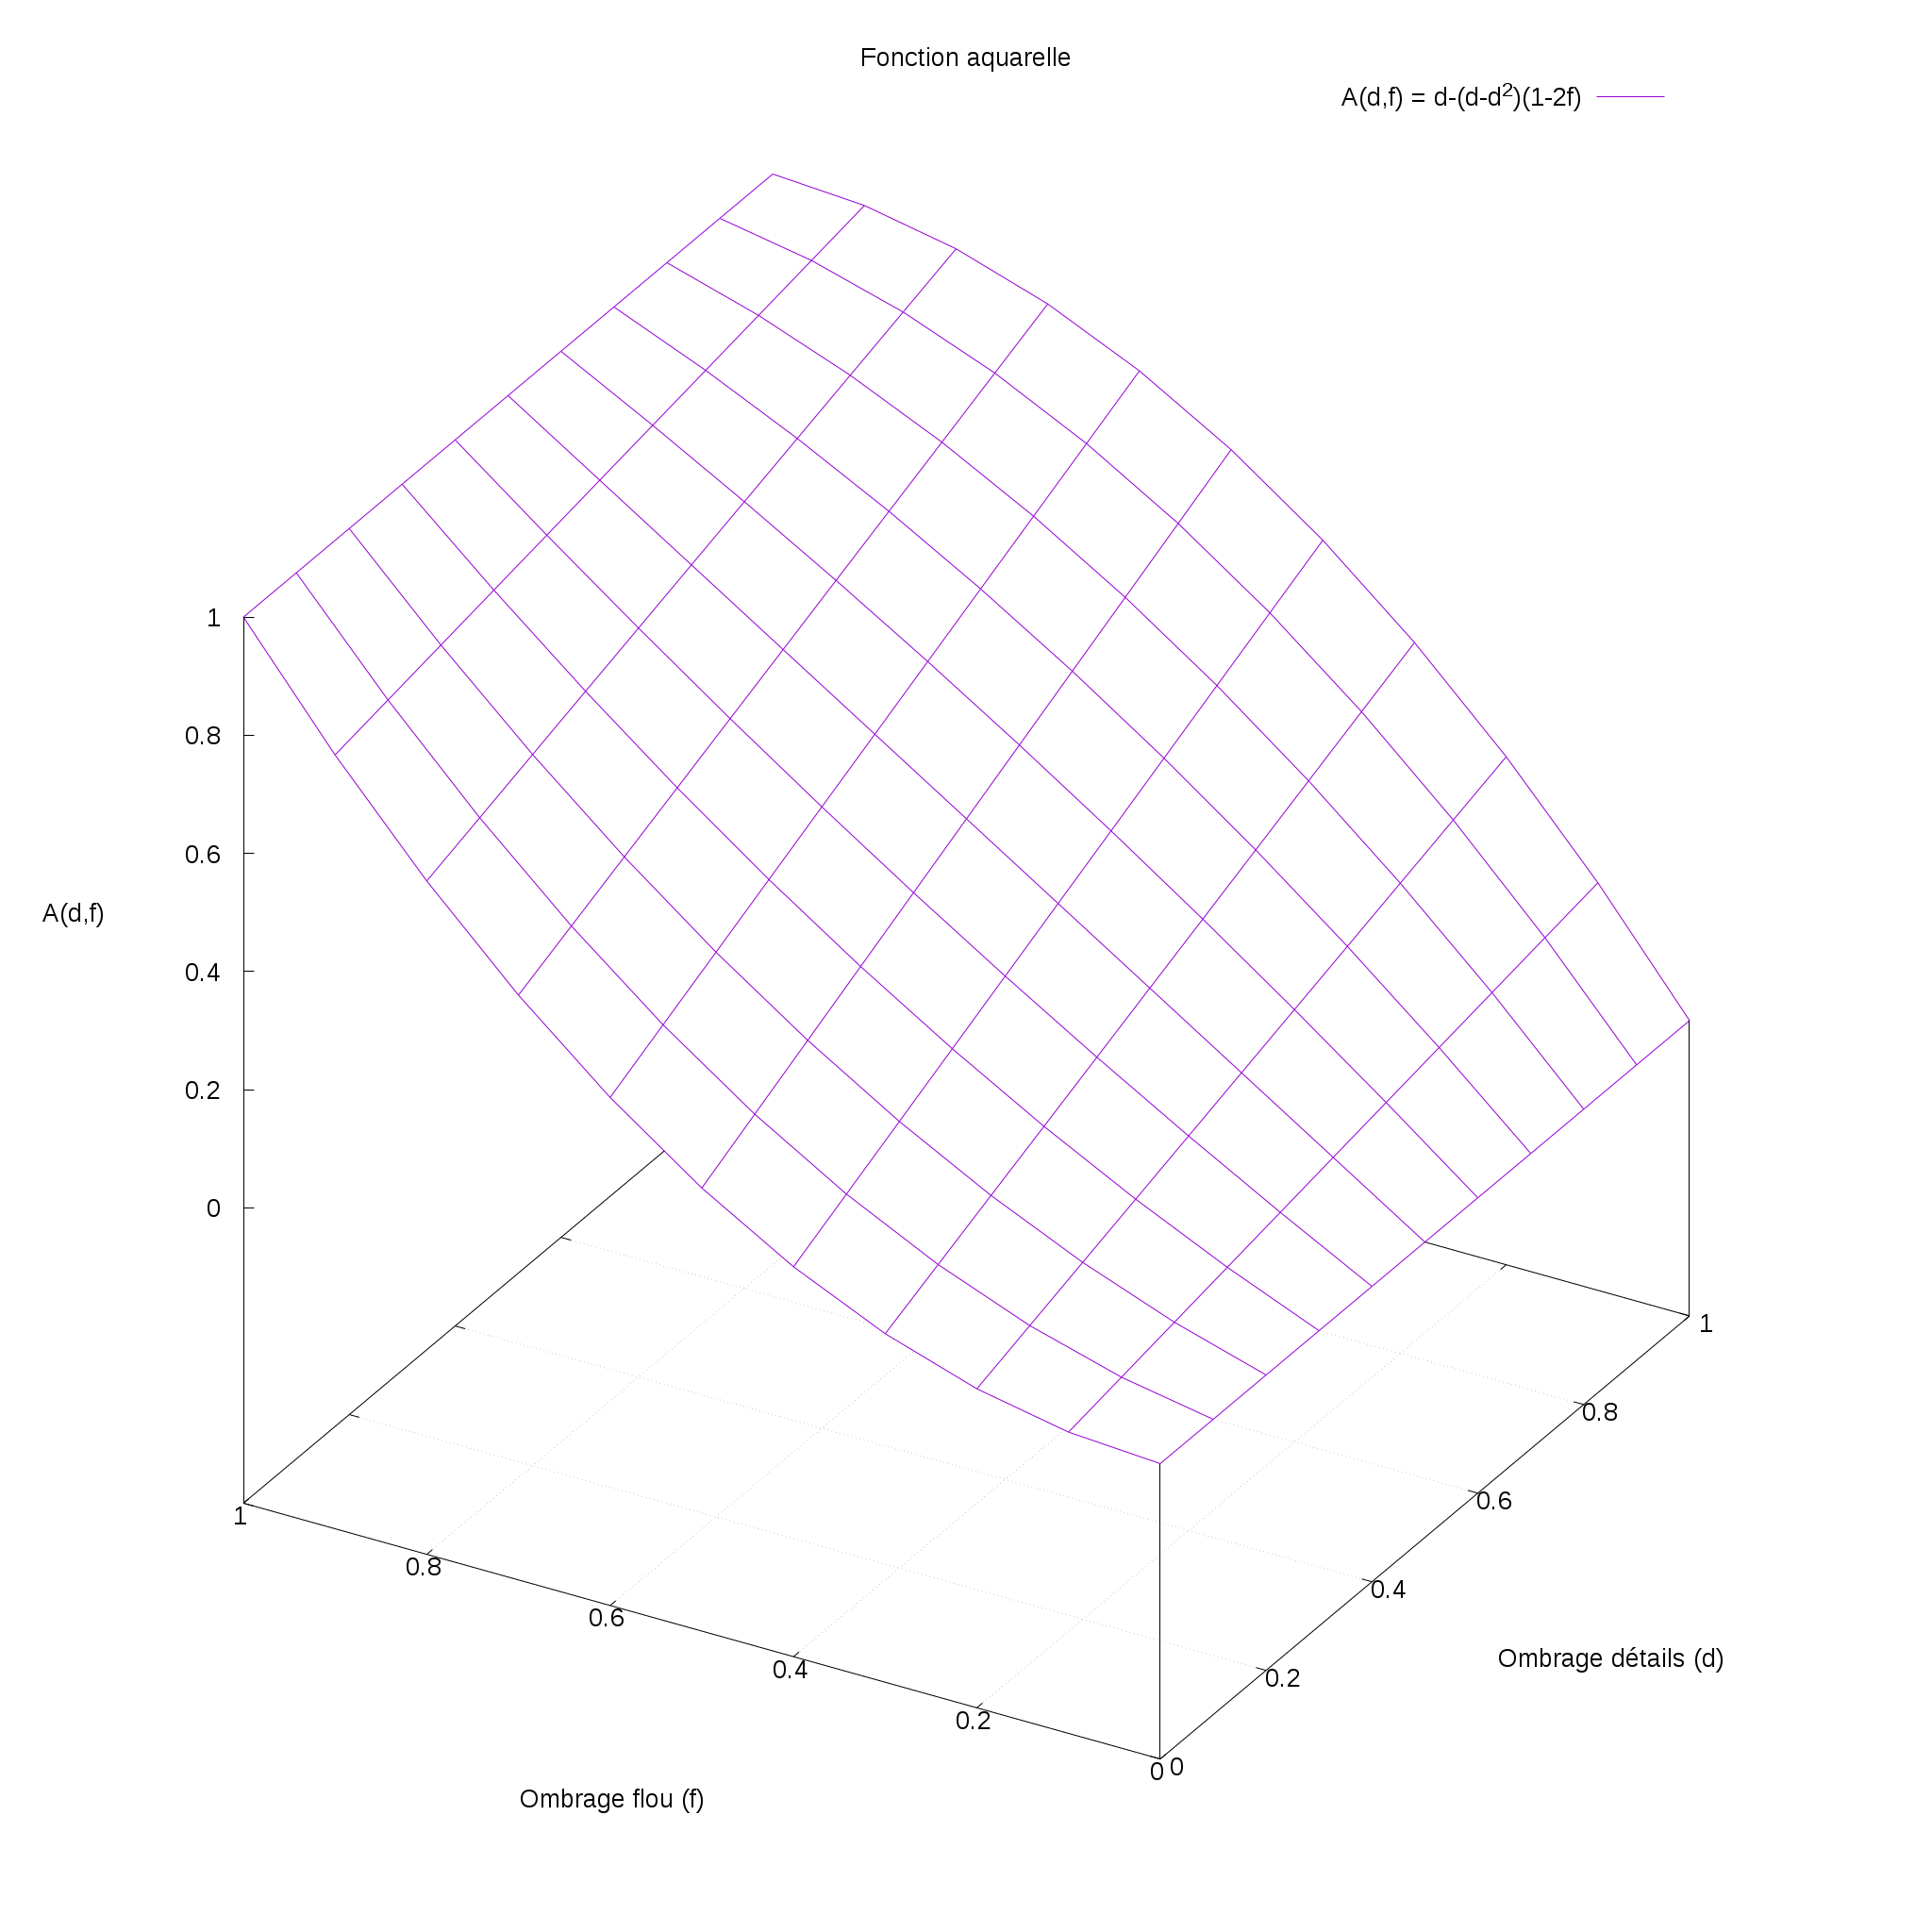
\includegraphics[width=0.5\linewidth]{Solution/watercolor_curve}
        \caption{\label{fig:watercolorcurve} Courbe de la fonction $A(d,f)$}

\end{figure}

\begin{figure*}[!h]
\centering
 \begin{subfigure}[t]{0.32\linewidth}
 \centering
 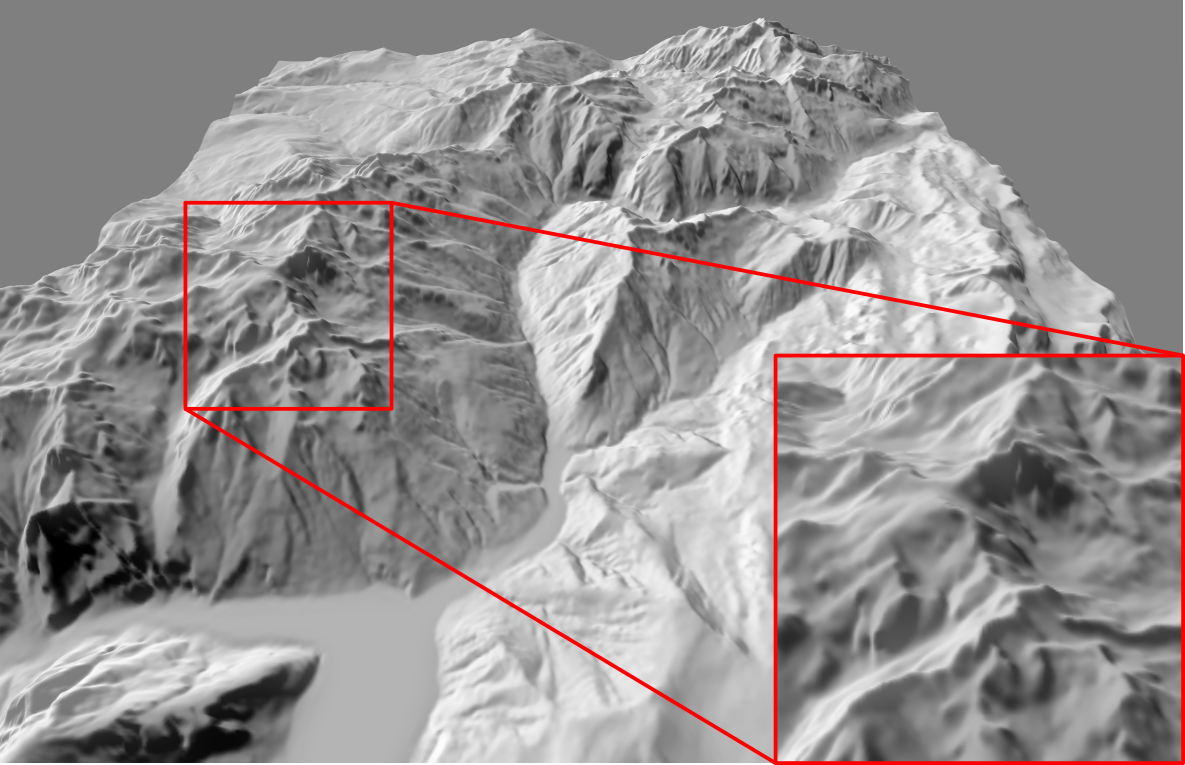
\includegraphics[width=1.0\linewidth]{Solution/ShadeLineaire.png}
 \caption{Interpolation linéaire }
 \end{subfigure}
 \begin{subfigure}[t]{0.32\linewidth}
 \centering
 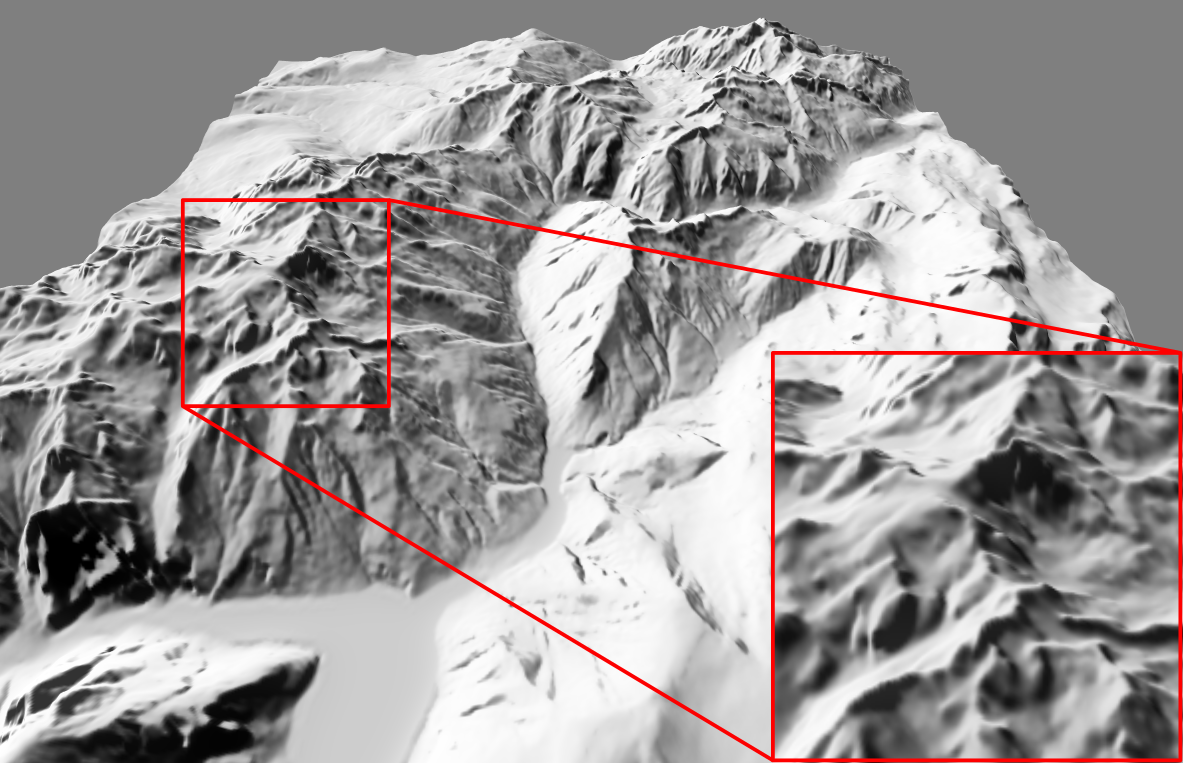
\includegraphics[width=1.0\linewidth]{Solution/ShadeOverlay.png}
  \caption{Overlay de Gimp et photoshop }
 \end{subfigure}
  \begin{subfigure}[t]{0.32\linewidth}
 \centering
 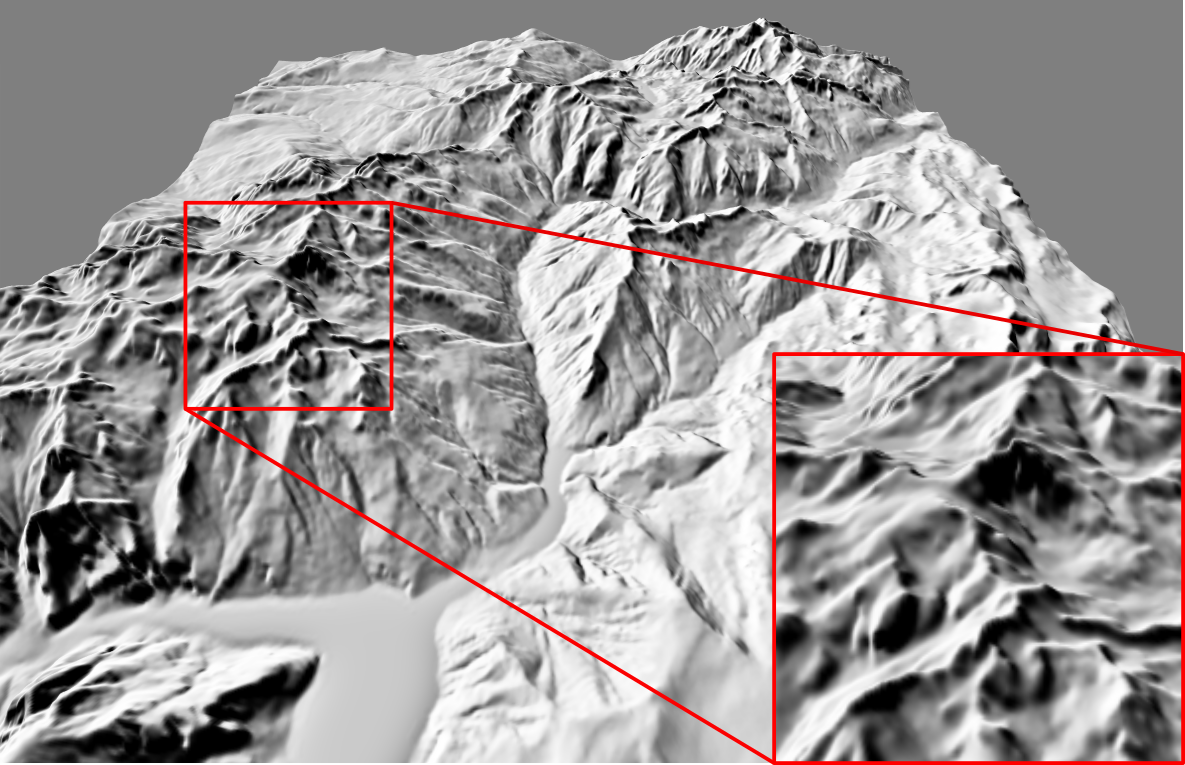
\includegraphics[width=1.0\linewidth]{Solution/ShadeWatercolor.png}
  \caption{Fonction aquarelle de Bousseau et al. \cite{bousseau2006interactive}}
 \end{subfigure}
 \caption{\label{fig:comparaisonFusion} Comparaison entre différente type de fusion.($\alpha =  270\degres$ (Est), $\gamma = 45\degres$ , $\sigma = 30$) Nous observons que les deux fonction \textit{overlay} font plus ressortir l'ombrage, cependant la méthode "aquarelle" évite de perdre certaines aspérités lorsqu'elles sont dans une partie très éclairée ou très sombre.}
\end{figure*}


\section{Les ombres portées}
\subsection{Calcul des ombres portées}
Les ombres portées ne sont pas calculées de la même manière que l'ombrage. Pour ces ombres-là, l'information nécessaire est : quelle est la forme de l’objet qui bloque la lumière. Pour ce faire il existe différentes techniques (shadow maps, shadow volume, etc..), nous renvoyons le lecteur à l'état de l'art \cite{woo1990survey} pour plus d'information. Celle qui nous intéresse est une technique dite de \textit{Ray Marching}. Elle a pour avantage d'être facilement applicable sur une carte de hauteur et permet d'avoir un vecteur de lumière différent par point. 
Le principe est assez simple : en chaque point nous laçons un rayon dans la direction de la lumière et nous vérifions s'il intercepte un objet ou non. Dans notre cas, comme nous partons d'une carte de hauteur, nous avançons pas par pas et nous vérifions si nous sommes en dessous ou non de la hauteur du point courant. Cela permet d'obtenir une carte  où $1$ indique que la lumière passe et $0$ l'inverse (Fig. \ref{fig:raymarching}). 


\begin{figure}
\centering
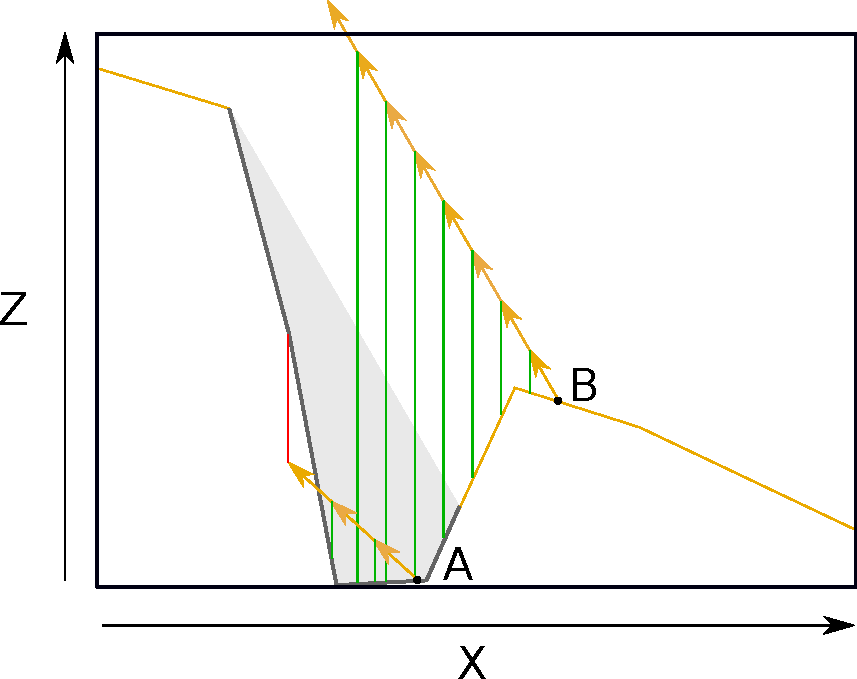
\includegraphics[width=0.5\linewidth]{Solution/raymarching.pdf}
\caption{\label{fig:raymarching} Raymarching sur deux pixel A et B avec en jaune les vecteurs lumières et en vert et rouge la distance par rapport au terrain après chaque pas. A est dans l'ombre, B est dans la lumière}
\end{figure}
\subsection{Abstraction des ombres portées }

Cependant la forme des ombres obtenues n'est pas vraiment conforme au style Novat. Dans les panoramas les ombres portées sont très anguleuses et très marquées or les nôtres se basent sur la forme du terrain qui est plus continue. Parmi les filtres possibles pour transformer la carte des ombres portées, il y a la morphologique mathématique qui est utilisée pour abstraire les formes (utilisée par exemple par Bousseau et al. dans leur rendu aquarelle \cite{bousseau2006interactive}). Cela consiste à traiter un ensemble $A$ à l'aide d'un autre ensemble $B$ appelé élément structurant qui sert de sonde. Pour chaque position de l’élément structurant, nous vérifions s'il est inclus ou non dans l'ensemble initial. À partir de cette information, et d'un opérateur, nous construisons un ensemble de sortie. De notre coté , nous utilisons l’opérateur de fermeture de $A$ par $B$ qui est la succession de l’opérateur de dilatation de $A$ par $B$ suivit de l’opérateur d’érosion du résultat par $B$ :
\begin{equation} 
A \bullet B  = (A \oplus B) \ominus B
\end{equation}
Avec l’opérateur d’érosion : 
\begin{equation} 
A \ominus B  = \{ x \mid \forall a \in A, B_a \cap A = \emptyset   \}
\end{equation}
Et l’opérateur de dilatation : 
\begin{equation} 
A \oplus B  = \{x \mid \forall a \in A, B_a \cap A \neq \emptyset  \}
\end{equation}
Avec x les pixels de l'image et $B_a$ qui correspond à $B$ centré en $a$. 



Dans notre solution $A$ représente l'ensemble des pixels dans l'ombre $(=0)$ et nous utilisons un carré de $5x5$ pixels comme élément structurant (Fig \ref{fig:pyramide_morpho} et \ref{fig:comparaisonMorpho}).
\begin{figure}[h!]
\centering
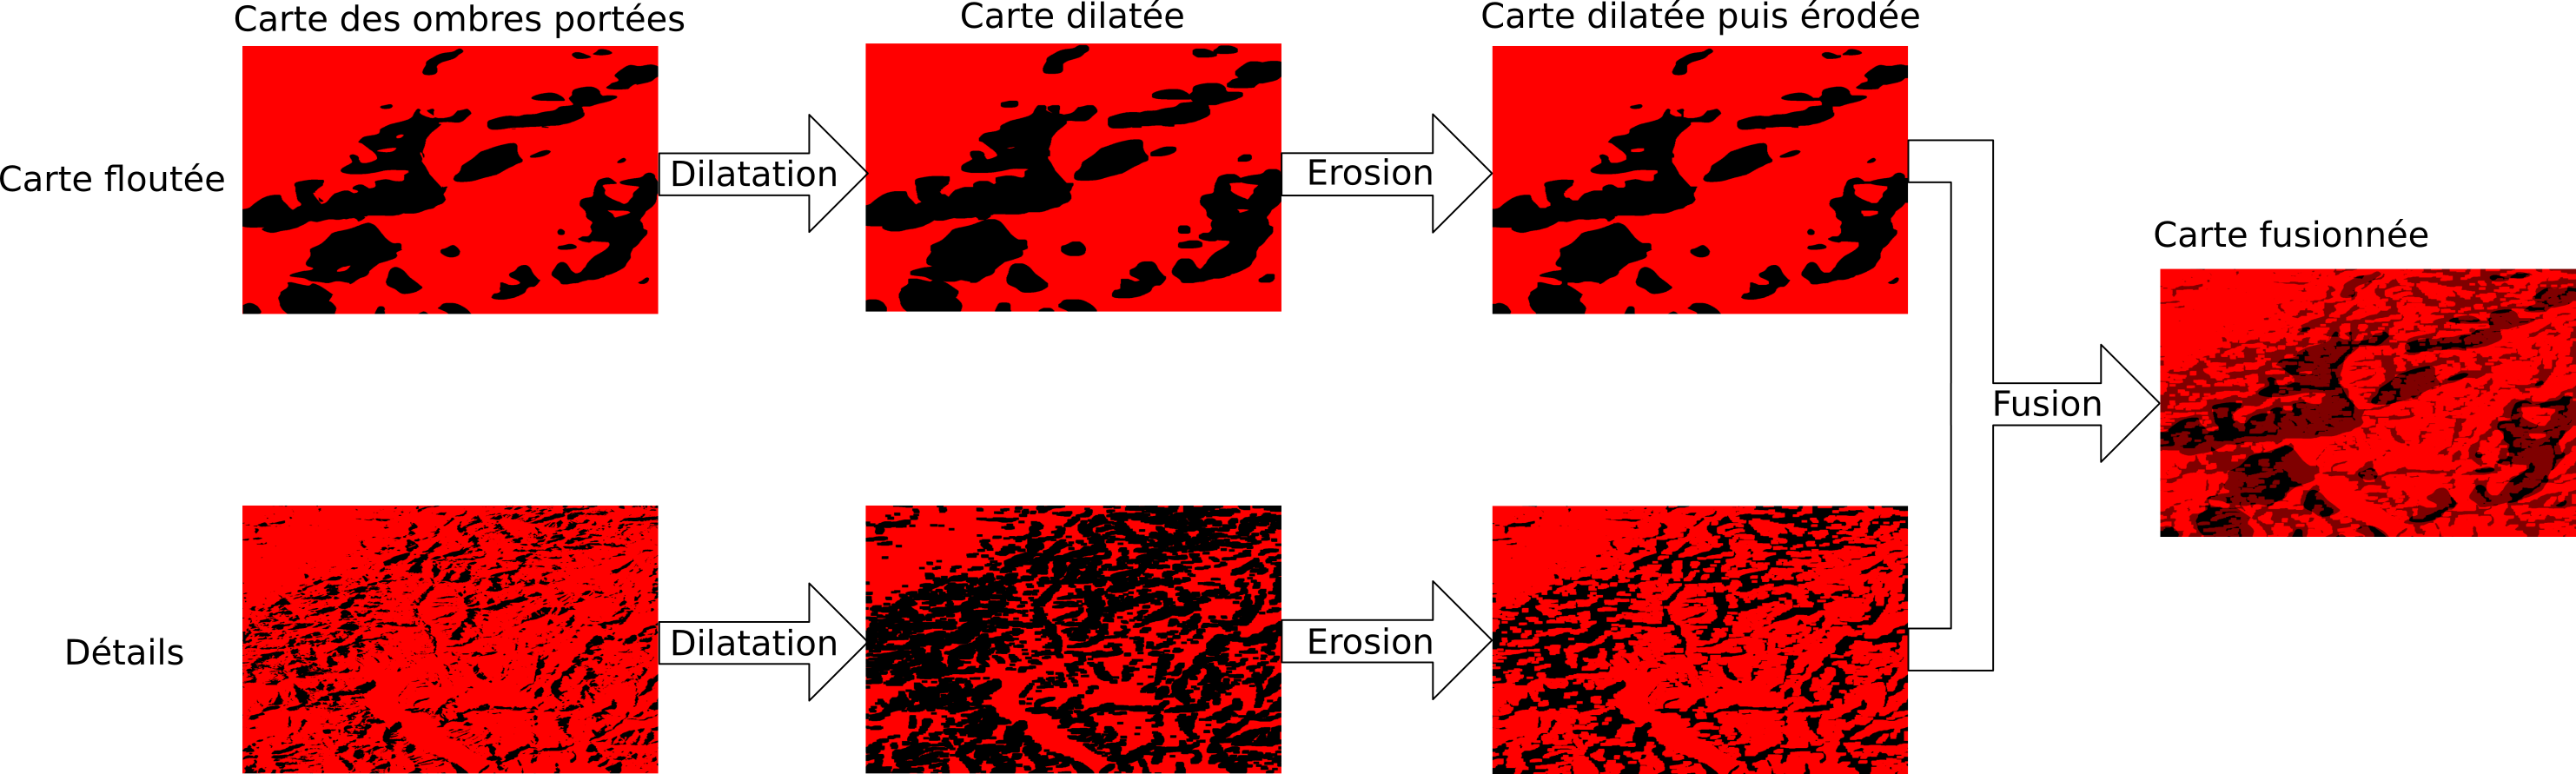
\includegraphics[width=1.0\linewidth]{Solution/pyramide_Laplace_image_morpho.png}

\caption{\label{fig:pyramide_morpho}L'ouverture puis la fusion des ombres portées}
\end{figure}


\begin{figure*}[h!]
\centering
 \begin{subfigure}[t]{0.47\textwidth}
 \centering
 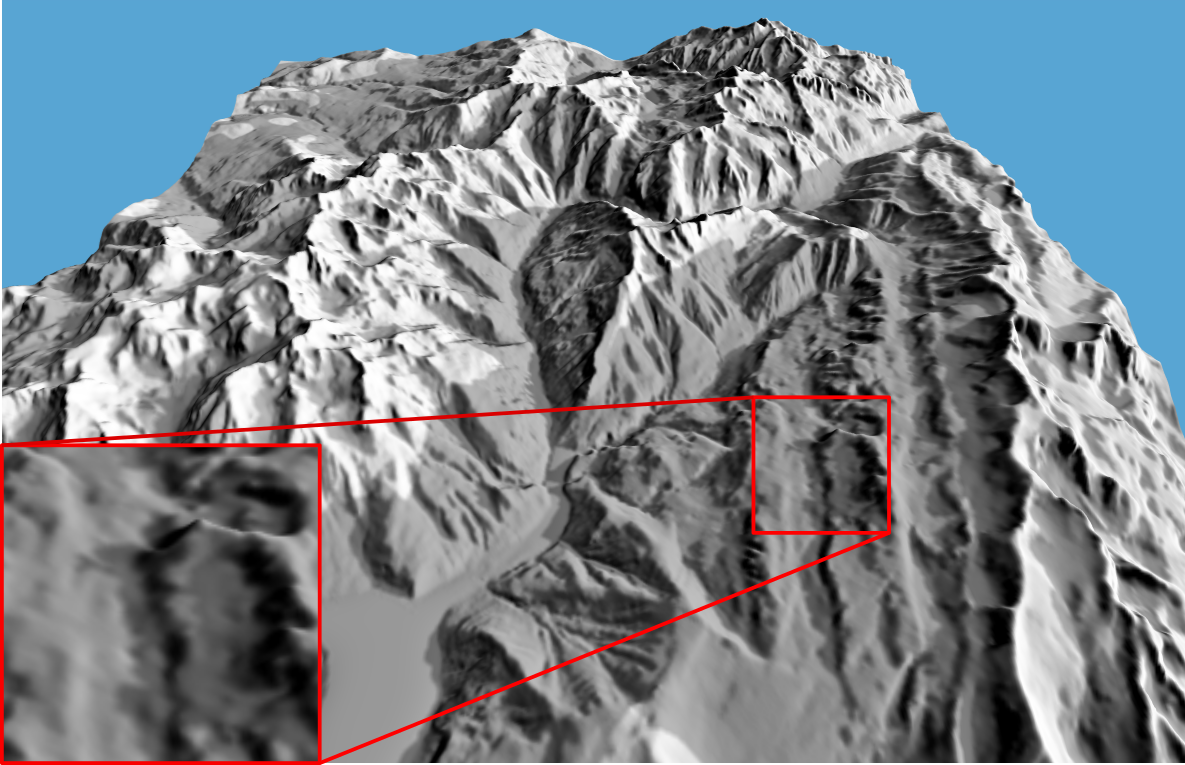
\includegraphics[width=1.0\linewidth]{Solution/sansMorpho.png}
 \caption{Sans abstraction des formes}
 \end{subfigure}
 \begin{subfigure}[t]{0.47\textwidth}
 \centering
 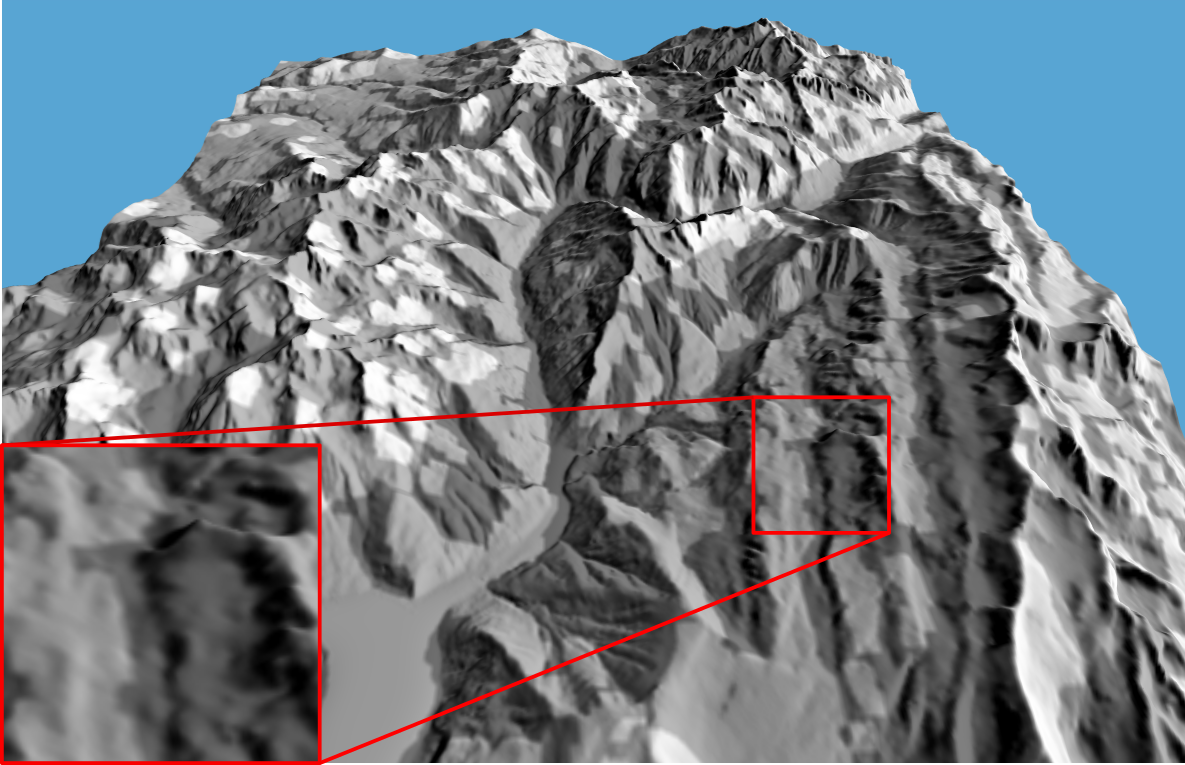
\includegraphics[width=1.0\linewidth]{Solution/avecMorpho.png}
 \caption{Avec abstraction des formes}
 \end{subfigure}
 \caption{\label{fig:comparaisonMorpho} Comparaison avec et sans abstraction des formes avec la morphologie mathématique ($\alpha =  270\degres$ (Est), $\gamma = 10\degres$ , $\sigma = 30$).}
\end{figure*}
\clearpage
\subsection{Multi Échelles et fusion}

Nous utilisons la même méthode pour les ombres portées qu'avec l'ombrage, c'est-à-dire que nous utilisons les deux mêmes échelles pour générer les ombres portées de manière indépendante pour les fusionner ensuite. Cependant la technique de fusion n'est pas la même. En effet, comme les cartes des ombres portées ne sont composées que de 0 et de 1, une simple interpolation linéaire suffit à faire une fusion acceptable. 


Enfin nous fusionnons les ombres portées avec l'ombrage avec l’équation \ref{equationFusionOMOP} qui permet d'ajouter de manière discrète les ombres portées sans masquer la variation de l'ombrage (voir Figure \ref{fig:shadow_shade}). 
\begin{equation}
\label{equationFusionOMOP}
O = OM . \frac{OP+1}{2}
\end{equation} 
Avec $OP$ la valeur des ombres portées au pixel courant, $OM$ la valeur de l'ombrage sur ce même pixel et $O$ l’ombrage final.

\begin{figure}[h!]
\centering
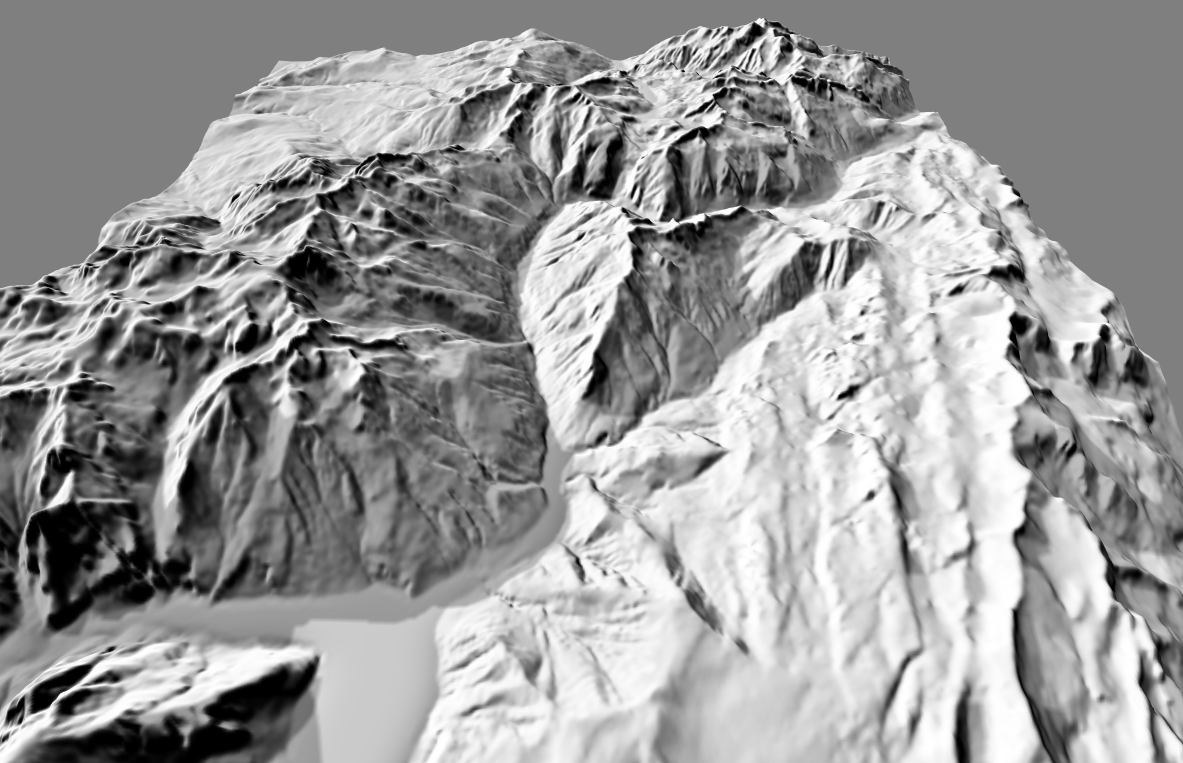
\includegraphics[width=1.0\linewidth]{Solution/shadow_shade.png}
\caption{\label{fig:shadow_shade}Fusion de l'ombrage avec les ombres portées. ($\alpha =  45\degres$ (Nord-Ouest), $\gamma = 20\degres$ , $\sigma = 30$)}
\end{figure}





\chapter{Implémentation et résultats}
\begin{figure*}[h!]

   \centering
   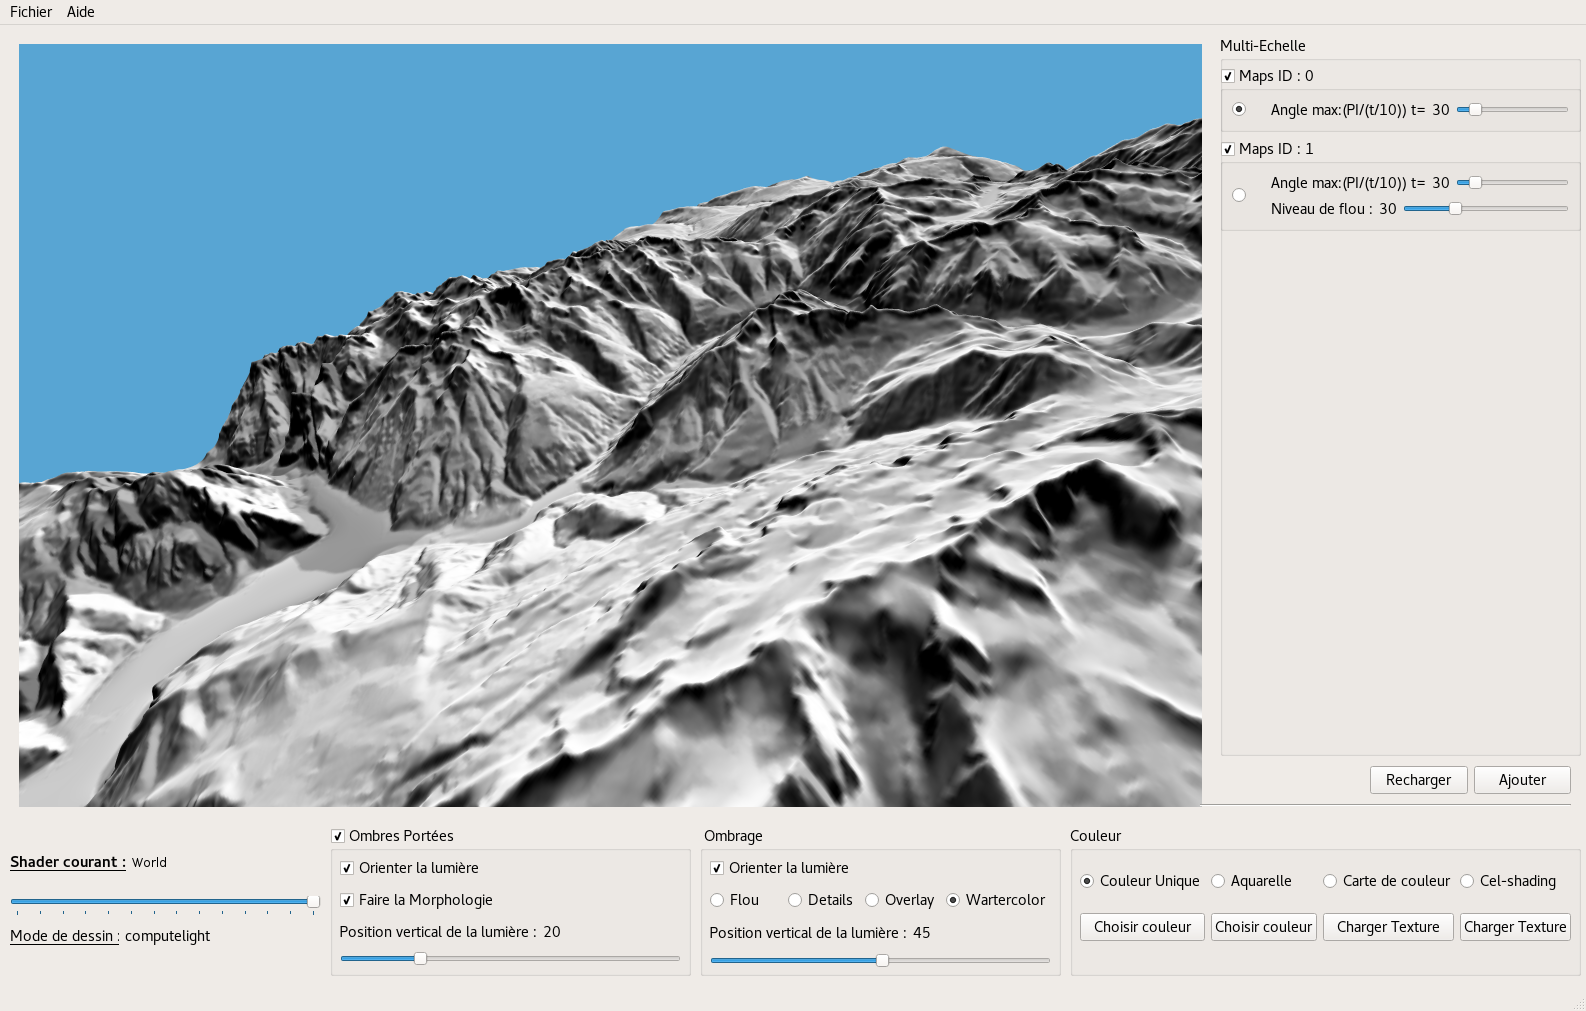
\includegraphics[width=1.0\linewidth]{Resultats/interface.png}
   \caption{Interface de notre prototype}
\end{figure*}

\section{Degrés de libertés}
Dans notre implémentation, nous avons fait le choix de laisser des paramètres que l'utilisateur peut modifier  afin d'être plus proche de ce que pourrait donner un logiciel de rendu de panorama "à la Novat". Dans un premier temps, il peut choisir un ou plusieurs MNT (à condition qu'ils soient continus et que la carte reste rectangulaire). Pour modifier le rendu des ombres, il peut modifier les paramètres de l'ombrage (élévation de la lumière et orientation ou non de la lumière), des ombres portées (élévation de la lumière, orientation ou non de la lumière et abstraction ou non des formes), du multi-echelle (quantité de flou, manière de fusionner les ombrages) et de mise en couleur (unie, aquarelle, carte de couleur ou cel-shading). 
\section{Implémentation}
Notre système de rendu est implémenté en C++ 14 et QT 5.10. Le rendu en lui même est fait en OpenGL et GLSL 4.5 et la plupart des calculs sont faits sur GPU, dans les shaders, avec plusieurs passes successives.  La taille du widget de rendu 3D fait 1200*780 pixels. Notre rendu comprend une camera, une lumière,  ainsi qu'un maillage généré à partir d'un ou plusieurs modèles numériques de terrain (MNT). Pour notre rendu sur la région de l'Alpe d'Huez, nos données font $800*1200$ avec un pas de $25$m et donc couvrent $24$km$^2$, il en résulte un maillage de $5748006$ triangles. Avec une carte graphique \textit{NVIDIA Quadro 6000}, nous avons un rendu à $60$ images par seconde en moyenne sans les ombres portées, $20$ avec, ce qui permet d'avoir un logiciel interactif.  

\paragraph*{Modèle Numérique de Terrain (MNT) : } C'est une carte de hauteur sous la forme d'une dalle carrée de taille variable en fonction de son niveau de détail. Il y a $4$ niveaux de détails proposés par l'IGN : $75$m, $25$m, $5$m et $1$m qui représentent la distance entre chaque donnée. Ainsi une dalle avec un niveau de détail de $25$m fera $4$km$^{2}$, et une dalle avec un niveau de détail de 1m fera $1$km$^{2}$. Les MNT utilisés dans ce projet sont récupérés sur le site de l'Institut national de l'information géographique et forestière (IGN). Ce site permet d'obtenir un ensemble de dalles continues personnalisé.   




\section{Résultats}
Voici un ensemble de résultats que nous avons produits principalement sur le relevé topologique de la région l'Alpes d'Huez (6 dalles avec un niveau de détail de $25$m). $\alpha$ correspond à l'orientation de l'azimut de la lumière globale, $\gamma_o$  l'élévation de la lumière pour l'ombrage, $\gamma_p$ l'élévation de la lumière pour les ombres portées et $\sigma$ la quantité de flou appliqué sur la $2^e$ échelle.  

\begin{figure*}[h!]
\centering
 \begin{subfigure}[t]{0.32\linewidth}
 \centering
 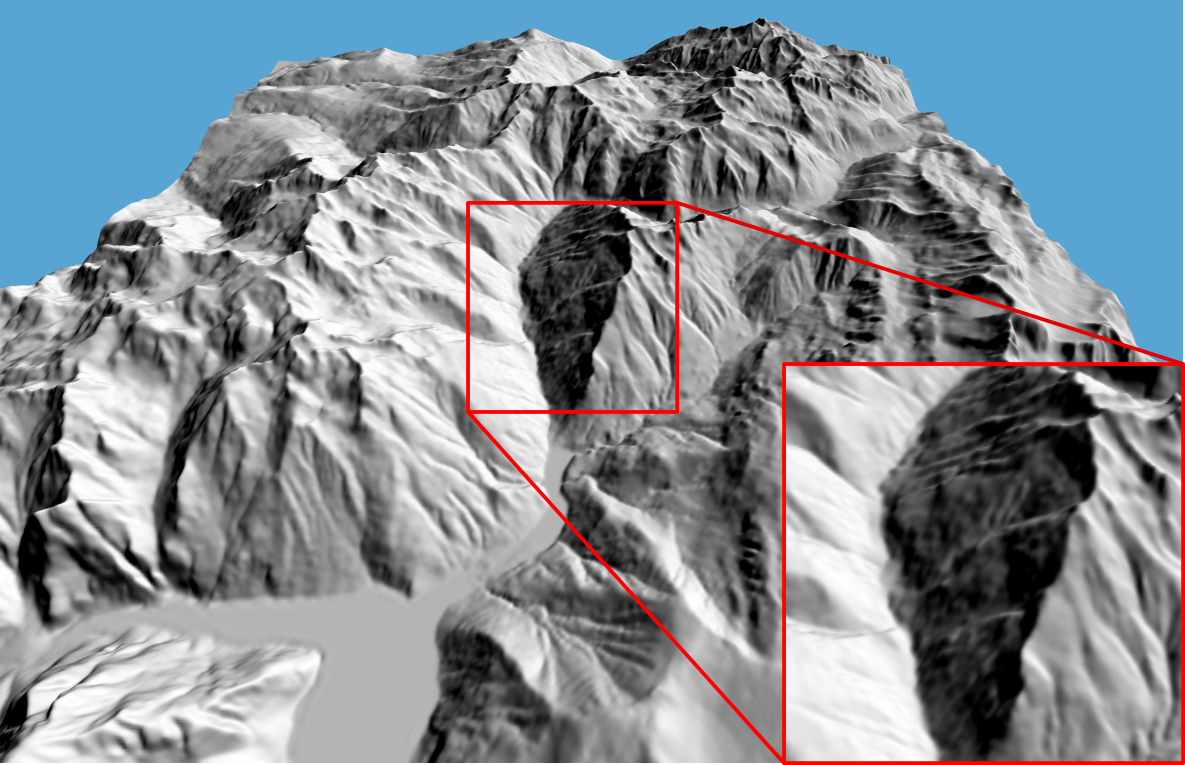
\includegraphics[width=1.0\linewidth]{Resultats/lambertien.png}
 \caption{Lambertien classique }
 \end{subfigure}
 \begin{subfigure}[t]{0.32\linewidth}
 \centering
 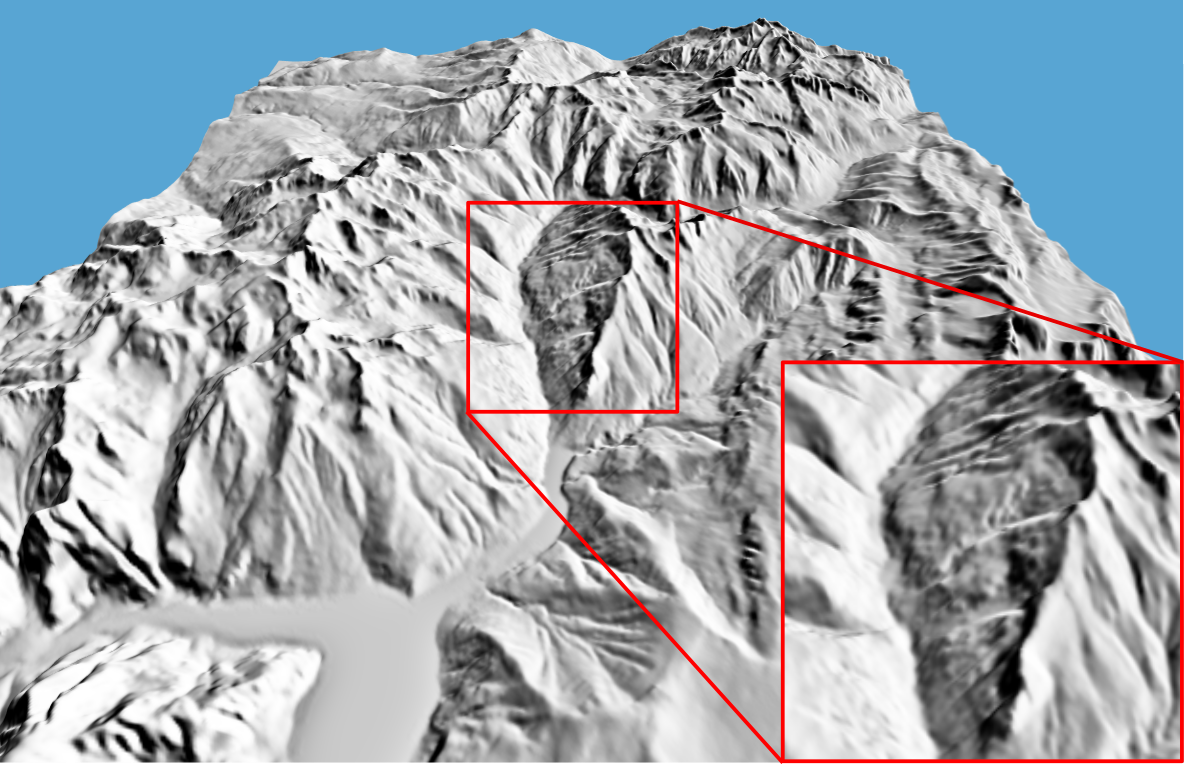
\includegraphics[width=1.0\linewidth]{Resultats/ombrage.png}
  \caption{Notre méthode}
 \end{subfigure}
  \begin{subfigure}[t]{0.32\linewidth}
 \centering
 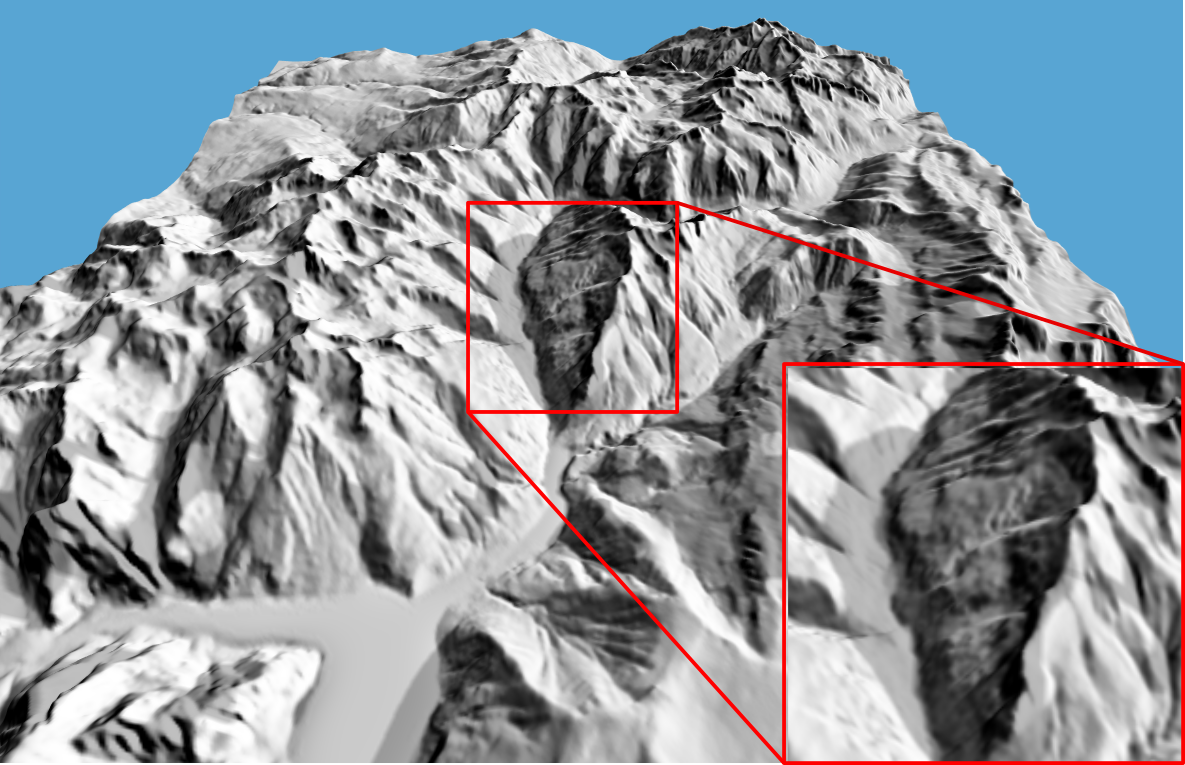
\includegraphics[width=1.0\linewidth]{Resultats/ombre_portee.png}
  \caption{Notre méthode avec les ombres portées}
 \end{subfigure}
 \caption{Comparaison de notre méthode avec un Lambertien classique ($\alpha = 270\degres$ (Est) $\gamma_o = 45\degres$ , $\gamma_p = 20\degres$, $\sigma = 30$).}
\end{figure*}



\begin{figure*}[h!]
\centering
 \begin{subfigure}[t]{0.24\linewidth}
   \centering
   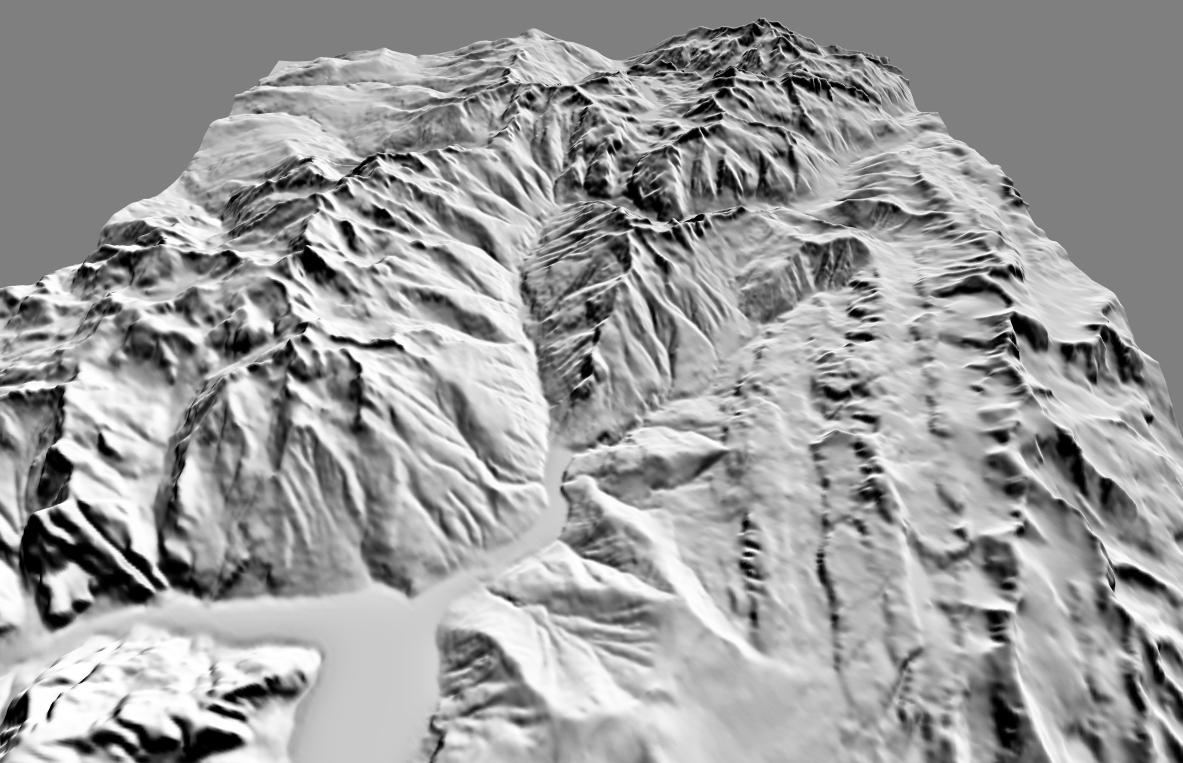
\includegraphics[width=1.0\linewidth]{Resultats/2_nord_our.png}
   \caption{$\alpha = 0\degres$ (Nord)}
 \end{subfigure}
 \begin{subfigure}[t]{0.24\linewidth}
   \centering
   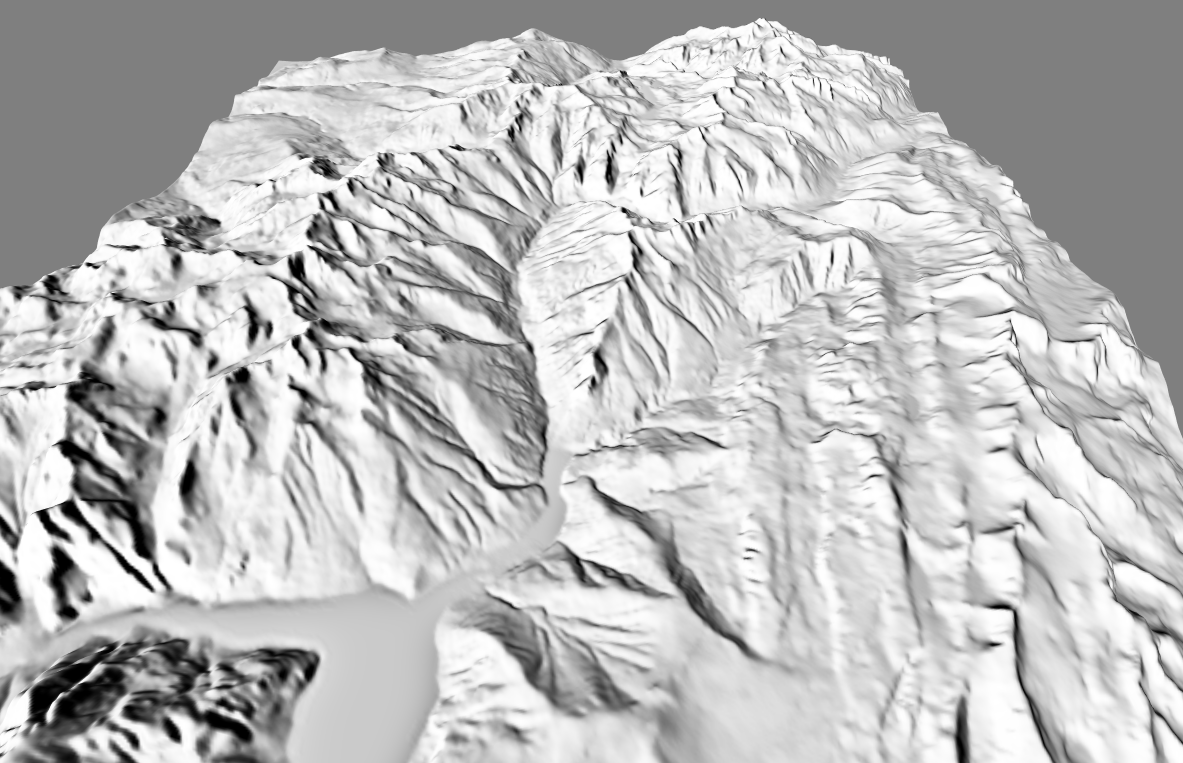
\includegraphics[width=1.0\linewidth]{Resultats/2_sud_our.png}
   \caption{$\alpha = 180\degres$ (Sud)}
 \end{subfigure}
 \begin{subfigure}[t]{0.24\linewidth}
   \centering
   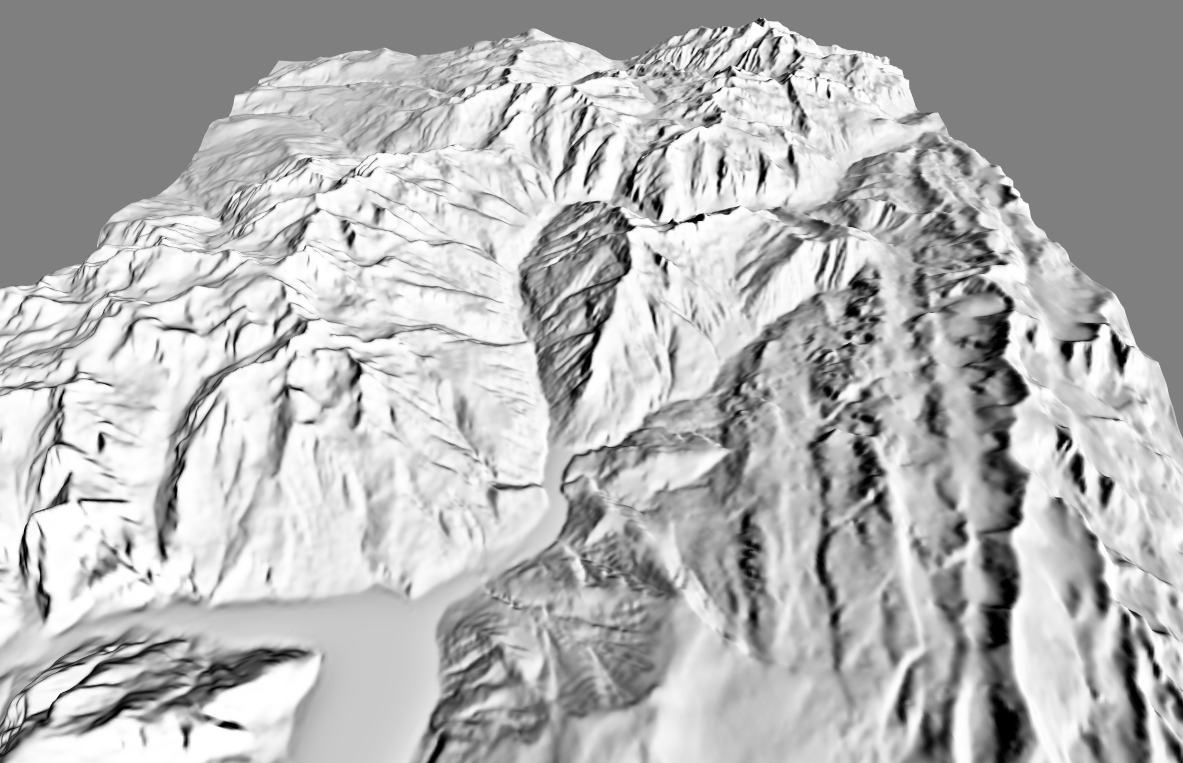
\includegraphics[width=1.0\linewidth]{Resultats/2_est_our.png}
   \caption{$\alpha = 270\degres$ (Est)}
 \end{subfigure}
 \begin{subfigure}[t]{0.24\linewidth}
   \centering
   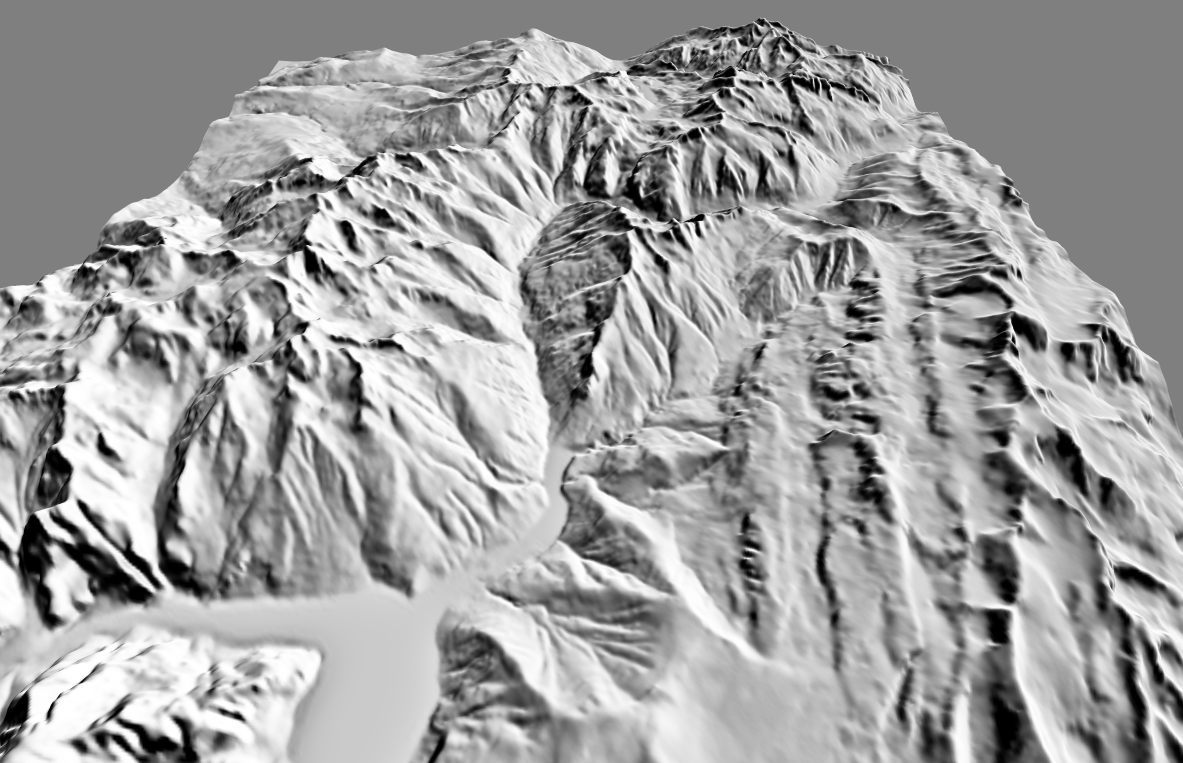
\includegraphics[width=1.0\linewidth]{Resultats/2_nordest_our.png}
   \caption{$\alpha = 315\degres$ (Nord-Est)}
 \end{subfigure}
  \begin{subfigure}[t]{0.24\linewidth}
   \centering
   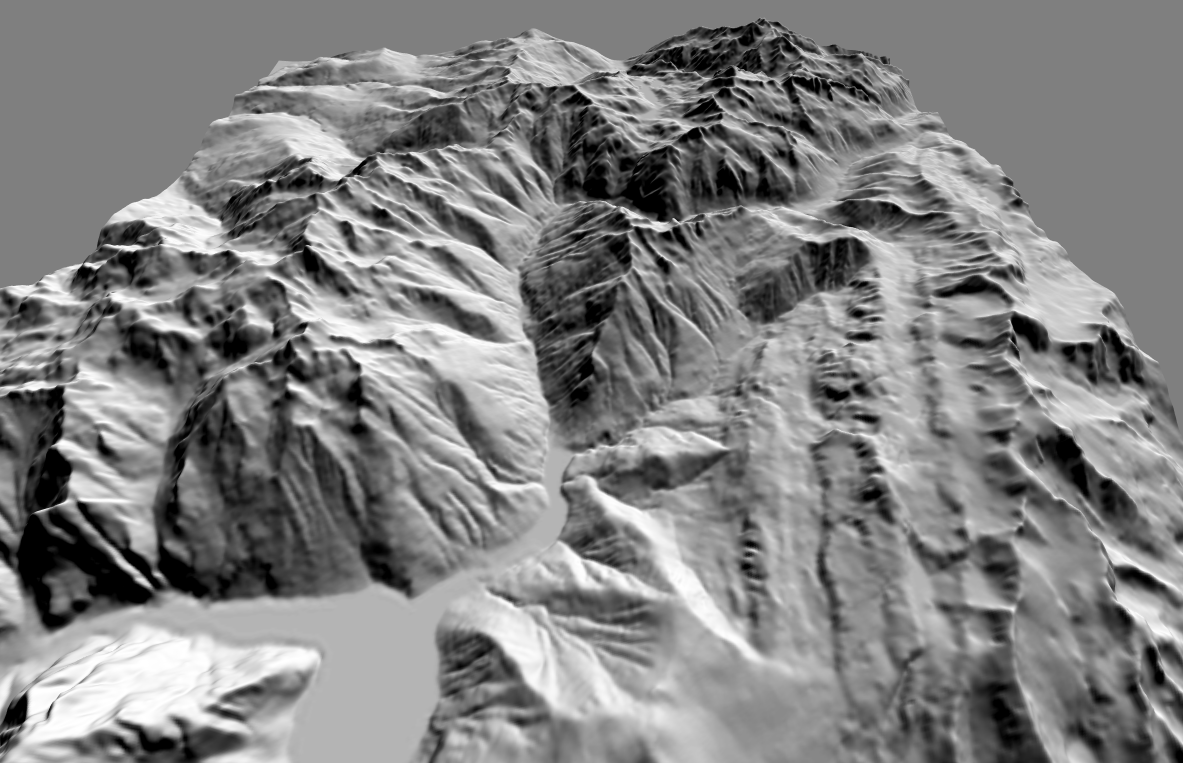
\includegraphics[width=1.0\linewidth]{Resultats/2_nord_lambert.png}
   \caption{$\alpha = 0\degres$ (Nord)}
 \end{subfigure}
 \begin{subfigure}[t]{0.24\linewidth}
   \centering
   \includegraphics[width=1.0\linewidth]{Resultats/2_sud_lambert.png}
   \caption{$\alpha = 180\degres$ (Sud)}
 \end{subfigure}
 \begin{subfigure}[t]{0.24\linewidth}
   \centering
   \includegraphics[width=1.0\linewidth]{Resultats/2_est_lambert.png}
   \caption{$\alpha = 270\degres$ (Est)}
 \end{subfigure}
 \begin{subfigure}[t]{0.24\linewidth}
   \centering
   \includegraphics[width=1.0\linewidth]{Resultats/2_nordest_lambert.png}
   \caption{$\alpha = 315\degres$ (Nord-Est)}
 \end{subfigure}
 \caption{Comparaison entre notre méthode (ligne du haut) et un Lambertien classique (ligne du bas) avec plusieurs orientations du soleil. ( $\gamma_o = 45\degres$ , $\sigma = 30$)}
\end{figure*}


\begin{figure*}[h!]
\centering
 \begin{subfigure}[t]{0.24\linewidth}
   \centering
   \includegraphics[width=1.0\linewidth]{Resultats/3_our_5.png}
   \caption{$\gamma_o = 5\degres$)}
 \end{subfigure}
 \begin{subfigure}[t]{0.24\linewidth}
   \centering
   \includegraphics[width=1.0\linewidth]{Resultats/3_our_20.png}
   \caption{$\gamma_o = 20\degres$}
 \end{subfigure}
 \begin{subfigure}[t]{0.24\linewidth}
   \centering
   \includegraphics[width=1.0\linewidth]{Resultats/3_our_50.png}
   \caption{$\gamma_o = 50\degres$}
 \end{subfigure}
 \begin{subfigure}[t]{0.24\linewidth}
   \centering
   \includegraphics[width=1.0\linewidth]{Resultats/3_our_70.png}
   \caption{$\gamma_o = 70\degres$}
 \end{subfigure}
  \begin{subfigure}[t]{0.24\linewidth}
   \centering
   \includegraphics[width=1.0\linewidth]{Resultats/3_lambert_5.png}
   \caption{$\gamma_o = 5\degres$}
 \end{subfigure}
 \begin{subfigure}[t]{0.24\linewidth}
   \centering
   \includegraphics[width=1.0\linewidth]{Resultats/3_lambert_20.png}
   \caption{$\gamma_o = 20\degres$}
 \end{subfigure}
 \begin{subfigure}[t]{0.24\linewidth}
   \centering
   \includegraphics[width=1.0\linewidth]{Resultats/3_lambert_50.png}
   \caption{$\gamma_o = 50\degres$}
 \end{subfigure}
 \begin{subfigure}[t]{0.24\linewidth}
   \centering
   \includegraphics[width=1.0\linewidth]{Resultats/3_lambert_70.png}
   \caption{$\gamma_o = 70\degres$}
 \end{subfigure}
 \caption{Comparaison entre notre méthode (ligne du haut) et un Lambertien classique (ligne du bas) avec plusieurs élévations du Soleil ( $\alpha = 270\degres$ (Est) , $\sigma = 30$). }
\end{figure*}



\begin{figure*}[h!]
\centering
 \begin{subfigure}[t]{0.24\linewidth}
   \centering
   \includegraphics[width=1.0\linewidth]{Resultats/4_our_5.png}
   \caption{$\sigma = 5$}
 \end{subfigure}
 \begin{subfigure}[t]{0.24\linewidth}
   \centering
   \includegraphics[width=1.0\linewidth]{Resultats/4_our_20.png}
   \caption{$\sigma = 20$}
 \end{subfigure}
 \begin{subfigure}[t]{0.24\linewidth}
   \centering
   \includegraphics[width=1.0\linewidth]{Resultats/4_our_50.png}
   \caption{$\sigma = 50$}
 \end{subfigure}
 \begin{subfigure}[t]{0.24\linewidth}
   \centering
   \includegraphics[width=1.0\linewidth]{Resultats/4_our_100.png}
   \caption{$\sigma = 100$}
 \end{subfigure}
 \caption{Comparaison entre plusieurs niveaux de flou ($\alpha = 315\degres$ (Nord-Est), $\gamma_o = 45\degres$).}
\end{figure*}

\begin{figure*}[h!]
\centering
 \begin{subfigure}[t]{0.49\linewidth}
   \centering
   \includegraphics[width=1.0\linewidth]{Resultats/5_our_nonorien.png}
   \caption{Sans orientation}
 \end{subfigure}
 \begin{subfigure}[t]{0.49\linewidth}
   \centering
   \includegraphics[width=1.0\linewidth]{Resultats/5_our_orien.png}
   \caption{Avec orientation}
 \end{subfigure}
 \caption{Comparaison avec et sans l'orientation de la lumière mais avec le multi-échelle ($\alpha = 315\degres$(Nord-Est), $\gamma_o = 45\degres$ , $\sigma = 30$).}
\end{figure*}

\begin{figure*}[h!]
\centering
 \begin{subfigure}[t]{0.32\linewidth}
 \centering
 \includegraphics[width=1.0\linewidth]{Resultats/aquarelle.png}
 \caption{Aquarelle}
 \end{subfigure}
 \begin{subfigure}[t]{0.32\linewidth}
 \centering
 \includegraphics[width=1.0\linewidth]{Resultats/colorMap.png}
  \caption{\label{fig:degradeColor}Rampe de couleur dégradé}
 \end{subfigure}
  \begin{subfigure}[t]{0.32\linewidth}
 \centering
 \includegraphics[width=1.0\linewidth]{Resultats/cel_shading.png}
  \caption{Cel-shading}
 \end{subfigure}
 \caption{\label{fig:colorOmbre} Comparaison des méthodes de colorisation avec des couleurs données par Arthur Novat($\alpha = 270\degres$ (Est) $\gamma_o = 45\degres$ , $\gamma_p = 20\degres$, $\sigma = 30$). }
\end{figure*}


\begin{figure*}[h!]
\centering
 \begin{subfigure}[t]{0.49\linewidth}
   \centering
   \includegraphics[width=1.0\linewidth]{Resultats/7_high_1.png}
   \caption{$\alpha = 45\degres$ (Nord-Ouest)}
 \end{subfigure}
 \begin{subfigure}[t]{0.49\linewidth}
   \centering
   \includegraphics[width=1.0\linewidth]{Resultats/7_high_2.png}
   \caption{$\alpha = 270\degres$ (Est)}
 \end{subfigure}
 \caption{Terrain avec une résolution de $1$m ($\gamma_o = 45\degres$ , $\gamma_p = 30\degres$, $\sigma = 100$).}
\end{figure*}

\begin{figure*}[h!]

   \centering
   \includegraphics[width=1.0\linewidth]{Resultats/7_grenoble.png}
   \caption{Vallée de Grenoble colorisée avec la même rampe de couleur que la Figure \ref{fig:degradeColor} ($\alpha = 270\degres$ (Est) $\gamma_o = 45\degres$ , $\gamma_p = 20\degres$, $\sigma = 30$).}
\end{figure*}






\chapter{Validation}


\section{Entretien avec Arthur Novat}
Pour valider notre contribution, nous nous sommes dans un premier temps tournés vers Arthur Novat. Comme nous avons essayé de nous rapprocher le plus possible des panoramas de l'atelier Novat, il est l'expert le plus fiable pour juger et critiquer nos résultats. Nous avons donc fait une interview en lui montrant nos résultats pour savoir ce qu'il en pensait. Le retour est positif pour l'ombrage, un peu moins pour les ombres portées. 

Notre principale contribution qui s’attaquait à la lisibilité du terrain est un succès, Arthur Novat nous dit : "Il n'y a plus de zone bouchée et il y a suffisamment de variation dans les zones éclairées". Cela signifie que notre ombrage est suffisamment varié pour qu'il puisse y avoir une bonne lecture du terrain. De plus il rajoute : "C'est à peu près ce que je m'imagine quand je regarde une carte d'état major". Il reste encore des éléments dans l’ombrage à travailler qui sont plus de l'ordre artistique mais notre contribution ne portait pas sur cette question qui viendra dans un second temps.  



Du coté des ombres portées, c'est plus mitigé car notre solution est incomplète pour correspondre au style Novat. Il nous dit : "Les ombres portées ne devraient être que sur les zones importantes". Ensuite, "Plus on va vers un soleil rasant, plus les ombres portées vont être différentes du relief", c'est-à-dire qu'il ne faut pas que les ombre portées débordent trop sur les autres montagnes. C'est un élément auquel nous avons pensé mais qui rentre dans le cadre des travaux futurs.


\section{Comparaison avec un rendu classique}
Notre contribution sur l'ombrage pourrait aussi être validée par la comparaison plus formelle entre un Lambertien et notre méthode. En effet nous avons fait un ombrage de manière à mieux voir les variations dans le terrain. Un bon indicateur pour mesurer les variations dans une image est son gradient. Ainsi nous pouvons comparer les gradients entre la carte de hauteur, un ombrage Lambertien et notre méthode d'ombrage (cf Fig. \ref{fig:comparaisonGradient}). La comparaison que nous avons fait est seulement visuelle. Or une alternative serait d'utiliser des outils statistiques pour par exemple déterminer s'il y a une corrélation local entre les gradients. Néanmoins une telle observation peut donner des éléments de mesure mais risque d'être peu informative sur la perception globale de l'image.
\begin{figure*}[h!]
\centering
 \begin{subfigure}[t]{0.32\linewidth}
 \centering
 \includegraphics[width=1.0\linewidth]{Resultats/gradient_hauteur.png}
 \caption{Carte de hauteur}
 \end{subfigure}
 \begin{subfigure}[t]{0.32\linewidth}
 \centering
 \includegraphics[width=1.0\linewidth]{Resultats/gradient_lambertien.png}
  \caption{Lambertien classique}
 \end{subfigure}
  \begin{subfigure}[t]{0.32\linewidth}
 \centering
 \includegraphics[width=1.0\linewidth]{Resultats/gradient_our.png}
  \caption{Notre méthode d'ombrage}
 \end{subfigure}
 \caption{\label{fig:comparaisonGradient} Comparaison du gradient de la carte de hauteur avec les gradients de l'ombrage d'un Lambertien et de notre méthode ($\alpha = 45\degres$ (Nord-Ouest), $\gamma_o = 45\degres$, $\sigma = 30$). Nous observons que le gradient de notre méthode a des crêtes plus marquées que dans le Lambertien sans pour autant en rajouter par rapport à la carte de hauteur.}
\end{figure*}

\section{Test sur des utilisateurs}

Une dernière validation possible, mais uniquement faisable quand le rendu sera complet, serait de reprendre l’étude faite dans le cadre de MECOMO (\cite{balzarini2016effectiveness}) qui étudiait comment les utilisateurs regardent et comprennent les panoramas de l'atelier Novat et de la reproduire avec des panoramas rendus automatiquement. Nous pourrions alors comparer les résultats de ces deux études et donc vérifier la qualité du rendu. 


\chapter{Discussions des résultats et travaux futurs}



\begin{figure*}[!h]

   \centering
   \includegraphics[width=1.0\linewidth]{novat/AlpeHuez_pistes.png}
   \caption{Plan des pistes de l'alpe d'Huez par Arthur et Pierre Novat.}
\end{figure*}














Notre méthode permet de mettre en valeur toutes les aspérités d'un terrain en faisant un rendu expressif des ombres. Les résultats sont convaincants cependant la méthode est incomplète et il manque une couche "artistique" pour donner un vrai aspect "Novat" à notre rendu. 
\section{L'ombrage expressif}
	L'ombrage est notre principale contribution au rendu de panorama du style de Pierre Novat. Cependant notre méthode n'est pas encore assez générique. En effet, notre méthode se base uniquement sur une pyramide Laplacienne à deux échelles (Fig. \ref{fig:pyramide}), l'une floue, l'autre détaillée (ce qui suffit pour des cartes hauteur avec un pas de 25m mais qui est très insuffisant pour des cartes avec un pas de 1m). Il faudrait pouvoir la généraliser en pouvant faire un nombre arbitraire d’échelles comme dans le papier d'\textit{exagerated shading}  \cite{rusinkiewicz2006exaggerated}. La question sera alors de savoir comment les fusionner et qu'est-ce que ça signifie de faire un ombrage intermédiaire.  En effet notre méthode utilisant une fonction de type "Overlay", qui ne permet pas de s’étendre facilement à $N$ paramètres. La solution naïve serait de fusionner deux par deux les cartes en remontant (ou descendant les échelles) mais cela voudrait dire que la première échelle (ou la dernière) serait la plus importante ce qui ne correspondrait pas forcément à l'effet attendu. Ensuite nous pourrions changer la fonction de fusion. Nous pensons effectivement que notre fonction actuelle est améliorable. Le problème est que le choix de la fonction de fusion n'est pas un choix qui ne sert qu'à optimiser la lecture. C'est un aussi choix qui influence le style du panorama en augmentant ou diminuant le contraste des certaines ombres (par exemple, notre méthode augmente le contraste de l'ombrage de la partie détaillée au détriment de l'ombrage de la partie floutée (Fig. \ref{fig:comparaisonFusion}). Enfin malgré le fait que nous souhaitons faire un rendu style "Novat", une validation plus formelle de notre méthode d'ombrage devrait êtes faite a l'aide des gradients par exemple. 

D'un autre coté, il y a les ombres portées. Notre méthode inclue des ombres portées multi-échelle mais à la lecture des panoramas de Pierre Novat, il possible qu'un calcul d'ombre portée à une seule échelle suffise (sur les montagnes les plus importantes). Ensuite dans notre méthode, il y a trois points à améliorer. Le premier est l'ajustement local du vecteur lumière. Si nous voulons avoir de l'ombre uniquement sur les zones importantes, il faudrait ajuster la hauteur de ce vecteur, par exemple à la pente. Le second est la forme de ces ombres portées. Nous n'avons pas exploité tout ce que pouvait offrir la morphologie mathématique et une idée qui pourrait être testée est de faire un élément structurant avec une forme orientée dans le sens de la lumière plutôt qu'un simple carré et adapté à la résolution de la carte. Enfin le troisième point est la fusion entre ombres portées et ombrage. Dans notre méthode nous fusionnons les ombres portées avec l'ombrage puis nous ajoutons une couche de couleur. Seulement Arthur Novat nous indique que l'ombrage et les ombres portées sont deux couches de couleur qu'il applique l'une sur l'autre. 

Une fois l'ombrage fait nous avons essayé de colorier notre résultat afin d'avoir un rendu plus proche des panoramas du style de Novat. Nous avons essayé plusieurs méthodes : aquarelle, dégradé de couleur, \textit{cel-shading} (Fig \ref{fig:colorOmbre}. Après avoir les avoir montrées à Arthur Novat, il nous a dit que l’aquarelle ressemblait au $1^{er}$ calque qu'il faisait.  De plus il nous a indiqué que la couleur n'était pas que fonction de l'ombrage mais aussi de l'altitude. Ainsi une idée serait d'utiliser un \textit{xToon} \cite{barla2006x} pour avoir une rampe de couleur à deux dimensions, l'une contrôlée par l'ombrage, l'autre par l'altitude. 

Enfin une partie qui sort de notre contribution mais qui est importante pour la suite est l'aspect artistique qu'il est nécessaire d'ajouter pour donner à l'ombrage et aux ombres portées un rendu plus proche du style Novat. En effet  il faudrait augmenter le contraste dans le faible relief et au contraire le baisser dans le haut relief. "Cela sert à donner de la cohérence" nous dit Arthur Novat. De plus il faut modifier la quantité de relief selon la pente : "plus la zone est pentue, plus le relief est dense" tout en empêchant "que ce soit trop vertigineux". De plus les fonds des vallées devraient plus ressortir. Enfin le dessin des ombres devrait être plus complexe. Il faudrait qu'elles soit dégradées avec uniquement le bord de l'ombre qui soit vraiment sombre, et ajouter de l'occlusion ambiante et de l'inter-réflexion entre les montagnes.

\section{Style Novat}
	Une fois la question de l'ombrage résolue, il restera encore beaucoup de travail pour avoir un vrai rendu de panorama style Novat. Dans un premier temps, il faudrait lier notre méthode d'ombrage à la déformation de montagne fait au LIG pour avoir un vrai aperçu de ce que pourrait donner un panorama style Novat fait de manière "automatique".

Ensuite, il faut rajouter les élément décoratifs : rochers, arbres, maisons et routes. Mais chaque élément demande une attention particulière si nous voulions rester fidèle au style. Chaque élément pose deux questions : où le placer et comment le dessiner. Les rochers par exemple peuvent être placés quand la pente devient trop forte et dessinés à l'aide d'une texture procédurale  \cite{perlin2002improving}  ou des textures définies par l'utilisateur \cite{loi2015programmable}. Même constat pour les arbres qui peuvent être dessinés de la même manière mais il faudrait savoir où les placer (en utilisant d'autres carte de l'IGN par exemple) et comment les placer, car ils sont alignés à la pente. De plus ils possèdent une ombre non négligeable qu'il faudrait prendre en compte dans notre méthode d'illumination. Ensuite pour les maisons c'est encore une autre question car elles représentent assez fidèlement les villages, il faut donc arriver à extraire leur forme de cartes ou de photos pour pouvoir les traduire dans un style Novat. De plus comme pour les sapins, il faut les intégrer à notre modèle d'illumination. Enfin les routes sont peut être un peu plus simples à faire, il faut juste leur donner un aspect continu et "creuser" la montagne là ou elles passent pour les faire ressortir. 

Enfin la dernière chose à faire est d'intégrer des niveaux de détails, c'est-à-dire faire en sorte que plus nous nous éloignons du point de vue, plus les détails s'effacent et plus nous avons un aspect générique. 


\section{Conclusion}
Dans ce rapport nous avons produit deux contributions : l'étude du style de Pierre Novat et le calcul d'un ombrage expressif. Notre rendu répond à la question de comment faire ressortir toutes les variations d'un terrain mais il reste incomplet dans le cadre d'un rendu de style Novat. La principale difficulté dans l'imitation d’œuvres artistiques est qu'il est difficile d'avoir un résultat convainquant dès le premier essai. Dans notre cas nous avons la chance, contrairement aux autres publication dans le même style \cite{bratkova2009artistic}\cite{brown2017real}, d'être en contact direct avec l'artiste et c'est grâce aux discussions avec Arthur Novat que nous avons pu avancer. Mais il est difficile pour lui d'exprimer d'un seul coup tous les algorithmes mentaux qui lui servent à créer ses œuvres. Ainsi il a besoin d'une première solution pour pouvoir dire ce qui manque et de plus en plus préciser ce qui se passe quand il produit ses œuvres. C'est parce que la solution proposée donne une bonne base de relief que nous avons pu collecter des éléments d'information qui permettront d'aller plus loin. Ainsi, ce sont ces échanges continuels qui permettront,  je l'espère, à terme de créer un rendu très proche des panoramas Pierre Novat. 

    
\appendix \chapter{Appendix} 

\section{Quelques paroramas de l'Atelier Novat}


\begin{figure*}[h!]

   \centering
   \includegraphics[width=1.0\linewidth]{novat/Val_Isere.jpg}
   \caption{Val d'Isere, Tignes, 1967 - Pierre Novat.}
\end{figure*}

\begin{figure*}[h!]

   \centering
   \includegraphics[width=1.0\linewidth]{novat/praloup.jpg}
   \caption{Praloup - Arthur et Pierre Novat.}
\end{figure*}

\begin{figure*}[h!]

   \centering
   \includegraphics[width=1.0\linewidth]{novat/3Vallees.jpg}
   \caption{Les 3 Vallées (Val Thorens, Les Menuires, St Martin De Belleville, Meribel, Brides-les-bains, La Tania, Courchevel) , 2007 - Frédérique et Pierre Novat.}
\end{figure*}

\begin{figure*}[h!]

   \centering
   \includegraphics[width=1.0\linewidth]{novat/chamrousse.jpg}
   \caption{Chamrousse, 2005 - Pierre Novat.}
\end{figure*}

\begin{figure*}[h!]

   \centering
   \includegraphics[width=1.0\linewidth]{novat/annecy-ete.jpg}
   \caption{Lac d'annecy en été - Pierre Novat.}
\end{figure*}






%=========================================================


%=========================================================
\backmatter

\bibliographystyle{plain-fr} % plain-fr si rapport en français 
\bibliography{bibfile.bib}

%\cleardoublepage % Goes to an odd page
%\pagestyle{empty} % no page number
%~\newpage % goes to a new even page

\end{document}